% Options for packages loaded elsewhere
\PassOptionsToPackage{unicode}{hyperref}
\PassOptionsToPackage{hyphens}{url}
%
\documentclass[
]{article}
\usepackage{lmodern}
\usepackage{amssymb,amsmath}
\usepackage{ifxetex,ifluatex}
\ifnum 0\ifxetex 1\fi\ifluatex 1\fi=0 % if pdftex
  \usepackage[T1]{fontenc}
  \usepackage[utf8]{inputenc}
  \usepackage{textcomp} % provide euro and other symbols
\else % if luatex or xetex
  \usepackage{unicode-math}
  \defaultfontfeatures{Scale=MatchLowercase}
  \defaultfontfeatures[\rmfamily]{Ligatures=TeX,Scale=1}
\fi
% Use upquote if available, for straight quotes in verbatim environments
\IfFileExists{upquote.sty}{\usepackage{upquote}}{}
\IfFileExists{microtype.sty}{% use microtype if available
  \usepackage[]{microtype}
  \UseMicrotypeSet[protrusion]{basicmath} % disable protrusion for tt fonts
}{}
\makeatletter
\@ifundefined{KOMAClassName}{% if non-KOMA class
  \IfFileExists{parskip.sty}{%
    \usepackage{parskip}
  }{% else
    \setlength{\parindent}{0pt}
    \setlength{\parskip}{6pt plus 2pt minus 1pt}}
}{% if KOMA class
  \KOMAoptions{parskip=half}}
\makeatother
\usepackage{xcolor}
\IfFileExists{xurl.sty}{\usepackage{xurl}}{} % add URL line breaks if available
\IfFileExists{bookmark.sty}{\usepackage{bookmark}}{\usepackage{hyperref}}
\hypersetup{
  pdftitle={epi curious},
  pdfauthor={Ania Kawiecki},
  hidelinks,
  pdfcreator={LaTeX via pandoc}}
\urlstyle{same} % disable monospaced font for URLs
\usepackage[margin=1in]{geometry}
\usepackage{color}
\usepackage{fancyvrb}
\newcommand{\VerbBar}{|}
\newcommand{\VERB}{\Verb[commandchars=\\\{\}]}
\DefineVerbatimEnvironment{Highlighting}{Verbatim}{commandchars=\\\{\}}
% Add ',fontsize=\small' for more characters per line
\usepackage{framed}
\definecolor{shadecolor}{RGB}{248,248,248}
\newenvironment{Shaded}{\begin{snugshade}}{\end{snugshade}}
\newcommand{\AlertTok}[1]{\textcolor[rgb]{0.94,0.16,0.16}{#1}}
\newcommand{\AnnotationTok}[1]{\textcolor[rgb]{0.56,0.35,0.01}{\textbf{\textit{#1}}}}
\newcommand{\AttributeTok}[1]{\textcolor[rgb]{0.77,0.63,0.00}{#1}}
\newcommand{\BaseNTok}[1]{\textcolor[rgb]{0.00,0.00,0.81}{#1}}
\newcommand{\BuiltInTok}[1]{#1}
\newcommand{\CharTok}[1]{\textcolor[rgb]{0.31,0.60,0.02}{#1}}
\newcommand{\CommentTok}[1]{\textcolor[rgb]{0.56,0.35,0.01}{\textit{#1}}}
\newcommand{\CommentVarTok}[1]{\textcolor[rgb]{0.56,0.35,0.01}{\textbf{\textit{#1}}}}
\newcommand{\ConstantTok}[1]{\textcolor[rgb]{0.00,0.00,0.00}{#1}}
\newcommand{\ControlFlowTok}[1]{\textcolor[rgb]{0.13,0.29,0.53}{\textbf{#1}}}
\newcommand{\DataTypeTok}[1]{\textcolor[rgb]{0.13,0.29,0.53}{#1}}
\newcommand{\DecValTok}[1]{\textcolor[rgb]{0.00,0.00,0.81}{#1}}
\newcommand{\DocumentationTok}[1]{\textcolor[rgb]{0.56,0.35,0.01}{\textbf{\textit{#1}}}}
\newcommand{\ErrorTok}[1]{\textcolor[rgb]{0.64,0.00,0.00}{\textbf{#1}}}
\newcommand{\ExtensionTok}[1]{#1}
\newcommand{\FloatTok}[1]{\textcolor[rgb]{0.00,0.00,0.81}{#1}}
\newcommand{\FunctionTok}[1]{\textcolor[rgb]{0.00,0.00,0.00}{#1}}
\newcommand{\ImportTok}[1]{#1}
\newcommand{\InformationTok}[1]{\textcolor[rgb]{0.56,0.35,0.01}{\textbf{\textit{#1}}}}
\newcommand{\KeywordTok}[1]{\textcolor[rgb]{0.13,0.29,0.53}{\textbf{#1}}}
\newcommand{\NormalTok}[1]{#1}
\newcommand{\OperatorTok}[1]{\textcolor[rgb]{0.81,0.36,0.00}{\textbf{#1}}}
\newcommand{\OtherTok}[1]{\textcolor[rgb]{0.56,0.35,0.01}{#1}}
\newcommand{\PreprocessorTok}[1]{\textcolor[rgb]{0.56,0.35,0.01}{\textit{#1}}}
\newcommand{\RegionMarkerTok}[1]{#1}
\newcommand{\SpecialCharTok}[1]{\textcolor[rgb]{0.00,0.00,0.00}{#1}}
\newcommand{\SpecialStringTok}[1]{\textcolor[rgb]{0.31,0.60,0.02}{#1}}
\newcommand{\StringTok}[1]{\textcolor[rgb]{0.31,0.60,0.02}{#1}}
\newcommand{\VariableTok}[1]{\textcolor[rgb]{0.00,0.00,0.00}{#1}}
\newcommand{\VerbatimStringTok}[1]{\textcolor[rgb]{0.31,0.60,0.02}{#1}}
\newcommand{\WarningTok}[1]{\textcolor[rgb]{0.56,0.35,0.01}{\textbf{\textit{#1}}}}
\usepackage{longtable,booktabs}
% Correct order of tables after \paragraph or \subparagraph
\usepackage{etoolbox}
\makeatletter
\patchcmd\longtable{\par}{\if@noskipsec\mbox{}\fi\par}{}{}
\makeatother
% Allow footnotes in longtable head/foot
\IfFileExists{footnotehyper.sty}{\usepackage{footnotehyper}}{\usepackage{footnote}}
\makesavenoteenv{longtable}
\usepackage{graphicx,grffile}
\makeatletter
\def\maxwidth{\ifdim\Gin@nat@width>\linewidth\linewidth\else\Gin@nat@width\fi}
\def\maxheight{\ifdim\Gin@nat@height>\textheight\textheight\else\Gin@nat@height\fi}
\makeatother
% Scale images if necessary, so that they will not overflow the page
% margins by default, and it is still possible to overwrite the defaults
% using explicit options in \includegraphics[width, height, ...]{}
\setkeys{Gin}{width=\maxwidth,height=\maxheight,keepaspectratio}
% Set default figure placement to htbp
\makeatletter
\def\fps@figure{htbp}
\makeatother
\usepackage[normalem]{ulem}
% Avoid problems with \sout in headers with hyperref
\pdfstringdefDisableCommands{\renewcommand{\sout}{}}
\setlength{\emergencystretch}{3em} % prevent overfull lines
\providecommand{\tightlist}{%
  \setlength{\itemsep}{0pt}\setlength{\parskip}{0pt}}
\setcounter{secnumdepth}{-\maxdimen} % remove section numbering

\title{epi curious}
\author{Ania Kawiecki}
\date{9/29/2020}

\begin{document}
\maketitle

{
\setcounter{tocdepth}{2}
\tableofcontents
}
\begin{Shaded}
\begin{Highlighting}[]
\KeywordTok{library}\NormalTok{(tidyverse)}
\KeywordTok{library}\NormalTok{(rethinking)}
\KeywordTok{library}\NormalTok{(dagitty)}
\KeywordTok{library}\NormalTok{(knitr)}
\KeywordTok{library}\NormalTok{(}\StringTok{"ggdag"}\NormalTok{)}
\KeywordTok{library}\NormalTok{(}\StringTok{"ggrepel"}\NormalTok{)}

\KeywordTok{library}\NormalTok{(INLA)}
\KeywordTok{library}\NormalTok{(knitr)}
\KeywordTok{library}\NormalTok{(stringr)}
\KeywordTok{library}\NormalTok{(}\StringTok{"patchwork"}\NormalTok{)}
\KeywordTok{library}\NormalTok{(}\StringTok{"ghibli"}\NormalTok{)}
\KeywordTok{library}\NormalTok{(}\StringTok{"fpp2"}\NormalTok{)}
\end{Highlighting}
\end{Shaded}

\hypertarget{resources}{%
\section{Resources}\label{resources}}

\begin{itemize}
\tightlist
\item
  Intro to Epidemiology
\end{itemize}

Epidemiology,5th edition, Leon Gordis

\begin{itemize}
\tightlist
\item
  Causal inference
\end{itemize}

\href{https://www.hsph.harvard.edu/miguel-hernan/causal-inference-book/}{Causal
Inference: What If, by Miguel A. Hernán, James M. Robins}

\href{http://xcelab.net/rm/statistical-rethinking/}{Statistical
Rethinking: A Bayesian Course with Examples in R and Stan. Second
edition, by Richard McElreath}

\href{https://academic.oup.com/aje/article/155/2/176/108106}{Causal
Knowledge as a Prerequisite for Confounding Evaluation: An Application
to Birth Defects Epidemiology, Hernàn 2002}

\href{https://projecteuclid.org/euclid.ssu/1255440554http://projecteuclid.org/euclid.ssu/1255440554}{Causal
inference in statistics: an overview, Pearl 2009}

\href{https://www.ncbi.nlm.nih.gov/pmc/articles/PMC2836213/}{An
introduction to causal inference, Pearl 2010}

\begin{itemize}
\tightlist
\item
  Models
\end{itemize}

Gelman and Hill 2005

\begin{itemize}
\tightlist
\item
  Forecasts
\end{itemize}

\url{https://otexts.com/fpp2/}

\url{https://medium.com/analytics-vidhya/basics-of-forecast-accuracy-db704b0b001b\#}:\textasciitilde:text=A\%20simple\%20measure\%20of\%20forecast,known\%20as\%20Mean\%20Forecast\%20Error.\&text=The\%20MFE\%20for\%20this\%20forecasting,more\%20than\%20the\%20forecast\%20values.

\begin{itemize}
\tightlist
\item
  ggdag
\end{itemize}

\url{https://ggdag.malco.io/}

\url{https://malco.io/2019/09/17/tidy-causal-dags-with-ggdag-0-2-0/}

\url{https://cran.r-project.org/web/packages/ggdag/vignettes/intro-to-ggdag.html}

\url{https://cran.r-project.org/web/packages/ggdag/vignettes/bias-structures.html}

\begin{itemize}
\tightlist
\item
  spatial
\end{itemize}

satscan user guide

epidemiology 223 notes

\hypertarget{epidemiological-concepts}{%
\section{\texorpdfstring{\textbf{EPIDEMIOLOGICAL
CONCEPTS}}{EPIDEMIOLOGICAL CONCEPTS}}\label{epidemiological-concepts}}

\hypertarget{measures-of-disease-frequency}{%
\subsection{MEASURES OF DISEASE
FREQUENCY}\label{measures-of-disease-frequency}}

\hypertarget{morbidity}{%
\subsubsection{MORBIDITY}\label{morbidity}}

\hypertarget{prevalence}{%
\subsubsection{prevalence}\label{prevalence}}

Proportion of the population affected at time t = snapshot of disease.

Units: 0-1 or 0-100\%

\[\frac{cases\:at\:time\:t\:(new + existing)}{total\:population\:at\:time\:t}\]
Risk of \emph{being} a case.

\[prevalence = incidence * duration\] It's a bad measure of risk because
it depends on the duration of disease. Chronic diseases will have high
prevalnce, and very fatal diseases will have low prevalence, regardless
of the incidence.

\begin{itemize}
\tightlist
\item
  \textbf{point prevalence}: prevalence at a given timepoint t
\end{itemize}

\[\frac{cases\:at\:time\:t\:(new + existing)}{total\:population\:at\:time\:t}\]

\begin{itemize}
\tightlist
\item
  \textbf{period prevalence}: prevalence at any given timepoint during a
  time period t
\end{itemize}

\[\frac{cases\:observed\:over\:period\:t\:(new + existing)}{total\:population\:at\:midpoint\:of\:period\:t}\]

\hypertarget{incidence}{%
\subsubsection{incidence}\label{incidence}}

Proportion of the population at risk of being affected that does become
affected during a time period t. cases/population * time at risk

\[\frac{new\:cases\:observed\:over\:period\:t}{total\:population\:at\:risk\:during\:period\:t}\]

Risk of \emph{becoming} a case.

\[\frac{cases}{population*time\:at\:risk}\] It measures risk because it
measures events or transitions from affected to not affected state.

\begin{itemize}
\tightlist
\item
  \textbf{cumulative incidence}
\end{itemize}

The population at risk is a crude measure of the population at risk at
the beginning of the time period. It assumes a static population at
risk.

Units: 0-1 or 0-100\% per time interval.

\[\frac{new\:cases\:observed\:over\:period\:t}{total\:population\:at\:risk\:at\:start\:of\:time\:period\:t}\]
Measures average risk. Is apt for short time-periods or static
populations.

\begin{itemize}
\tightlist
\item
  \textbf{incidence density rate}
\end{itemize}

The population at risk is the sum of all the disease-free/ at risk time
periods for each individual. It assumes the risk of each person in the
population does not change over time.

Units: 0- \(\infty\) cases/population-time

\[\frac{new\:cases\:observed\:over\:period\:t}{total\:population-time}\]
Measures risk by taking into account the time elapsed before disease
occured for each individual, thus it also measures the speed at which
disease occurs at a certain timepoint. Is apt for prolonged time-periods
or dynamic populations.

To calculate population-time:

\begin{itemize}
\tightlist
\item
  sum all the disease-free time for each individual.
\item
  estimate:

  \begin{itemize}
  \tightlist
  \item
    count the population-time midway through the time period
  \item
    average the population-time at the beginning and the end of the
    period.
  \end{itemize}
\end{itemize}

\hypertarget{attack-rate}{%
\subsubsection{attack rate}\label{attack-rate}}

Proportion of the exposed individuals that becomes affected during a
time period t.

\[\frac{cases}{exposed}\]

\begin{figure}
\centering
\includegraphics{/Users/annakawiecki/Documents/epi/workshops/akawiecki_pubs/pubs/DAG/notes screenshots/Screen Shot 2020-12-02 at 13.35.40.png}
\caption{Relationship between incidence and prevalence. Gordis}
\end{figure}

\hypertarget{mortality}{%
\subsubsection{MORTALITY}\label{mortality}}

\hypertarget{mortality-rate}{%
\subsubsection{mortality rate}\label{mortality-rate}}

Speed of death in time t.

Measures risk: good measure when disease is mild, bad measure when
disease is very deadly and the case-fatality is high.

\[\frac{deaths\:over\:period\:t}{total\:population\:at\:risk\:during\:time\:period\:t}\]

\begin{itemize}
\tightlist
\item
  \textbf{crude mortality rate}
\end{itemize}

overall deaths

\[\frac{deaths\:over\:period\:t}{total\:population\:at\:risk\:during\:time\:period\:t}\]

\begin{itemize}
\tightlist
\item
  \textbf{specific mortality rate}
\end{itemize}

deaths in a specific subgroup (age, sex, diseased with a certain
disease)

\[\frac{deaths\:in\:subgroup\:over\:period\:t}{population\:at\:risk\:in\:subgroup\:during\:time\:period\:t}\]

\hypertarget{case-fatality-rate}{%
\subsubsection{case fatality rate}\label{case-fatality-rate}}

Proportion of the individuals that become affected by disease X who die
during a time period t.

Measures disease severity

\[\frac{deaths}{cases}\]

\hypertarget{proportionate-mortality}{%
\subsubsection{proportionate mortality}\label{proportionate-mortality}}

Fraction of all the deaths caused by disease X

\[\frac{deaths\:from\:disease\:X}{all\:deaths}\]

\hypertarget{rates}{%
\subsubsection{RATES}\label{rates}}

\hypertarget{crude}{%
\subsubsection{crude}\label{crude}}

overall population

\hypertarget{adjusted}{%
\subsubsection{adjusted}\label{adjusted}}

adjusted rates controlling for confounding factors to remove the effect
of that factor

\begin{itemize}
\tightlist
\item
  \textbf{direct}
\end{itemize}

Apply the specific subgroup rates of each population to a standard
population and calculate the rate on the standard population.

\begin{figure}
\centering
\includegraphics{/Users/annakawiecki/Documents/epi/workshops/akawiecki_pubs/pubs/DAG/notes screenshots/Screen Shot 2020-12-02 at 13.04.03.png}
\caption{direct adjusted example from Gordis}
\end{figure}

\begin{itemize}
\tightlist
\item
  \textbf{indirect}
\end{itemize}

Compare populations: subgroup vs general

SMR = Strandard Mortality Ratio \[SMR= \frac{Observed}{Expected}\]

Expected: Apply the general population rates to each specific subgroup
and add all the cases Observed: add all the observed cases in each
specific subgroup

\begin{figure}
\centering
\includegraphics{/Users/annakawiecki/Documents/epi/workshops/akawiecki_pubs/pubs/DAG/notes screenshots/Screen Shot 2020-12-02 at 13.08.05.png}
\caption{indirect adjusted example from Gordis}
\end{figure}

\hypertarget{diagnostic-test-evaluation-and-screening-tests}{%
\subsection{DIAGNOSTIC TEST EVALUATION AND SCREENING
TESTS}\label{diagnostic-test-evaluation-and-screening-tests}}

\emph{test precision}: ability to produce consistent results when
repeated under the same conditions:

\begin{itemize}
\item
  repeatability: consistency of test results under same condition except
  time
\item
  reproducibility: consistency of test results under different
  conditions
\end{itemize}

\begin{longtable}[]{@{}llll@{}}
\toprule
\begin{minipage}[b]{0.06\columnwidth}\raggedright
\strut
\end{minipage} & \begin{minipage}[b]{0.29\columnwidth}\raggedright
Disease +\strut
\end{minipage} & \begin{minipage}[b]{0.29\columnwidth}\raggedright
Disease -\strut
\end{minipage} & \begin{minipage}[b]{0.24\columnwidth}\raggedright
Total\strut
\end{minipage}\tabularnewline
\midrule
\endhead
\begin{minipage}[t]{0.06\columnwidth}\raggedright
Test +\strut
\end{minipage} & \begin{minipage}[t]{0.29\columnwidth}\raggedright
a = P{[}T(+) \& D(+){]} = true positive\strut
\end{minipage} & \begin{minipage}[t]{0.29\columnwidth}\raggedright
b = P{[}T(+) \& D(-){]} = false positive\strut
\end{minipage} & \begin{minipage}[t]{0.24\columnwidth}\raggedright
a+b = P{[}T(+){]} = test positive\strut
\end{minipage}\tabularnewline
\begin{minipage}[t]{0.06\columnwidth}\raggedright
Test -\strut
\end{minipage} & \begin{minipage}[t]{0.29\columnwidth}\raggedright
c = P{[}T(-) \& D(+){]} = false negative\strut
\end{minipage} & \begin{minipage}[t]{0.29\columnwidth}\raggedright
d = P{[}T(-) \& D(-){]} = true negative\strut
\end{minipage} & \begin{minipage}[t]{0.24\columnwidth}\raggedright
c+d = P{[}T(-){]} = test positive\strut
\end{minipage}\tabularnewline
\begin{minipage}[t]{0.06\columnwidth}\raggedright
Total\strut
\end{minipage} & \begin{minipage}[t]{0.29\columnwidth}\raggedright
a+c = P{[}D(+){]} = disease positive\strut
\end{minipage} & \begin{minipage}[t]{0.29\columnwidth}\raggedright
b+d = P{[}D(-){]} = disease negative\strut
\end{minipage} & \begin{minipage}[t]{0.24\columnwidth}\raggedright
1=a+b+c+d = total\strut
\end{minipage}\tabularnewline
\bottomrule
\end{longtable}

\hypertarget{test-performance-characteristics}{%
\subsubsection{TEST PERFORMANCE
CHARACTERISTICS}\label{test-performance-characteristics}}

\hypertarget{sensitivity}{%
\subsubsection{sensitivity}\label{sensitivity}}

Probability that test is positive given that the individual is diseased

\[P(T^+|D^+)= \frac{P(T^+ \cap D^+)}{P(D^+)}\]

\hypertarget{specificity}{%
\subsubsection{specificity}\label{specificity}}

Probability that test is negative given that the individual is not
diseased

\[P(T^-|D^-)= \frac{P(T^- \cap D^-)}{P(D^-)}\]

\textbf{TRADE-OFF}

In continuous results, the cut-off that for a positive test can
determine the specificiity and sensitivity of the test, and should be
chosen depending on the purpose.

\begin{itemize}
\item
  lower threshold:increases the sensitivity but decreases the
  specificity by increasing false positives
\item
  higher threshold:increases the specificity but decreases the
  sensitivity by increasing false negatives
\end{itemize}

\includegraphics{/Users/annakawiecki/Documents/epi/workshops/akawiecki_pubs/pubs/DAG/notes screenshots/Gordis Epidemiology 5th se.jpg}
\textbf{ROC curve}: Receiver Operating Characteristic (ROC) curve: is a
graphic portrayal of the sensitivity-specificity trade-off as cut-off
values vary.

\textbf{AUC}: is the area under the curve.

\begin{itemize}
\tightlist
\item
  The AUC of a useful test must be \(>\) 0.5

  \begin{itemize}
  \tightlist
  \item
    area of the total square = 1
  \item
    area of a random process = 0.5
  \item
    1 - 0.5 = 0.5
  \end{itemize}
\item
  It can also be defined as the probability that a randomly selected
  diseased individual will have a higher test value that a randomly
  selected non-diseased individual.
\end{itemize}

Example: AUC = 0.9 : a randomly selected diseased individual will have a
higher test value that a randomly selected non-diseased individual 90 \%
of the time.

\begin{itemize}
\tightlist
\item
  It can also be defined as the:

  \begin{itemize}
  \tightlist
  \item
    average sensitivity across all possible 1- specificity values
  \item
    average true positive ratio across all possible false positive ratio
  \end{itemize}
\end{itemize}

\textbf{Youden's index}= \textbf{J-statistic}: sensitivity + specificity
- 1 = true positive ratio - false positive ratio

\includegraphics{/Users/annakawiecki/Documents/epi/workshops/akawiecki_pubs/pubs/DAG/notes screenshots/Screen Shot 2020-12-09 at 17.18.14.png}

\hypertarget{likelihood-ratio-negative}{%
\subsubsection{likelihood ratio
negative}\label{likelihood-ratio-negative}}

likelihood that a non-diseased individual will test negative vs an
individual that is not diseased = the odds that a negative test would be
expected in a diseased individual

\[\frac{P(T^-|D^+)}{P(T^-|D^-)}= \frac{1-P(T^+ | D^+)}{P(T^- | D^-)}= \frac{1-sensitivity}{specificity}\]

\hypertarget{likelihood-ratio-positive}{%
\subsubsection{likelihood ratio
positive}\label{likelihood-ratio-positive}}

likelihood that a diseased individual will test positive vs an
individual that is not diseased = the odds that a positive test would be
expected in a diseased individual

\[\frac{P(T^+|D^+)}{P(T^+|D^-)}= \frac{P(T^+ | D^+)}{1-P(T^- | D^-)}= \frac{sensitivity}{1-specificity}\]

\textbf{CHARACTERISTICS OF LIKELIHOOD RATIOS}

\begin{enumerate}
\def\labelenumi{\arabic{enumi}.}
\item
  independent from prevalence
\item
  can be used to shorten list of diagnostic possibilities. If LR = 1,
  the test provides no information on disease status.
\end{enumerate}

\hypertarget{post-test-probabilities}{%
\subsubsection{POST-TEST PROBABILITIES}\label{post-test-probabilities}}

once you have a test result, how likely is it that you have disease?

\hypertarget{ppv-positive-predictive-value}{%
\subsubsection{ppv : positive predictive
value}\label{ppv-positive-predictive-value}}

Probability that the individual is diseased given that the test was
positive

\[P(D^+|T^+)= \frac{P(T^+ \cap D^+)}{P(T^+)}\]

\hypertarget{npv-negative-predictive-value}{%
\subsubsection{npv : negative predictive
value}\label{npv-negative-predictive-value}}

Probability that the individual is not diseased given that the test was
negative

\[P(D^-|T^-)= \frac{P(T^- \cap D^-)}{P(T^-)}\]

\textbf{WHAT AFFECTS PREDICTIVE VALUES ?}

\begin{itemize}
\tightlist
\item
  prevalence
\end{itemize}

The ppv of a test increased and the npv of a test decreases as the
prevalence of the disease in the population increases.

\begin{figure}
\centering
\includegraphics{/Users/annakawiecki/Documents/epi/workshops/akawiecki_pubs/pubs/DAG/notes screenshots/Screen Shot 2020-12-09 at 16.24.46.png}
\caption{Gordis}
\end{figure}

\begin{itemize}
\item
  specificity: for the same prevalence, a test with higher specificity
  has higher ppv.

  \begin{itemize}
  \item
    in common diseases: the sensitivity has a larger effect on the ppv
    because it decreases the false positives.
  \item
    in rare diseases: the specificity has a larger effect on the ppv
    because it decreases the false negatives.
  \end{itemize}

  Because disease are usually infrequent and there are more healthy
  individuals than diseases individuals, any increase in specifcity that
  affects the number of healthy individuals has a greater effect than
  finding diseased individuals.
\end{itemize}

\begin{figure}
\centering
\includegraphics{/Users/annakawiecki/Documents/epi/workshops/akawiecki_pubs/pubs/DAG/notes screenshots/Screen Shot 2020-12-09 at 16.23.06.png}
\caption{Gordis}
\end{figure}

TO IMPROVE PREDICTIVE VALUES:

\begin{itemize}
\item
  test high-risk populations
\item
  increase the cut-off to increase specificity.
\end{itemize}

\hypertarget{test-precision}{%
\subsubsection{TEST PRECISION}\label{test-precision}}

\begin{longtable}[]{@{}llll@{}}
\toprule
& Oberver A Test + & Oberver A Test - & Total\tabularnewline
\midrule
\endhead
Oberver B Test + & a & b & a+b\tabularnewline
Oberver B Test - & c & d & c+d\tabularnewline
Total & a+c & b+d & 1=a+b+c+d = total\tabularnewline
\bottomrule
\end{longtable}

\hypertarget{kappa-statistic}{%
\subsubsection{kappa statistic}\label{kappa-statistic}}

\[\kappa= \frac{P_O-P_E}{1-P_E}\]

contrasts observed agreement with the agreement that would have been
observed by chance alone.

\begin{itemize}
\item
  \textbf{percent agreement between 2 observers}:
  \(P_O = \frac{a+d}{a+b+c+d}\)
\item
  \textbf{expected agreement by chance}: \%
  \(P_E = \frac{[P(T_{ObserverA}^+) * T_{ObserverB}^+] + [P(T_{ObserverA}^-) * T_{ObserverB}^-]}{total}=\frac{\frac{a+c}{a+b+c+d}*(a+b) + \frac{b+d}{a+b+c+d}*(c+d)}{a+b+c+d}\)
\end{itemize}

Example: Pathologist A read 60\% of all 75 slides (45 slides) as being
grade II and 40\% (30 slides) as grade III. If his or her readings had
used criteria independent of those used by pathologist B (e.g., if
pathologist A were to read 60\% of any group of slides as grade II), we
would expect that pathologist A would read as grade II both 60\% of the
slides that pathologist B had called grade II and 60\% of the slides
that patholo- gist B had called grade III. Therefore, we would expect
that 60\% (26.4) of the 44 slides called grade II by pathologist B would
be called grade II by pathologist A and that 60\% (18.6) of the 31
slides called grade III by pathologist B would also be called grade II
by pathologist A. Of the 31 slides called grade III by pathologist B,
40\% (12.4) would also be classified as grade III by pathologist A.

\(P_E = \frac{[0.6 * 44] + [0.4 * 31]}{75}= \frac{26.4+ 12.4}{75}= 51.7\)

\begin{figure}
\centering
\includegraphics{/Users/annakawiecki/Documents/epi/workshops/akawiecki_pubs/pubs/DAG/notes screenshots/Screen Shot 2020-12-09 at 17.29.35.png}
\caption{Gordis}
\end{figure}

\begin{itemize}
\tightlist
\item
  -1 = perfect disagreement
\item
  0 = agreement expected by chance
\item
  1 = perfect agreement
\end{itemize}

Kappa is affected by prevalence, and therefore can only be used within
studies but not across studies.

\hypertarget{multiple-test}{%
\subsubsection{MULTIPLE TEST}\label{multiple-test}}

\hypertarget{sequential}{%
\subsubsection{sequential}\label{sequential}}

An individual is considered disease positive if the individual tests
positive on both tests.

This method is often used for screening

more opportunities to test negative lead to:

\begin{itemize}
\item
  decrease in sensitivity (\(P(T^+|D^+)\)): a diseased individual has
  more opportunities to test negative
\item
  increase in specificity (\(P(T^-|D^-)\)): a non-diseased individual
  has more opportunities to be correctly diagnosed as negative
\item
  increase in ppv (\(P(D^+|T^+)\)): there are fewer false positive
\item
  decrease in npv (\(P(D^-|T^-)\)): there are more false negatives
\end{itemize}

\textbf{EXAMPLE}

\begin{itemize}
\tightlist
\item
  Original values:
\end{itemize}

sensitivity (\(P(T^+|D^+)= 0.70\)

specificity \(P(T^-|D^-) = 0.80\)

ppv \(P(D^+|T^+)= 0.16\)

npv \(P(D^-|T^-) = 0.98\)

\begin{figure}
\centering
\includegraphics{/Users/annakawiecki/Documents/epi/workshops/akawiecki_pubs/pubs/DAG/notes screenshots/Screen Shot 2020-12-09 at 18.06.46.png}
\caption{Gordis}
\end{figure}

\begin{itemize}
\tightlist
\item
  After sequential testing: 505 individuals are positive in both tests
\end{itemize}

net sensitivity (\(P(T^+|D^+)= 315/500= 0.63\)

net specificity \(P(T^-|D^-) = (1710+7600)/9500= 0.98\)

net ppv \(P(D^+|T^+)= 350/505= 0.62\)

net npv \(P(D^-|T^-)= (1710+7600)/ (7750+1745) = 0.98\)

\hypertarget{simultaneous}{%
\subsubsection{simultaneous}\label{simultaneous}}

An individual is considered disease positive if the individual tests
positive on either tests.

more opportunities to test positive lead to:

\begin{itemize}
\item
  increase in sensitivity (\(P(T^+|D^+)\)): a diseased individual has
  more opportunities to test positive
\item
  decrease in specificity (\(P(T^-|D^-)\)): a non-diseased individual
  has more opportunities to be incorrectly diagnosed as positive, that
  is there are more false positives
\item
  decrease in ppv (\(P(D^+|T^+)\)): there are more false positives
\item
  increase in npv (\(P(D^-|T^-)\)): if an individual is negative on both
  tests, it is more likely not to be diseased
\end{itemize}

\textbf{EXAMPLE}

\begin{itemize}
\tightlist
\item
  Original values:
\end{itemize}

TEST A

sensitivity test A (\(P(T^+|D^+)= 0.80\)

specificity test A \(P(T^-|D^-) = 0.60\)

ppv test A \(P(D^+|T^+)= 0.33\)

npv test A \(P(D^-|T^-) = 0.92\)

TEST B

sensitivity test B (\(P(T^+|D^+)= 0.90\)

specificity test B \(P(T^-|D^-) = 0.90\)

ppv test A \(P(D^+|T^+)= 0.69\)

npv test A \(P(D^-|T^-) = 0.97\)

\begin{figure}
\centering
\includegraphics{/Users/annakawiecki/Documents/epi/workshops/akawiecki_pubs/pubs/DAG/notes screenshots/Screen Shot 2020-12-09 at 18.27.34.png}
\caption{Gordis}
\end{figure}

\begin{itemize}
\tightlist
\item
  After simultaneus testing:
\end{itemize}

\textbf{net sensitivity}

\(T_A^+ =80\%sensitivity * total = 0.8*200= 160\)

\(T_B^+ =90\%sensitivity * total = 0.9*200= 180\)

\(T_{AB}^+ =90\%sensitivity * 80\%sensitivity* total = 0.8* 0.9*200= 144\)

or \(P(A)+P(B)-P(A\cap B) = 0.8+0.9+ (0.8*0.9) = 0.98\)

\(T_{only A}^+ = 160-144=16\)

\(T_{only B}^+ = 180-144=36\)

\includegraphics{/Users/annakawiecki/Documents/epi/workshops/akawiecki_pubs/pubs/DAG/notes screenshots/Screen Shot 2020-12-09 at 18.34.40.png}
\textbf{net specificity}

\(T_{AB}^-= 0.6*0.9 = 0.54\)

\begin{figure}
\centering
\includegraphics{/Users/annakawiecki/Documents/epi/workshops/akawiecki_pubs/pubs/DAG/notes screenshots/Screen Shot 2020-12-09 at 18.47.04.png}
\caption{Gordis}
\end{figure}

net ppv = \(196/564=0.35\)

net npv = \(432/436=0.99\)

\hypertarget{causal-inference}{%
\section{\texorpdfstring{\textbf{CAUSAL
INFERENCE}}{CAUSAL INFERENCE}}\label{causal-inference}}

\hypertarget{introduction-to-causality}{%
\subsection{INTRODUCTION TO CAUSALITY}\label{introduction-to-causality}}

``The questions that motivate most studies in the health, social and
behavioral sciences are not associational but causal in nature. For
example, what is the efficacy of a given drug in a given population?
What was the cause of death of a given individual, in a specific
incident? These are causal questions because they require some knowledge
of the data-generating process; they cannot be computed from the data
alone, nor from the distributions that govern the data'' (@Pearl2009).

"The aim of standard statistical analysis is to assess parameters of a
distribution from samples drawn of that distribution. With the help of
such parameters, associations among variables can be inferred, which
permits the researcher to estimate probabilities of past and future
events and update those probabilities in light of new information. These
tasks are managed well by standard statistical analysis so long as
experimental conditions remain the same. Causal analysis goes one step
further; its aim is to infer probabilities under conditions that are
\textbf{changing}, for example, changes induced by treatments or
external interventions.

This distinction implies that causal and associational concepts do not
mix; there is nothing in a distribution function to tell us how that
distribution would differ if external conditions were to change---say
from observational to experimental setup---because the laws of
probability theory do not dictate how one property of a distribution
ought to change when another property is modified. This information must
be provided by \textbf{causal assumptions which identify relationships
that remain invariant when external conditions change}.

Causal relations cannot be expressed in the language of probability and,
hence, that any mathematical approach to causal analysis must acquire
new notation -- probability calculus is insufficient. To illustrate, the
syntax of probability calculus does not permit us to express the simple
fact that ``symptoms do not cause diseases,'' let alone draw
mathematical conclusions from such facts. All we can say is that two
events are dependent---meaning that if we find one, we can expect to
encounter the other, but we cannot distinguish statistical dependence,
quantified by the conditional probability P(disease\textbar symptom)
from causal dependence, for which we have no expression in standard
probability calculus." (Pearl 2010)

\textbf{Summary}: The difference between association and causality is
that causality is \textbf{directional}, which cannot be represented with
standard calculus notation.

\hypertarget{causation}{%
\subsection{\texorpdfstring{\textbf{CAUSATION}}{CAUSATION}}\label{causation}}

\hypertarget{types-of-associations}{%
\subsection{types of associations}\label{types-of-associations}}

A statistical association between an exposure and an outcome can be due
to either or both a:

\begin{itemize}
\tightlist
\item
  \textbf{causal effect}: the exposure causes the outcome. This is the
  effect we want to isolate using causal inference.
\end{itemize}

\includegraphics{epi_curious_files/figure-latex/dag causal 1-1.pdf}

\begin{itemize}
\tightlist
\item
  \textbf{spurious effect}: the exposed and the unexposed groups in the
  study are not comparable, or exchangeable, which is the ultimate
  source of the bias (the unexposed group is not the counterfactual of
  the exposed group) (@Hernan2002).
\end{itemize}

\includegraphics{epi_curious_files/figure-latex/dag spurious 1-1.pdf}

\begin{itemize}
\tightlist
\item
  a \textbf{common effect} = \textbf{collider}
\end{itemize}

\includegraphics{epi_curious_files/figure-latex/dag3 1-1.pdf}

\hypertarget{types-of-causal-relationships}{%
\subsection{types of causal
relationships}\label{types-of-causal-relationships}}

\hypertarget{necessary}{%
\subsubsection{necessary}\label{necessary}}

disease does not develop without this factor

\hypertarget{sufficient}{%
\subsubsection{sufficient}\label{sufficient}}

disease always develops with this factor

\begin{enumerate}
\def\labelenumi{\arabic{enumi}.}
\item
  \textbf{necessary AND sufficient}: without that factor, the disease
  never develops, and in the presence of that factor, the disease always
  develops. This never occurs in nature, even pathogens require other
  factors.
\item
  \textbf{necessary AND NOT sufficient}: each factor is needed but alone
  is not able to cause disease. Ex: pathogen + immune susceptibility
\item
  \textbf{NOT necessary BUT sufficient}: each factor alone is able to
  cause disease, but so can other factors. Ex: leukemia can be caused by
  radiation or benzene exposure
\item
  \textbf{NOT necessary NOR sufficient}: presence of the factor by
  itself does not cuase disease
\end{enumerate}

\includegraphics{/Users/annakawiecki/Documents/epi/workshops/akawiecki_pubs/pubs/DAG/notes screenshots/Screen Shot 2020-12-03 at 13.31.01.png}
\includegraphics{/Users/annakawiecki/Documents/epi/workshops/akawiecki_pubs/pubs/DAG/notes screenshots/Screen Shot 2020-12-03 at 13.31.41.png}

\hypertarget{direct-effect}{%
\subsubsection{direct effect}\label{direct-effect}}

Example: a direct effect would arise because younger people change
faster than older people and are therefore more likely to grow
incompatible with a partner.

\includegraphics{epi_curious_files/figure-latex/direct-1.pdf}

\hypertarget{indirect-effect}{%
\subsubsection{indirect effect}\label{indirect-effect}}

Example: age of marriage has an indirect effect by influencing the
marriage rate, which then influences divorce. If people get married
earlier, then the marriage rate may rise, because there are more young
people. Consider for example if an evil dictator forced everyone to
marry at age 65. Since a smaller fraction of the population lives to 65
than to 25, forcing delayed marriage will also reduce the marriage rate.
If marriage rate itself has any direct effect on divorce, maybe by
making marriage more or less normative, then some of that direct effect
could be the indirect effect of age at marriage.

\includegraphics{epi_curious_files/figure-latex/indirect-1.pdf}

\hypertarget{guidelines-for-establishing-a-causal-relationship}{%
\subsection{guidelines for establishing a causal
relationship}\label{guidelines-for-establishing-a-causal-relationship}}

\hypertarget{koch-henle-criteria}{%
\subsubsection{Koch-Henle Criteria}\label{koch-henle-criteria}}

\begin{enumerate}
\def\labelenumi{\arabic{enumi}.}
\item
  The organism is \textbf{always} found with the disease
\item
  The organism is \textbf{not} found with any other disease
\item
  The organism isolated from one individual with disease
  \textbf{produces} the disease in other individuals
\end{enumerate}

\hypertarget{bradford-hill-criteria}{%
\subsubsection{Bradford Hill Criteria}\label{bradford-hill-criteria}}

Most important

\begin{enumerate}
\def\labelenumi{\arabic{enumi}.}
\item
  temporal relationship: exposure to the factor occurs before disease
\item
  biologic plausibility: the association makes sense in the contex of
  existing knowledge.
\item
  consistency: the same result is replicated in different studies and
  populations
\item
  alternative explanations: confounding. exploration of the effect of
  other factors on the association.
\end{enumerate}

Others

\begin{enumerate}
\def\labelenumi{\arabic{enumi}.}
\setcounter{enumi}{4}
\item
  strength: as measured by measures of effect (risk ratio or odds ratio)
\item
  dose - response: the higher the exposure, the higher the risk of
  disease
\item
  specificity: hard to ascertain as most outcomes are multifactorial
\item
  cessation effect: if the exposure ceases, so does the effect
\end{enumerate}

\hypertarget{measures-of-disease-effect-or-association}{%
\subsection{MEASURES OF DISEASE EFFECT OR
ASSOCIATION}\label{measures-of-disease-effect-or-association}}

\textbf{Measures of effect} compare an exposed population to it's
counterfactual unexposed population, that is the exact same population
at the same time point had it not been exposed. That is, the effect of
\(E^+\) on the probability of being \(D^+\) in the SAME population.

\textbf{Measures of association} compare one exposed population to
another unexposed population (a different population or the same
population at a different time point) assuming that both populations are
comparable. That is the effect of \(E^+\) on the probability of being
\(D^+\) between \(E^-\) and \(E^+\).

\begin{figure}
\centering
\includegraphics{/Users/annakawiecki/Documents/epi/workshops/akawiecki_pubs/pubs/DAG/notes screenshots/Screen Shot 2020-12-02 at 13.46.37.png}
\caption{causal types}
\end{figure}

\emph{Doomed} = always has disease, exposed or not

\emph{Susceptible} = has disease when exposed

\emph{Protected}= does not have disease when exposed, but has disease
when unexposed

\emph{Immune}= never has disease, exposed or not

\(P(D^+|E^+) = p_1 + p_2 = doomed + susceptible\)

\(P(D^-|E^+) = p_3 + p_4 = protected + immune\)

\(P(D^+|E^-) = p_1 + p_3 = doomed + protected\)

\(P(D^-|E^-) = p_2 + p_4 = susceptible + immune\)

\begin{longtable}[]{@{}llll@{}}
\toprule
& Disease + & Disease - & Total\tabularnewline
\midrule
\endhead
Exposed + & a = E(+) \& D(+) & b = E(+) \& D(-) & a+b =
E(+)\tabularnewline
Exposed - & c = E(-) \& D(+) & d = E(-) \& D(-) & c+d =
E(-)\tabularnewline
Total & a+c = D(+) & b+d = D(-) & a+b+c+d = total\tabularnewline
\bottomrule
\end{longtable}

\begin{figure}
\centering
\includegraphics{/Users/annakawiecki/Documents/epi/workshops/akawiecki_pubs/pubs/DAG/notes screenshots/Screen Shot 2020-12-02 at 13.51.02.png}
\caption{measures of disease effect or association}
\end{figure}

Conditional probability refresher = \(P(A|B)=\frac{P(A \cup B)}{P(B)}\)

\hypertarget{absolute-risk-incidence}{%
\subsubsection{absolute risk =
incidence}\label{absolute-risk-incidence}}

Measures magnitude of risk. Does not take into account the unexposed
population or whether risk is associated to exposure.
\[P(D^+|E^+)=\frac{a}{a+b}=\frac{new\:cases\:observed\:over\:period\:t}{total\:population\:at\:risk\:during\:period\:t}\]

\hypertarget{relative-risk-risk-ratio}{%
\subsubsection{relative risk = risk
ratio}\label{relative-risk-risk-ratio}}

Measures the strength of the association and possible causal
relationship

RR = 1 \(\to\) no effect

\[\frac{P(D^+|E^+)}{P(D^+|E^-)}=\frac{\frac{a}{a+b}}{\frac{c}{c+d}}=\frac{incidence\:in\:exposed\:population}{incidence\:in\:unexposed\:population}\]
It can be expressed as:

\begin{itemize}
\tightlist
\item
  \textbf{Risk Ratio} = \textbf{RR} = the ratio of cumulative incidence
  in the exposed and unexposed populations
\end{itemize}

\[\frac{P(D^+|E^+)}{P(D^+|E^-)}=\frac{\frac{a}{a+b}}{\frac{c}{c+d}}=\frac{D^+\:in\:exposed\:population}{D^-\:in\:unexposed\:population}\]

\begin{itemize}
\tightlist
\item
  \textbf{Incidence Rate Ratio} = \textbf{IRR} or \textbf{IDR} = the
  ratio of incidence densities in the exposed and unexposed populations
\end{itemize}

\[\frac{D^+\:in\:person-time\:of\:exposed\:population}{D^+\:in\:person-time\:of\:unexposed\:population}=\frac{incidence\:in\:exposed\:population}{incidence\:in\:unexposed\:population}\]

\hypertarget{odds-ratio}{%
\subsubsection{odds ratio}\label{odds-ratio}}

Measures the strength of the association but cannot suggest a causal
relationship

\[\frac{\frac{P(D^+|E^+)}{P(D^-|E^+)}}{\frac{P(D^+|E^-)}{P(D^-|E^-)}}=\frac{\frac{a}{b}}{\frac{c}{d}}=\frac{ad}{bc}=\frac{odds\:D^+\:in\:exposed\:population}{odds\:D^+\:in\:unexposed\:population}\]
or

\[\frac{\frac{P(E^+|D^+)}{P(E^-|D^+)}}{\frac{P(E^+|D^-)}{P(E^-|D^-)}}=\frac{\frac{a}{c}}{\frac{b}{d}}=\frac{ad}{bc}=\frac{odds\:E^+\:in\:diseased\:population}{odds\:E^+\:in\:not\:diseased\:population}\]

\begin{figure}
\centering
\includegraphics{/Users/annakawiecki/Documents/epi/workshops/akawiecki_pubs/pubs/DAG/notes screenshots/Screen Shot 2020-12-02 at 16.17.24.png}
\caption{A: cohort study, B: case-control study, Gordis Figure 11-5}
\end{figure}

\textbf{matched-pairs OR}:

\begin{figure}
\centering
\includegraphics{/Users/annakawiecki/Documents/epi/workshops/akawiecki_pubs/pubs/DAG/notes screenshots/Screen Shot 2020-12-02 at 16.22.42.png}
\caption{Gordis Figure 11-9}
\end{figure}

\textbf{ODDS RATIO CAN BE A GOOD ESTIMATE OF RELATIVE RISK} When:

\[\frac{P(D^+|E^+)}{P(D^+|E^-)}\approx\frac{\frac{P(D^+|E^+)}{P(D^-|E^+)}}{\frac{P(D^+|E^-)}{P(D^-|E^-)}}\]
\[\frac{\frac{a}{a+b}}{\frac{c}{c+d}} \approx \frac{\frac{a}{b}}{\frac{c}{d}}\]

\begin{itemize}
\tightlist
\item
  We assume the disease is rare:

  \begin{itemize}
  \tightlist
  \item
    \textbf{rare disease assumption}
  \end{itemize}
\end{itemize}

When the disease does not occur frequently \(a+b \approx b\) and
\(c+d \approx d\)

\begin{figure}
\centering
\includegraphics{/Users/annakawiecki/Documents/epi/workshops/akawiecki_pubs/pubs/DAG/notes screenshots/Screen Shot 2020-12-03 at 10.47.42.png}
\caption{Gordis Figure 11-6, 11-7}
\end{figure}

\begin{itemize}
\item
  The cases are representative, with regards to the history of exposure,
  of all the people with disease in the population from which the cases
  were drawn:
\item
  The controls are representative, with regards to the history of
  exposure, of all the people without disease in the population from
  which the cases were drawn:
\end{itemize}

The controls can be selected through different methods:

\begin{itemize}
\item
  Not matched on time

  \begin{itemize}
  \item
    \emph{case-based sampling}: sampling occurs at the beginning of the
    study (\(t_0\))
  \item
    \emph{cumulative incidence sampling}: sampling occurs at the end of
    the study (\(t_1\))
  \end{itemize}
\end{itemize}

\textbf{assumption of constant incidence density rate over the period of
time}:
\(\frac{ID_{exposed(t)}}{ID_{unexposed(t)}}=\bar{IDR}_{t_0 \to t_1}\)

\textbf{assumption of a stable population with respect to exposure} =
\textbf{time is NOT a confounder}

\includegraphics{/Users/annakawiecki/Documents/epi/workshops/akawiecki_pubs/pubs/DAG/notes screenshots/Screen Shot 2020-12-03 at 11.21.04.png}

\begin{itemize}
\item
  Matched on time

  \begin{itemize}
  \tightlist
  \item
    \emph{incidence density sampling}: match on time with the cases
    (\(t_0 - t_1\))
  \end{itemize}
\end{itemize}

\textbf{assumption of constant incidence density rate over the period of
time}:
\(\frac{ID_{exposed(t)}}{ID_{unexposed(t)}}=\bar{IDR}_{t_0 \to t_1} \to ID_{exposed(t)} = ID_{unexposed(t)} * \bar{IDR}_{t_0 \to t_1}\)

Both incidence and exposure change in function of time, therefore time
is a confounder. By selecting the controls matching on time, we can
interpret the odds ratio as a rate or risk measure, without making the
rare disease assumption, by assuming only that the incidence is constant
over time.

\includegraphics{/Users/annakawiecki/Documents/epi/workshops/akawiecki_pubs/pubs/DAG/notes screenshots/Screen Shot 2020-12-03 at 11.24.21.png}
\textbf{INTERPRETATION OF ODDS RATIO}

\[\frac{\frac{P(D^+|E^+)}{P(D^-|E^+)}}{\frac{P(D^+|E^-)}{P(D^-|E^-)}}= \frac{\frac{a/a+b}{b/a+b}}{\frac{c/c+d}{d/c+d}} \ne \frac{\frac{a}{b}}{a+b}\]

Ratio of average risk
\(\frac{P(D^+|E^+)}{P(D^-|E^+)}= \frac{a/a+b}{b/a+b}\) to average
survival probability
\(\frac{P(D^+|E^-)}{P(D^-|E^-)}= \frac{c/c+d}{d/c+d}\)

which is not the same as the average disease odds \(\frac{a/b}{a+b}\)

\includegraphics{/Users/annakawiecki/Documents/epi/workshops/akawiecki_pubs/pubs/DAG/notes screenshots/odds_interpretation1.jpg}
\includegraphics{/Users/annakawiecki/Documents/epi/workshops/akawiecki_pubs/pubs/DAG/notes screenshots/OR2.jpg}
\includegraphics{/Users/annakawiecki/Documents/epi/workshops/akawiecki_pubs/pubs/DAG/notes screenshots/OR3.jpg}

\hypertarget{attributable-risk}{%
\subsubsection{attributable risk}\label{attributable-risk}}

Incidence of a disease in the exposed population that is attributable to
the exposure.

If \textgreater{} 1 the risk in the presence of exposure is greater that
not in the presence of exposure

How much of the disease would be prevented if the exposure were
eliminated?

\[{P(D^+|E^+)}-{P(D^+|E^-)}={\frac{a}{a+b}}-{\frac{c}{c+d}}={incidence\:in\:exposed\:population} -{incidence\:in\:unexposed\:population}\]

as a proportion:

\[\frac{{P(D^+|E^+)}-{P(D^+|E^-)}}{P(D^+|E^+)}=\frac{{\frac{a}{a+b}}-{\frac{c}{c+d}}}{\frac{a}{a+b}}=\frac{{incidence\:in\:exposed\:population} -{incidence\:in\:unexposed\:population}}{incidence\:in\:exposed\:population}\]
\[\frac{{P(D^+|E^+)}/{P(D^+|E^-)}-{P(D^+|E^-)}/{P(D^+|E^-)}}{P(D^+|E^+){P(D^+|E^-)}}= \frac{RR - 1}{RR}= 1- 1/RR\]

\includegraphics{/Users/annakawiecki/Documents/epi/workshops/akawiecki_pubs/pubs/DAG/notes screenshots/Screen Shot 2020-12-03 at 12.11.43.png}
\includegraphics{/Users/annakawiecki/Documents/epi/workshops/akawiecki_pubs/pubs/DAG/notes screenshots/Screen Shot 2020-12-03 at 12.13.13.png}

\textbf{ATTRIBUTABLE FRACTIONS}

\begin{itemize}
\item
  Etiologic fraction: proportion of cases in exposed population where
  exposure has a biological role in the disease
\item
  Excess fraction: proportion of cases in exposed population where
  exposure has a role of incrementing the disease incidence vs the
  unexposed population
\end{itemize}

\hypertarget{population-attributable-risk}{%
\subsubsection{population attributable
risk}\label{population-attributable-risk}}

Incidence of a disease in the total population that is attributable to
the exposure.

How much of the disease in the total population would be prevented if
the exposure were eliminated?

Incidence in the total population:
\(P(D^+|E^+) * P(E^+) + P(D^+|E^-) * P(E^-)= \frac{a}{a+b} * \frac{a+b}{a+b+c+d} + \frac{a}{c+d} * \frac{c+d}{a+b+c+d}= incidence\:in\:exposed\:population * proportion\:exposed\:population + incidence\:in\:unexposed\:population * proportion\:unexposed\:population\)

\[\frac{[P(D^+|E^+) * P(E^+) + P(D^+|E^-) * P(E^-)]-{P(D^+|E^-)}}{P(D^+|E^+) * P(E^+) + P(D^+|E^-) * P(E^-)}=\frac{[{\frac{a}{a+b} * \frac{a+b}{a+b+c+d} + \frac{a}{c+d} * \frac{c+d}{a+b+c+d}}]-{\frac{c}{c+d}}}{\frac{a}{a+b} * \frac{a+b}{a+b+c+d} + \frac{a}{c+d} * \frac{c+d}{a+b+c+d}}=\frac{{incidence\:in\:total\:population} -{incidence\:in\:unexposed\:population}}{incidence\:in\:total\:population}\]

\begin{figure}
\centering
\includegraphics{/Users/annakawiecki/Documents/epi/workshops/akawiecki_pubs/pubs/DAG/notes screenshots/Screen Shot 2020-12-03 at 12.58.29.png}
\caption{Gordis formula 12-4}
\end{figure}

\hypertarget{error-in-inference}{%
\subsection{\texorpdfstring{\textbf{ERROR IN
INFERENCE}}{ERROR IN INFERENCE}}\label{error-in-inference}}

\begin{itemize}
\tightlist
\item
  \textbf{random error}
\end{itemize}

Chance or random variation that remains unexplained.

The association lacks precision. The results are less reproducible.

\begin{itemize}
\tightlist
\item
  \textbf{systematic error} = bias
\end{itemize}

The association lacks validity. The results are biased.

\emph{insert irva/Causal Inference: What If by Miguel A. Hernán, James
M. Robins here}

\hypertarget{measures-of-accuracy}{%
\subsubsection{MEASURES OF ACCURACY}\label{measures-of-accuracy}}

\hypertarget{precisionreliability}{%
\subsubsection{precision/reliability}\label{precisionreliability}}

the amount of random error. High precision indicates the results are
always similar in different experiments.

\hypertarget{validity}{%
\subsubsection{validity}\label{validity}}

the amount of systematic error. High validity indicates proximity to the
true value

\begin{itemize}
\item
  \textbf{external validity}: generalizability of the results to the
  general population
\item
  \textbf{internal validity}: comparability among the groups in the
  study
\end{itemize}

\begin{figure}
\centering
\includegraphics{/Users/annakawiecki/Documents/epi/workshops/akawiecki_pubs/pubs/DAG/notes screenshots/Screen Shot 2020-12-03 at 14.10.51.png}
\caption{Gordis figure 15-9}
\end{figure}

\hypertarget{random-error}{%
\subsection{RANDOM ERROR}\label{random-error}}

\begin{itemize}
\item
  \textbf{unexplained variation} : non-deterministic counterfactuals
\item
  \textbf{sampling error} : the degree to which a sample population
  deviates from the total population. It's unpredictable and due to the
  sampling process.
\end{itemize}

A \textbf{sample} is

a subset of the subjects in the population that could have been included
in the study = a subset of the experiences the study subjects could have
had

\hypertarget{statistical-inference}{%
\subsubsection{STATISTICAL INFERENCE}\label{statistical-inference}}

approaches to deal with random error

\textbf{ASSUMPTIONS OF SAMPLING}

\begin{itemize}
\item
  \textbf{Randomness assumption}: the sample is a random selection of
  the subjects in the population that could have been included in the
  study
\item
  \textbf{Representativeness assumption}: the sample is representative
  of the subjects in the population that could have been included in the
  study
\end{itemize}

\textbf{SAMPLING DISTRIBUTION}

Different samples result in different measures of occurrence.

Sample size will determine:

\begin{itemize}
\item
  the magnitude of the effect = the proximity of the measure of
  occurrence to the true value
\item
  the precision of the estimation method = \textbf{statistical
  precision}: the inverse of the variance.
\end{itemize}

\includegraphics{/Users/annakawiecki/Documents/epi/workshops/akawiecki_pubs/pubs/DAG/notes screenshots/Screen Shot 2020-12-03 at 15.55.00.png}

\hypertarget{hypothesis-testing}{%
\subsubsection{hypothesis testing}\label{hypothesis-testing}}

\textbf{interpretation of the hypothesis test}:

\(H_0\): hypothesis that there is no association between 2 variables in
the superpopulation that was sampled.

\begin{itemize}
\item
  Reject the \(H_0\): Under the sampling distribution of the \(H_0\),
  the observed point estimate of the sample is inconsistent with the
  \(H_0\) for a given critical threshold (\(\alpha\) = 0.05).
\item
  Fail to reject the \(H_0\): Under the sampling distribution of the
  \(H_0\), the observed point estimate of the sample is consistent with
  the \(H_0\) for a given critical threshold (\(\alpha\) = 0.05). We
  cannot reject the \(H_0\) that the superpopulation groups are the
  same.
\end{itemize}

\textbf{MISinterpretation of the hypothesis test}:

\begin{itemize}
\tightlist
\item
  Reject the \(H_0\): the superpopulation groups are the different.
\end{itemize}

There could be sources of uncontrolled bias, or chance alone could
haveled to this point estimate.

\begin{itemize}
\tightlist
\item
  Fail to reject the the \(H_0\): the 2 observed groups from the
  superpopulation are the same.
\end{itemize}

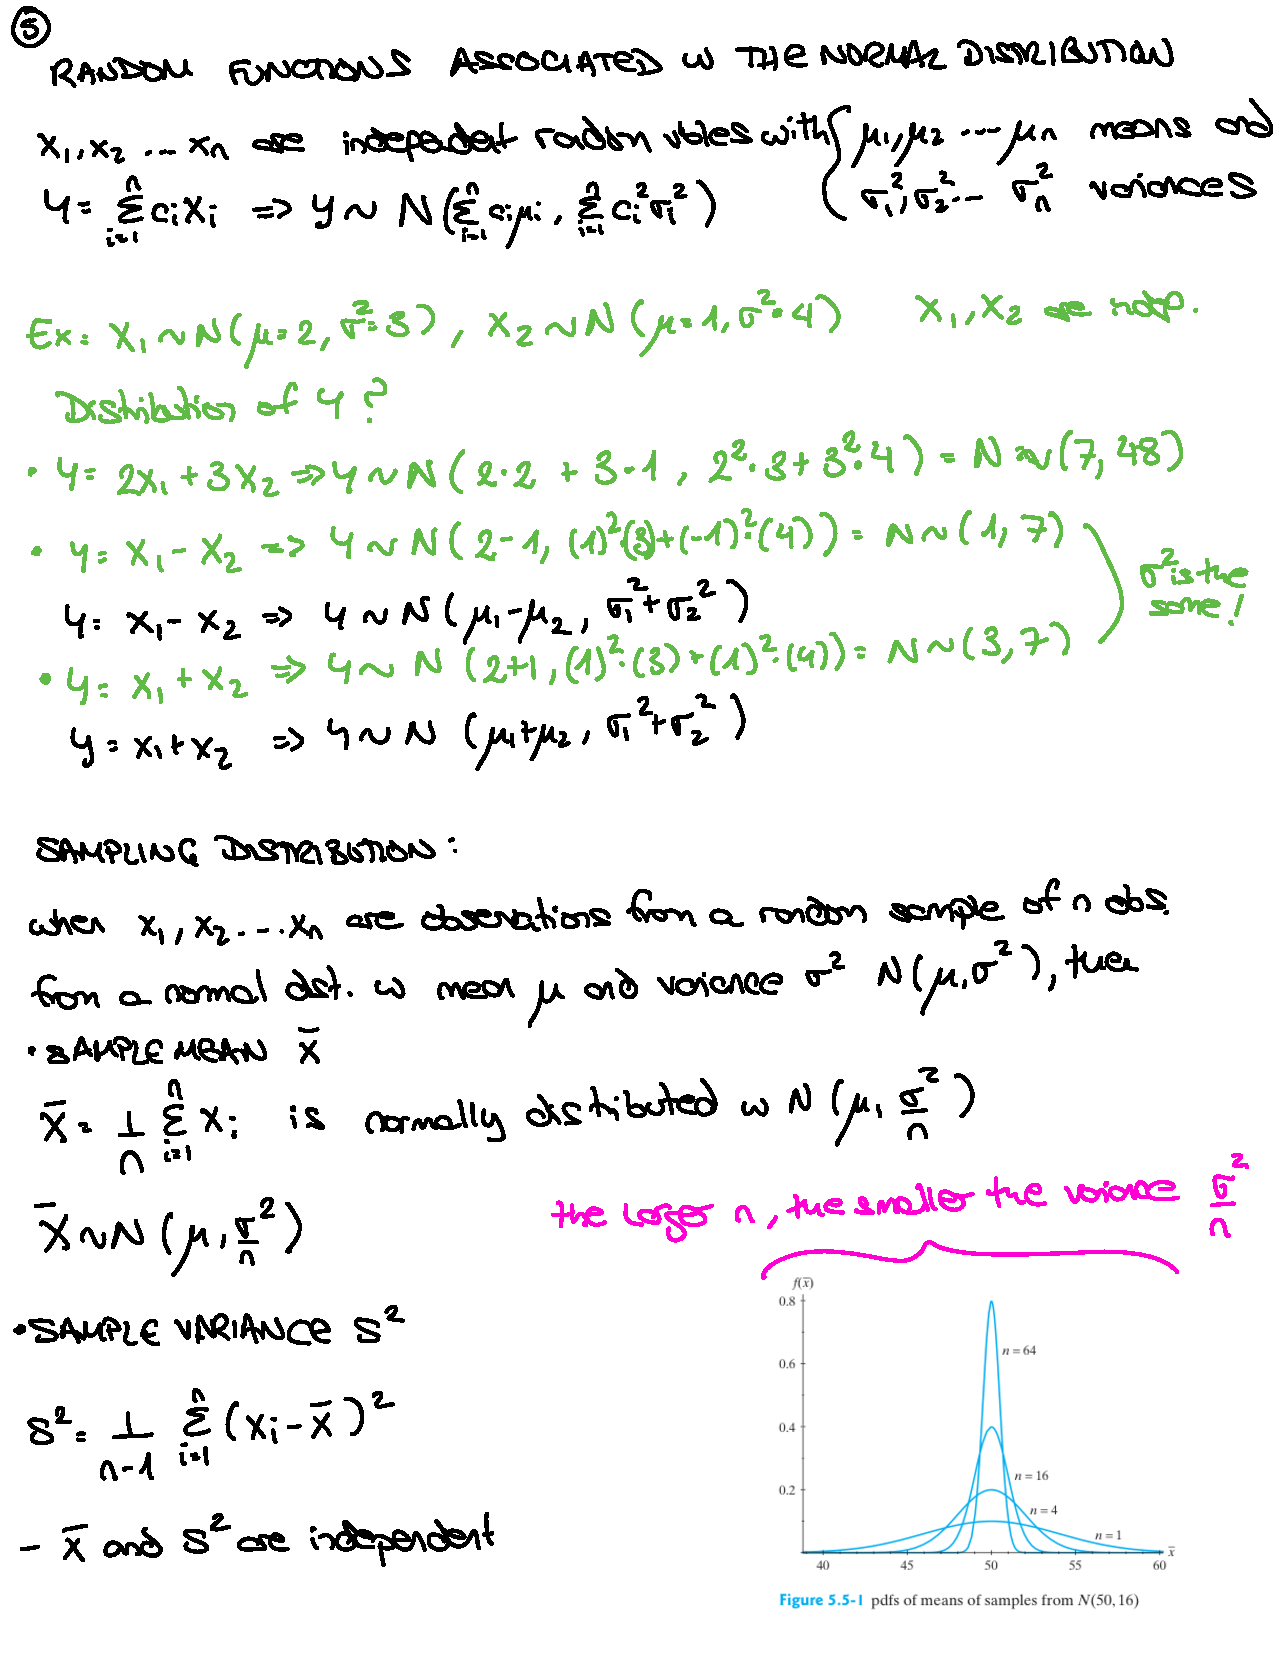
\includegraphics{/Users/annakawiecki/Documents/epi/workshops/akawiecki_pubs/pubs/DAG/notes screenshots/EPI 203 NOTES Jan 12, 2019hyp1.jpg}
\includegraphics{/Users/annakawiecki/Documents/epi/workshops/akawiecki_pubs/pubs/DAG/notes screenshots/EPI 203 NOTES Jan 12, 2019hyp2.jpg}

\hypertarget{significance-testing}{%
\subsubsection{significance testing}\label{significance-testing}}

\textbf{interpretation of the significance test}:

p-value: probability of observing a more extreme point estimate than
that observed in the sample if the \(H_0\) were true.

Reject the \(H_0\): probability of observing a more extreme point
estimate than that observed in the sample if the \(H_0\) were true is
less than the probability of the critical region (\(\alpha\) = 0.05) =
the smallest critical region (\(\alpha\)) that would lead us to reject
the \(H_0\) if it were true.

\textbf{MISinterpretation of the significance test}:

\begin{itemize}
\item
  p-value: probability of the observed data under the test hypothesis
  Incorrect because the p-value includes all other configurations of the
  data that result in a more extreme test statistic than that observed
  in the sample.
\item
  p-value: probability of the observed data would show as strong an
  association or stronger under the test hypothesis
\end{itemize}

\begin{figure}
\centering
\includegraphics{/Users/annakawiecki/Documents/epi/workshops/akawiecki_pubs/pubs/DAG/notes screenshots/EPI 203 NOTES Jan 12, 2019sig.jpg}
\caption{Hogg,Tannis,Zimmerman}
\end{figure}

\textbf{STATISTICAL ESTIMATION}

Epidemiological analysis is a measurement, not a decision-making,
problem. We want to estimate

\begin{itemize}
\item
  \textbf{the magnitude of the effect} = point estimate. The proximity
  of the measure of occurrence to the true value depends on sample size,
  bias, random error, etc\ldots{}
\item
  \textbf{the precision} of the estimation method = \textbf{statistical
  precision}: the inverse of the variance. Uncertainty of the point
  estimate. It depends on the random variability, the sample size,
  etc\ldots{}
\end{itemize}

\textbf{Interval estimation}: provides information on:

\begin{itemize}
\tightlist
\item
  the direction and magnitude of the association
\item
  the random variability in the point estimate.
\end{itemize}

\textbf{significance testing} reduce the information to a yes/no choice.
It provides the degree of consistency between the data and a single
hypothesis.

\hypertarget{systematic-error-bias}{%
\subsection{SYSTEMATIC ERROR = BIAS}\label{systematic-error-bias}}

\hypertarget{selection-bias}{%
\subsubsection{SELECTION BIAS}\label{selection-bias}}

Non-comparability of the exposed and unexposed groups induced by a
restriction in the analysis on certain level/s of a common effect of E
or O or variables correlated with E or O.

This can be caused by:

\begin{itemize}
\item
  unbalanced sampling fractions between the exposed and non-exposed
  population (see example below).
\item
  over-matching: when the cases and controls are matched on a factor
  that is not associated with the outcome but is associated with
  exposure.
\end{itemize}

The difference with confounding: confounding is due to unmeasured common
causes and selection bias is due to errors in the selection of the two
study groups that affects the internal validity.

\begin{itemize}
\item
  \textbf{non-response bias}: survey non-respondents may have different
  characteristics than those who do respond
\item
  \textbf{exclusion bias}: different eligibility criteria between cases
  and controls or the controls are selected from a different population
  than the cases Foor example, if the disease is very deadly and the
  information about the cases comes from proxies (relatives, friends)
  that are from a different population than the controls.

  \begin{itemize}
  \item
    \textbf{berkson's bias}: ``If the only way to cross the threshold is
    to score high, it is more common to score high on one item than on
    both. This general phenomenon is sometimes called Berkson's paradox
    . But it is easier to remember if we call it the
    \emph{selection-distortion effect}. Why do so many restaurants in
    good locations have bad food? The only way a restaurant with
    less-than-good food can survive is if it is in a nice location.
    Similarly, restaurants with excellent food can survive even in bad
    locations. Selection-distortion ruins your city.''(@mcelreath). In
    case-control studies that select cases from hospitals, often these
    cases are more likely to have concomitant diseases (hypertension,
    obesity) than the general population, which can lead to spurious
    associations.
  \item
    \textbf{incidence/prevalence bias}: Studies that select cases from
    hospitals are selecting for severe disease and having survived
    longer. To avoid this bias it's better to select incidence cases.
  \end{itemize}
\end{itemize}

\includegraphics{/Users/annakawiecki/Documents/epi/workshops/akawiecki_pubs/pubs/DAG/notes screenshots/EPI 207 notes irva_sel.jpg}

Selection bias does not depend only on exposure, it depends on the
sampling fraction of all the cells, that means it can also depend on
disease.

\includegraphics{epi_curious_files/figure-latex/dag selection bias-1.pdf}

\hypertarget{information-bias}{%
\subsubsection{INFORMATION BIAS}\label{information-bias}}

Bias caused by measurement errors. Individuals are categorized
incorrectly.

For continuous variables = \textbf{INFORMATION ERROR}

For categorical variables = \textbf{MISCLASSIFICATION}

\begin{itemize}
\item
  DIFFERENTIAL: the classification error depends on the actual values of
  other variables, that is, it varies between the study groups. The bias
  can be either towards or away from the \(H_0\).

  \begin{itemize}
  \item
    \textbf{recall bias}: memory of events may bary between cases and
    controls. Example: Outcome: congenital malformation; Exposure: any;
    mothers of cases may have a better memory of the exposure than
    mothers of controls.
  \item
    \textbf{detection/surveillance bias}: the diagnosis of the outcome
    may be earlier or better in monitored study groups than in the
    general population. Example: Outcome: emphysema; Exposure: smoking;
    smokers have more respoiratory issues and seek out medical care more
    often, therefore emphysema is detected earlier and more often in the
    exposed than in the unexposed.
  \item
    \textbf{observer bias}: there is a systematic difference in how data
    are collected between study participants belonging to different
    groups. Occurs when the interviewer is not blinded and when there is
    interviewer drift, that is, when the data collection procedure for
    the same interviewer changes over time.
  \end{itemize}
\item
  NON-DIFFERENTIAL: the classification error dos NOT depend on the
  actual values of other variables, and is due to a lack of accuracy in
  the data collection. This bias is usually towards the \(H_0\),
  diluting the magnitude of effect (RR and OR), but it can be away from
  the \(H_0\) if the exposure or outcome variables are non-binary, or if
  it's a dependent missclasification (depends on error in the
  classification of other variables).

  \begin{itemize}
  \tightlist
  \item
    \textbf{observer bias}: Example: surrogate interviews, where the
    information might be inaccurate.
  \end{itemize}

  NON-DIFFERENTIAL EXPOSURE MISSCLASIFICATION

  \begin{figure}
  \centering
  \includegraphics{/Users/annakawiecki/Documents/epi/workshops/akawiecki_pubs/pubs/DAG/notes screenshots/EPI 207 notes irvanondif.jpg}
  \caption{Modern Epidemiology}
  \end{figure}

  NON-DIFFERENTIAL DISEASE MISSCLASIFICATION

  \begin{figure}
  \centering
  \includegraphics{/Users/annakawiecki/Documents/epi/workshops/akawiecki_pubs/pubs/DAG/notes screenshots/EPI 207 notes irvadis.jpg}
  \caption{Modern Epidemiology}
  \end{figure}
\item
  DEPENDENT: the classification error depends on errors made measuring
  or classifying other variables.
\item
  INDEPENDENT: the classification error does NOT depend on errors made
  measuring or classifying other variables.
\end{itemize}

\hypertarget{confounding}{%
\subsubsection{CONFOUNDING}\label{confounding}}

The exposed and the unexposed in the study are not comparable, or
exchangeable, which is the ultimate source of the bias ( the unexposed
group is not the counterfactual of the exposed group)

A \textbf{CONFOUNDER} is a variable that is:

\begin{itemize}
\item
  associated with the outcome, conditional on the exposure (i.e.~in the
  exposed group) Example: smoking is a risk factor for cancer
\item
  associated with the exposure, conditional on the exposure (i.e.~in the
  exposed group) Example: smoking is associated with drinking coffee
\item
  not on the causal pathway between the exposure and the outcome.
  Example: smoking is not a result of drinking coffee
\end{itemize}

\hypertarget{difference-between-confouding-and-selection-bias}{%
\subsubsection{difference between confouding and selection
bias}\label{difference-between-confouding-and-selection-bias}}

\begin{itemize}
\item
  There is \textbf{confounding} when the association between exposure
  and outcome includes a noncausal component attributable to their
  having an uncontrolled common cause.
\item
  There is \textbf{selection bias} when the association between exposure
  and outcome includes a noncausal component attributable to restricting
  the analysis to certain level(s) of a common effect of exposure and
  outcome or, more generally, to conditioning on a common effect of
  variables correlated with exposure and outcome.
\end{itemize}

\hypertarget{methods-for-identifyingdetecting-confounding}{%
\subsubsection{methods for identifying/detecting
confounding}\label{methods-for-identifyingdetecting-confounding}}

The following methods are extracted from @Hernan2002

\textbf{Statistical criteria alone are insufficient to characterize
either confounding or selection bias}. The only method to reliably
identify a counfounder is to combine statistical associations from the
data with background knowledge about the causal network that links
exposure, outcome, and potential confounders.

\begin{itemize}
\tightlist
\item
  Methods relying on statistical associations that can easily be
  identified from the data:
\end{itemize}

\begin{enumerate}
\def\labelenumi{\arabic{enumi}.}
\item
  \textbf{automatic variable selection procedures}: i.e stepwise
  regression. It's based on including variables with ``significant''
  p-values. It assumes that all important confounders will be selected.
\item
  \textbf{change in effect estimate}: comparison of the effect estimates
  between adjusted and unadjusted effect estimates. It assumes that any
  variable substantially associated with an estimate change is worth
  adjusting for.
\end{enumerate}

We evaluate the effect measure of the exposure of interest: crude and
stratified by the possible confounder. If the stratum-specific effect
measures are similar to each other but different to the crude effect
measure and the relative change greater than 10\%, the variable is
selected as a confounder. This change can be evaluated on the
probability scale or transformed scale (exampe \(\beta\) coefficient or
OR for the exposure in a logistic model)

Example: Is the association causal or confounded by age?

\includegraphics{/Users/annakawiecki/Documents/epi/workshops/akawiecki_pubs/pubs/DAG/notes screenshots/strat example.png}

\includegraphics{/Users/annakawiecki/Documents/epi/workshops/akawiecki_pubs/pubs/DAG/notes screenshots/strat.png}

\begin{itemize}
\tightlist
\item
  Methods that combine statistical associations from the data with
  background knowledge:
\end{itemize}

\begin{enumerate}
\def\labelenumi{\arabic{enumi}.}
\setcounter{enumi}{2}
\tightlist
\item
  \textbf{check whether the variable meets the criteria of a
  confounder}: combines information from statistical associations and
  background knowledge. The presence of common causes, and therefore of
  confounding, can be represented by causal diagrams known as directed
  acyclic graphs (DAGs).
\end{enumerate}

\textbf{DAG = Directed Acyclic Graph}

DAGs are diagrams that link variables by arrows that represent direct
causal effects (protective or causative) of one variable on another.

There are only four types of variable relations that combine to form all
possible paths (from @mcelreath2020):

\begin{enumerate}
\def\labelenumi{\arabic{enumi})}
\item
  the \textbf{confounder} = \textbf{fork}: X ← Z → Y. This is the
  classic confounder: some variable Z is a common cause of X and Y,
  generating a correlation between them. If we condition on Z, then
  learning X tells us nothing about Y. X and Y are independent,
  conditional on Z.
\item
  the \textbf{pipe} = \textbf{intermediary}: X → Z → Y. The treatment X
  influences Z which influences Y. If we condition on Z, we block the
  path from X to Y. X and Y are independent, conditional on Z.
\item
  the \textbf{collider} = \textbf{common effect}: X → Z ← Y.
  Conditioning on Z, the collider variable, opens the path. X and Y are
  dependent, conditional on Z, however neither X nor Y has any causal
  influence on the other.
\item
  the \textbf{descendent} = \textbf{association?}: Z \(\to\) D.
  Descendent is a variable influenced by another variable. Conditioning
  on a descendent partly conditions on its parent. Conditioning on D
  will also condition, to a lesser extent, on Z because D has some
  information about Z.
\end{enumerate}

\textbf{Backdoor criterion}

Path: any series of variables you could walk through to get from one
variable to another, ignoring the directions of the arrows.

Blocking all confounding paths between some predictor X and some outcome
Y is known as shutting the backdoor, thus eliminating spurious
associations that are non-causal.

Example:

\includegraphics{epi_curious_files/figure-latex/confounder 1-1.pdf}

There are two paths connecting E and O:

\begin{enumerate}
\def\labelenumi{(\arabic{enumi})}
\item
  E → O
\item
  E ← C → O.
\end{enumerate}

Both of these paths create a statistical association between E and O.
But only the first path is causal. The second path is non-causal. If
only the second path existed, and we changed E, it would not change O.
Any causal influence of E on O operates only on the first path.

REMINDER:

\begin{itemize}
\item
  causal effect: The total causal effect is the sum of the direct and
  indirect effects: Example: age of marriage influences divorce in two
  ways.

  \begin{itemize}
  \item
    direct effect. A \(\to\) D Example: a direct effect would arise
    because younger people change faster than older people and are
    therefore more likely to grow incompatible with a partner.
  \item
    indirect effect. A \(\to\) M \(\to\) D Example: age of marriage has
    an indirect effect by influencing the marriage rate, which then
    influences divorce. If people get married earlier, then the marriage
    rate may rise, because there are more young people. Consider for
    example if an evil dictator forced everyone to marry at age 65.
    Since a smaller fraction of the population lives to 65 than to 25,
    forcing delayed marriage will also reduce the marriage rate. If
    marriage rate itself has any direct effect on divorce, maybe by
    making marriage more or less normative, then some of that direct
    effect could be the indirect effect of age at marriage.
  \end{itemize}
\end{itemize}

\includegraphics{epi_curious_files/figure-latex/dag1.3 ex1-1.pdf}

\begin{itemize}
\tightlist
\item
  spurious effect
\end{itemize}

\includegraphics{epi_curious_files/figure-latex/dag2 ex1-1.pdf}

\textbf{Do-operator}

do(E) closes the backdoor paths into E, as in a manipulative experiment.

P(O\textbar do(E)) defines a causal relationship because it tells us the
expected result of manipulating E on O

\begin{itemize}
\item
  Confounding: P(O\textbar E) \(\ne\) P(O\textbar do(E)). The
  relationship between the E and O when the backdoor paths are closed is
  not the same, indicating that there is confounding.
\item
  Conditional probability, non-causal: P(O\textbar E) \(\ne\)
  P(O\textbar not-E) doesn't close the backdoor, and therefore does not
  give a causal relationship.
\item
  Total causal relationship: if P(O\textbar do(E)) \(\ne\)
  P(O\textbar not-E), then E is the cause of O.
\item
  Direct causal relationship: might require closing more backdoor paths.
\end{itemize}

Examples from @Hernan2002

\includegraphics{/Users/annakawiecki/Documents/epi/workshops/akawiecki_pubs/pubs/DAG/notes screenshots/EPI 207 notes irva dag1.jpg}

\includegraphics{/Users/annakawiecki/Documents/epi/workshops/akawiecki_pubs/pubs/DAG/notes screenshots/EPI 207 notes irva dag2.jpg}

Example using all 3 methods of identifying confounders:

\includegraphics{/Users/annakawiecki/Documents/epi/workshops/akawiecki_pubs/pubs/DAG/notes screenshots/Screen Shot 2020-12-07 at 13.39.14.png}

\textbf{Steps to identify which variables are confounders and must be
controlled to obtain and unbiased causal effect estimate}:

\begin{enumerate}
\def\labelenumi{\arabic{enumi}.}
\item
  List all of the paths connecting E (the potential cause of interest)
  and O (the outcome).
\item
  Classify each path by whether it is open or closed. A path is open
  unless it contains a collider.
\item
  Classify each path by whether it is a backdoor path. A backdoor path
  has an arrow entering E.
\item
  If there are any open backdoor paths, decide which variable(s) to
  condition on to close it (if possible). To obtain a \textbf{sufficient
  set}, use the smallest set of confounders (preferable closer to the
  outcome)
\end{enumerate}

\begin{itemize}
\item
  Obtaining an unbiased estimate of the \textbf{total causal effect}
  requires measuring and adjusting for all confounders of the E \(\to\)
  O association
\item
  Obtaining an unbiased estimate of the \textbf{direct causal effect}
  requires measuring and adjusting for all confounders of both the

  \begin{itemize}
  \item
    E \(\to\) O association
  \item
    J \(\to\) O association
  \end{itemize}
\end{itemize}

\begin{enumerate}
\def\labelenumi{\arabic{enumi}.}
\tightlist
\item
  Example 1
\end{enumerate}

\includegraphics{epi_curious_files/figure-latex/dag1.4 ex1-1.pdf}

\begin{itemize}
\item
  To obtain the \textbf{total causal effect} we don't condition on C or
  J:

  \begin{itemize}
  \tightlist
  \item
    C is a confounder of the J \(\to\) O association but not the E
    \(\to\) O association, thanks to J which is a collider and blocks
    the path between C \(\to\) E, so it is unnecessary to control for C
  \end{itemize}
\end{itemize}

\includegraphics{epi_curious_files/figure-latex/adjust C ex-1.pdf}

\begin{itemize}
\tightlist
\item
  J is a \textbf{collider} of the E \(\to\) C association so if we
  condition on J we create a backdoor path between O \(\to\) E through
  C.
\end{itemize}

\includegraphics{epi_curious_files/figure-latex/adjust J ex-1.pdf}

\begin{itemize}
\tightlist
\item
  To obtain the \textbf{direct causal effect} we condition on both J and
  C, because we want only the
\end{itemize}

\includegraphics{epi_curious_files/figure-latex/adjust JC ex-1.pdf}

\begin{enumerate}
\def\labelenumi{\arabic{enumi}.}
\setcounter{enumi}{1}
\tightlist
\item
  Example 2
\end{enumerate}

\includegraphics{epi_curious_files/figure-latex/dag1.4 ex2-1.pdf}

\begin{itemize}
\item
  To obtain the \textbf{total causal effect} we condition on C but not
  J:

  \begin{itemize}
  \tightlist
  \item
    C is a confounder of the E \(\to\) O association so we must
    condition on it to obtain the unbiased total causal effect
  \end{itemize}
\end{itemize}

\includegraphics{epi_curious_files/figure-latex/adjust C ex2-1.pdf}

\begin{itemize}
\tightlist
\item
  To obtain the \textbf{direct causal effect} we condition on J. C is no
  longer a confounder because we block the path through J so it's no
  longer associated with O.
\end{itemize}

\includegraphics{epi_curious_files/figure-latex/adjust J ex2-1.pdf}

\begin{enumerate}
\def\labelenumi{\arabic{enumi}.}
\setcounter{enumi}{2}
\tightlist
\item
  Example 3.
\end{enumerate}

\includegraphics{epi_curious_files/figure-latex/dag1.5 ex-1.pdf}

\begin{itemize}
\tightlist
\item
  To obtain the total causal effect we condition on D
\end{itemize}

\includegraphics{epi_curious_files/figure-latex/adjust D ex-1.pdf}

\begin{itemize}
\tightlist
\item
  To obtain the total causal effect we condition on C, D, J
\end{itemize}

\includegraphics{epi_curious_files/figure-latex/adjust JCD ex-1.pdf}

\textbf{TESTABLE IMPLICATIONS}

Testable implications can be read off the diagrams using a graphical
criterion known as \textbf{d- separation} (Pearl, 1988). Each diagram
encodes causal assumptions, each corresponding to a missing arrow or a
missing double-arrow between a pair of variables.

DAGs imply that some variables are independent of others under certain
conditions, therefore the testable implications of a DAG are it's
\textbf{CONDITIONAL INDEPENDENCIES}.

\textbf{CONDITIONAL INDEPENDENCIES} describe which variables should be
associated with one another (or not) in the data, and which variables
become disassociated when we condition on some other set of variables.

Condition independencies are pairs of variables that are not associated,
once we condition on some set of other variables.

\textbf{Conditioning}: conditioning on a variable Z means learning its
value and then asking if X adds any additional information about Y. If
learning X doesn't give you any more information about Y, then we might
say that Y is independent of X conditional on Z. This conditioning
statement is sometimes written as: \(Y \!\perp\!\!\!\perp X|Z\)

\(X \not\!\perp\!\!\!\perp Y\) means ``not independent of''

\(X \!\perp\!\!\!\perp Y\) means ``independent of''

\textbf{Marginal and conditional assotiation}

\begin{figure}
\centering
\includegraphics{/Users/annakawiecki/Documents/epi/workshops/akawiecki_pubs/pubs/DAG/notes screenshots/EPI 207 notes irva ass.jpg}
\caption{Modern Epidemiology}
\end{figure}

\hypertarget{methods-for-controlling-confounding-obtaining-an-unbiased-estimate-of-the-causal-effect}{%
\subsubsection{methods for controlling confounding = obtaining an
unbiased estimate of the causal
effect}\label{methods-for-controlling-confounding-obtaining-an-unbiased-estimate-of-the-causal-effect}}

\textbf{DURING STUDY DESIGN}

Manipulation of the confounding factor in the study design removes the
influence of C on E: when we determine E, the C variable does not
influence E, thus blocking the non-causal path between E and O (E ← C →
O). Once the path is blocked, there is only one way for information to
go between E and O, and then measuring the association between E and O
would yield a useful measure of causal influence.

\begin{itemize}
\tightlist
\item
  \textbf{Randomization}: limits confounding by unmeasured factors
  probabilistically and accounts quantitavely for any residual
  confounding they produce.
\end{itemize}

Limitations: feasibility, ethics

\begin{itemize}
\tightlist
\item
  \textbf{Restriction}: the individuals in the study may be selected to
  have equal levels of the confounder.
\end{itemize}

Limitations: reduction of the number of available individuals, the
factor that is used for restriction can't be analyzed, possible residual
confounding if the restriction is insufficient.

\begin{itemize}
\tightlist
\item
  \textbf{Matching}: it does not control for confounding, but it
  increases the efficiency of the study that does control for
  confounding, as the confounding factor may still be controlled in the
  analysis.
\end{itemize}

Limitations: expensive, complicated logistics, the factor that is used
for matching can't be analyzed, as the variables must be collected
before participant enrollment

\textbf{DURING DATA ANALYSIS}

Conditioning on the confounding factor in the study analysis: adding C
to the model blocks the non-causal path E ← C → O.

Why? Think of this path in isolation, as a complete model.

\includegraphics{epi_curious_files/figure-latex/dag confounder condition ex1-1.pdf}

Once you learn C, also learning E will give you no additional
information about O.

Example: Suppose for example that C is the average wealth in a region.
Regions with high wealth have better schools, resulting in more
education (exposure E), as well as better paying jobs, resulting in
higher wages (outcome O). If you don't know the region a person lives
in, learning the person's education E will provide information about
their wages O, because E and O are correlated across regions. But after
you learn which region a person lives in, assuming there is no other
path between E and O, then learning E tells you nothing more about O.
This is the sense in which conditioning on C blocks the path --- it
makes E and O independent, conditional on C.

\begin{itemize}
\tightlist
\item
  \textbf{multivariate adjustment}: using regression, ANOVA, etc.. It
  can handle multiple covariates at the same time.
\end{itemize}

Limitations: unless background knowledge is included in the variable
selection, confounding can persist.

\begin{itemize}
\tightlist
\item
  \textbf{stratification}: the data is stratified by a confounder and
  the weighted averages of the effect measure (RR or OR) across strata
  is calculated and then compared to the crude estimate and to each
  other using the Cochran-Maentel-Haenszel estimate. \(OR_{EO}\) vs
  \(OR_{EO|C}\)
\end{itemize}

Limitations: can only be performed for few variables at a time

\begin{itemize}
\tightlist
\item
  \textbf{standarization}: re-weight the stratum-specific effect
  measures (RR, OR) so that the categories are comparable using a
  reference population from the data set r an external source.
\end{itemize}

Limitations: can only be performed for few variables at a time

\begin{itemize}
\tightlist
\item
  \textbf{inverse probability treatment}: creates a pseudo-population
  without confounding by re-weighting, yet the true exposure is not
  altered. It can be used for time-dependent confounding, when earlier
  exposure can influence later exposure.
\end{itemize}

\begin{figure}
\centering
\includegraphics{/Users/annakawiecki/Documents/epi/workshops/akawiecki_pubs/pubs/DAG/notes screenshots/EPI 207 notes irva inverse.jpg}
\caption{Modern Epidemiology}
\end{figure}

\hypertarget{confounding-example-from-mcelreath2020}{%
\subsubsection{confounding example from
@mcelreath2020}\label{confounding-example-from-mcelreath2020}}

We look into causal inference using a working example from Statistical
Rethinking: A Bayesian Course with Examples in R and Stan. Second
edition by Richard McElreath: Correlation between marriage rate (the
exposure) and divorce rate (the outcome).

\begin{Shaded}
\begin{Highlighting}[]
\CommentTok{# load data and copy }
\KeywordTok{library}\NormalTok{(rethinking) }
\KeywordTok{data}\NormalTok{(WaffleDivorce) }
\NormalTok{d <-}\StringTok{ }\NormalTok{WaffleDivorce}
\CommentTok{# standardize variables}
\NormalTok{d}\OperatorTok{$}\NormalTok{D <-}\StringTok{ }\KeywordTok{standardize}\NormalTok{( d}\OperatorTok{$}\NormalTok{Divorce )}
\NormalTok{d}\OperatorTok{$}\NormalTok{M <-}\StringTok{ }\KeywordTok{standardize}\NormalTok{( d}\OperatorTok{$}\NormalTok{Marriage )}
\NormalTok{d}\OperatorTok{$}\NormalTok{A <-}\StringTok{ }\KeywordTok{standardize}\NormalTok{( d}\OperatorTok{$}\NormalTok{MedianAgeMarriage )}
\end{Highlighting}
\end{Shaded}

\textbf{EXAMPLE 1}

There are three observed variables in play: divorce rate (D), marriage
rate (M), and the median age at marriage (A) in each State of the U.S.
Both marriage rates and median age at marriage are great predictors of
the divorce rate in a given State, but are these relationships causal?

The rate at which adults marry (M) is a great predictor of divorce rate.
But does marriage cause divorce? In a trivial sense it obviously does:
One cannot get a divorce without first getting married. But there's no
reason high marriage rate must cause more divorce. It's easy to imagine
high marriage rate indicating high cultural valuation of marriage and
therefore being associated with low divorce rate.

Age at marriage (A) is also a good predictor of divorce rate--- higher
age at marriage predicts less divorce. But there is no reason this has
to be causal, either, unless age at marriage is very late and the
spouses do not live long enough to get a divorce.

Age of marriage influences divorce in two ways:

\includegraphics{epi_curious_files/figure-latex/dag1.3 ex-1.pdf}

\begin{itemize}
\tightlist
\item
  direct effect: a direct effect would arise because younger people
  change faster than older people and are therefore more likely to grow
  incompatible with a partner.
\end{itemize}

\includegraphics{epi_curious_files/figure-latex/dag1.1 ex-1.pdf}

\begin{itemize}
\tightlist
\item
  indirect effect: age of marriage has an indirect effect by influencing
  the marriage rate, which then influences divorce. If people get
  married earlier, then the marriage rate may rise, because there are
  more young people. Consider for example if an evil dictator forced
  everyone to marry at age 65. Since a smaller fraction of the
  population lives to 65 than to 25, forcing delayed marriage will also
  reduce the marriage rate. If marriage rate itself has any direct
  effect on divorce, maybe by making marriage more or less normative,
  then some of that direct effect could be the indirect effect of age at
  marriage.
\end{itemize}

\includegraphics{epi_curious_files/figure-latex/dag1.2 ex-1.pdf}

To infer the strength of these different arrows, we need more than one
statistical model.

To obtain the \textbf{total effect} of of age at marriage on divorce
rate we condition on age at marriage.

The total causal effect is the sum of the direct and indirect effects

\includegraphics{epi_curious_files/figure-latex/dag ex1-1.pdf}

We assume that these variables are associated. If we look in the data
and find that any pair of variables are not associated, then something
is wrong with the DAG (assuming the data are correct). In these data,
all three pairs are in fact strongly associated. We can use cor to
measure simple correlations. Correlations are sometimes terrible
measures of association---many different patterns of association with
different implications can produce the same correlation. But they do
honest work in this case.

\begin{Shaded}
\begin{Highlighting}[]
\KeywordTok{cor}\NormalTok{(d}\OperatorTok{$}\NormalTok{D, d}\OperatorTok{$}\NormalTok{M)}
\end{Highlighting}
\end{Shaded}

\begin{verbatim}
## [1] 0.3737314
\end{verbatim}

\begin{Shaded}
\begin{Highlighting}[]
\KeywordTok{cor}\NormalTok{(d}\OperatorTok{$}\NormalTok{D, d}\OperatorTok{$}\NormalTok{A)}
\end{Highlighting}
\end{Shaded}

\begin{verbatim}
## [1] -0.5972392
\end{verbatim}

\begin{Shaded}
\begin{Highlighting}[]
\KeywordTok{cor}\NormalTok{(d}\OperatorTok{$}\NormalTok{M, d}\OperatorTok{$}\NormalTok{A)}
\end{Highlighting}
\end{Shaded}

\begin{verbatim}
## [1] -0.721096
\end{verbatim}

\begin{itemize}
\tightlist
\item
  \textbf{Model conditioning on A}
\end{itemize}

\(D_{i} ∼ Normal(\mu_{i}, \sigma)\)

\(\mu_{i} = \alpha + \beta_{A}A_{i}\)

\begin{Shaded}
\begin{Highlighting}[]
\NormalTok{m5}\FloatTok{.1}\NormalTok{ <-}\StringTok{ }\KeywordTok{quap}\NormalTok{(}
    \KeywordTok{alist}\NormalTok{(}
\NormalTok{        D }\OperatorTok{~}\StringTok{ }\KeywordTok{dnorm}\NormalTok{( mu , sigma ) ,}
\NormalTok{        mu <-}\StringTok{ }\NormalTok{a }\OperatorTok{+}\StringTok{ }\NormalTok{bA }\OperatorTok{*}\StringTok{ }\NormalTok{A ,}
\NormalTok{        a }\OperatorTok{~}\StringTok{ }\KeywordTok{dnorm}\NormalTok{( }\DecValTok{0}\NormalTok{ , }\FloatTok{0.2}\NormalTok{ ) ,}
        \CommentTok{#when βA = 1, a change of 1.2 years in median age at marriage is associated with a full standard deviation change in the outcome variable (divorce)}
        \CommentTok{#only 5% of plausible slopes more extreme than 1.}
\NormalTok{        bA }\OperatorTok{~}\StringTok{ }\KeywordTok{dnorm}\NormalTok{( }\DecValTok{0}\NormalTok{ , }\FloatTok{0.5}\NormalTok{ ) ,}
\NormalTok{        sigma }\OperatorTok{~}\StringTok{ }\KeywordTok{dexp}\NormalTok{( }\DecValTok{1}\NormalTok{ )}
\NormalTok{) , }\DataTypeTok{data =}\NormalTok{ d )}

\KeywordTok{precis}\NormalTok{(m5}\FloatTok{.1}\NormalTok{)}
\end{Highlighting}
\end{Shaded}

\begin{verbatim}
##                mean         sd       5.5%      94.5%
## a     -5.302872e-06 0.09738864 -0.1556512  0.1556406
## bA    -5.684310e-01 0.11001348 -0.7442538 -0.3926082
## sigma  7.884305e-01 0.07803712  0.6637121  0.9131489
\end{verbatim}

The outcome and the predictor are both standardized, the intercept α
should end up very close to zero.

What does the prior slope \(\beta_{A}\) imply? If \(\beta_{A}\) = 1,
that would imply that a change of one standard deviation in age at
marriage is associated likewise with a change of one standard deviation
in divorce. To know whether or not that is a strong relationship, you
need to know how big a standard deviation of age at marriage is:

\begin{Shaded}
\begin{Highlighting}[]
 \KeywordTok{sd}\NormalTok{( d}\OperatorTok{$}\NormalTok{MedianAgeMarriage )}
\end{Highlighting}
\end{Shaded}

\begin{verbatim}
## [1] 1.24363
\end{verbatim}

So when \(\beta_{A}\) = 1, a change of 1.2 years in median age at
marriage is associated with a full standard deviation change in the
outcome variable. That seems like an insanely strong relationship.

posterior for \(\beta_{A}\) is reliably negative, as seen:

\begin{Shaded}
\begin{Highlighting}[]
\CommentTok{# compute percentile interval of mean}
\NormalTok{A_seq <-}\StringTok{ }\KeywordTok{seq}\NormalTok{( }\DataTypeTok{from=}\OperatorTok{-}\DecValTok{3}\NormalTok{ , }\DataTypeTok{to=}\FloatTok{3.2}\NormalTok{ , }\DataTypeTok{length.out=}\DecValTok{30}\NormalTok{ )}
\NormalTok{mu <-}\StringTok{ }\KeywordTok{link}\NormalTok{( m5}\FloatTok{.1}\NormalTok{ , }\DataTypeTok{data=}\KeywordTok{list}\NormalTok{(}\DataTypeTok{A=}\NormalTok{A_seq) )}
\NormalTok{mu.mean <-}\StringTok{ }\KeywordTok{apply}\NormalTok{( mu , }\DecValTok{2}\NormalTok{, mean )}
\NormalTok{mu.PI <-}\StringTok{ }\KeywordTok{apply}\NormalTok{( mu , }\DecValTok{2}\NormalTok{ , PI )}
\CommentTok{# plot it all}
\KeywordTok{plot}\NormalTok{( D }\OperatorTok{~}\StringTok{ }\NormalTok{A , }\DataTypeTok{data=}\NormalTok{d , }\DataTypeTok{col=}\NormalTok{rangi2 )}
\KeywordTok{lines}\NormalTok{( A_seq , mu.mean , }\DataTypeTok{lwd=}\DecValTok{2}\NormalTok{ )}
\KeywordTok{shade}\NormalTok{( mu.PI , A_seq )}
\end{Highlighting}
\end{Shaded}

\includegraphics{epi_curious_files/figure-latex/5.5 ex-1.pdf}

Model m5.1, the regression of D on A, tells us only that the total
influence of age at marriage is strongly negative with divorce rate. The
``total'' here means we have to account for every path from A to D.
There are two such paths in this graph: A → D, a direct path,and A → M →
D, an indirect path.

\includegraphics{epi_curious_files/figure-latex/total effect dag ex-1.pdf}

In general, it is possible that a variable like A has no direct effect
at all on an outcome like D. It could still be associated with D
entirely through the indirect path. That type of relationship is known
as \textbf{mediation}.

As you'll see however, the indirect path does almost no work in this
case. How can we show that?

\begin{itemize}
\tightlist
\item
  \textbf{Model conditioning on M}
\end{itemize}

\(D_{i} ∼ Normal(\mu_{i}, \sigma)\)

\(\mu_{i} = \alpha + \beta_{M}M_{i}\)

\begin{Shaded}
\begin{Highlighting}[]
\NormalTok{m5}\FloatTok{.2}\NormalTok{ <-}\StringTok{ }\KeywordTok{quap}\NormalTok{(}
    \KeywordTok{alist}\NormalTok{(}
\NormalTok{        D }\OperatorTok{~}\StringTok{ }\KeywordTok{dnorm}\NormalTok{( mu , sigma ) ,}
\NormalTok{        mu <-}\StringTok{ }\NormalTok{a }\OperatorTok{+}\StringTok{ }\NormalTok{bM }\OperatorTok{*}\StringTok{ }\NormalTok{M ,}
\NormalTok{        a }\OperatorTok{~}\StringTok{ }\KeywordTok{dnorm}\NormalTok{( }\DecValTok{0}\NormalTok{ , }\FloatTok{0.2}\NormalTok{ ) ,}
\NormalTok{        bM }\OperatorTok{~}\StringTok{ }\KeywordTok{dnorm}\NormalTok{( }\DecValTok{0}\NormalTok{ , }\FloatTok{0.5}\NormalTok{ ) ,}
\NormalTok{        sigma }\OperatorTok{~}\StringTok{ }\KeywordTok{dexp}\NormalTok{( }\DecValTok{1}\NormalTok{ )}
\NormalTok{) , }\DataTypeTok{data =}\NormalTok{ d )}

\KeywordTok{precis}\NormalTok{(m5}\FloatTok{.2}\NormalTok{)}
\end{Highlighting}
\end{Shaded}

\begin{verbatim}
##                mean         sd       5.5%     94.5%
## a     -3.113195e-05 0.10824666 -0.1730302 0.1729679
## bM     3.500188e-01 0.12592804  0.1487615 0.5512762
## sigma  9.102682e-01 0.08986313  0.7666495 1.0538868
\end{verbatim}

\begin{Shaded}
\begin{Highlighting}[]
\CommentTok{# compute percentile interval of mean}
\NormalTok{M_seq <-}\StringTok{ }\KeywordTok{seq}\NormalTok{( }\DataTypeTok{from=}\OperatorTok{-}\DecValTok{3}\NormalTok{ , }\DataTypeTok{to=}\FloatTok{3.2}\NormalTok{ , }\DataTypeTok{length.out=}\DecValTok{30}\NormalTok{ )}
\NormalTok{mu <-}\StringTok{ }\KeywordTok{link}\NormalTok{( m5}\FloatTok{.2}\NormalTok{ , }\DataTypeTok{data=}\KeywordTok{list}\NormalTok{(}\DataTypeTok{M=}\NormalTok{M_seq) )}
\NormalTok{mu.mean <-}\StringTok{ }\KeywordTok{apply}\NormalTok{( mu , }\DecValTok{2}\NormalTok{, mean )}
\NormalTok{mu.PI <-}\StringTok{ }\KeywordTok{apply}\NormalTok{( mu , }\DecValTok{2}\NormalTok{ , PI )}
\CommentTok{# plot it all}
\KeywordTok{plot}\NormalTok{( D }\OperatorTok{~}\StringTok{ }\NormalTok{M , }\DataTypeTok{data=}\NormalTok{d , }\DataTypeTok{col=}\NormalTok{rangi2 )}
\KeywordTok{lines}\NormalTok{( M_seq , mu.mean , }\DataTypeTok{lwd=}\DecValTok{2}\NormalTok{ )}
\KeywordTok{shade}\NormalTok{( mu.PI , M_seq )}
\end{Highlighting}
\end{Shaded}

\includegraphics{epi_curious_files/figure-latex/5.6 ex-1.pdf}

This relationship isn't as strong as the one between A and D.

The pattern we see in the previous two models is symptomatic of a
situation in which only one of the predictor variables, A in this case,
has a causal impact on the outcome, D, even though both predictor
variables are strongly associated with the outcome.

We know from the model conditioning on M (m5.2) that marriage rate is
positively associated with divorce rate. But that isn't enough to tell
us that the path M → D is positive. It could be that the association
between M and D arises entirely from A's influence on both M and D. Like
this:

\includegraphics{epi_curious_files/figure-latex/dag mediation-1.pdf}

This DAG is also consistent with the posterior distributions of models
m5.1 and m5.2. Why? Because both M and D ``listen'' to A. They have
information from A. So when you inspect the association between D and M,
you pick up that common information that they both got from listening to
A.

So which is it? Is there a direct effect of marriage rate, or rather is
age at marriage just driving both, creating a spurious correlation
between marriage rate and divorce rate? To find out, we need to consider
carefully what each DAG implies.

\begin{enumerate}
\def\labelenumi{\arabic{enumi}.}
\tightlist
\item
  \textbf{M has influence on D}
\end{enumerate}

\includegraphics{epi_curious_files/figure-latex/dag1-1.pdf}

This DAG says:

\begin{enumerate}
\def\labelenumi{(\arabic{enumi})}
\tightlist
\item
  A directly influences D
\item
  M directly influences D
\item
  A directly influences M
\end{enumerate}

There are 3 causal assumptions that can be tested (one for every arrow).

Before we condition on anything, we assume everything is associated with
everything else.

The testable implications are:

\begin{enumerate}
\def\labelenumi{(\arabic{enumi})}
\tightlist
\item
  \(D \not\!\perp\!\!\!\perp A\) A not independent of D
\item
  \(D \not\!\perp\!\!\!\perp M\) M not independent of D
\item
  \(A \not\!\perp\!\!\!\perp M\) D not independent of A
\end{enumerate}

implied conditional independencies = none

\begin{Shaded}
\begin{Highlighting}[]
\NormalTok{DMA_dag1 <-}\StringTok{ }\KeywordTok{dagitty}\NormalTok{(}\StringTok{'dag\{ D <- A -> M -> D \}'}\NormalTok{)}

\KeywordTok{impliedConditionalIndependencies}\NormalTok{( DMA_dag1  )}
\end{Highlighting}
\end{Shaded}

\begin{enumerate}
\def\labelenumi{\arabic{enumi}.}
\setcounter{enumi}{1}
\tightlist
\item
  \textbf{M has no influence on D}
\end{enumerate}

\includegraphics{epi_curious_files/figure-latex/dag no DM-1.pdf}

In this DAG, it is still true that all three variable are associated
with one another. A is associated with D and M because it influences
them both. And D and M are associated with one another, because A
influences them both. They share a cause, and this leads them to be
correlated with one another through that cause.

There are 2 causal assumptions that can be tested (one for every arrow).

\begin{enumerate}
\def\labelenumi{(\arabic{enumi})}
\tightlist
\item
  A causes D
\end{enumerate}

\sout{(2) M causes D}

\begin{enumerate}
\def\labelenumi{(\arabic{enumi})}
\setcounter{enumi}{2}
\tightlist
\item
  A causes M
\end{enumerate}

But suppose we condition on A. All of the information in M that is
relevant to predicting D is in A. So once we've conditioned on A, M
tells us nothing more about D. So in the second DAG, a testable
implication is that D is independent of M, conditional on A. In other
words, \(D \!\perp\!\!\!\perp M|A\)

The testable implications are:

All 3 variables should be associated, before conditioning on anything:

\begin{enumerate}
\def\labelenumi{(\arabic{enumi})}
\item
  \(D \not\!\perp\!\!\!\perp A\) A not independent of D
\item
  \(D \not\!\perp\!\!\!\perp M\) M not independent of D
\item
  \(A \not\!\perp\!\!\!\perp M\) D not independent of A
\item
  \(D \!\perp\!\!\!\perp M|A\) D and M should be independent after
  conditioning on A.
\end{enumerate}

implied conditional independencies = D \emph{\textbar\textbar{}} M
\textbar{} A

\begin{Shaded}
\begin{Highlighting}[]
\NormalTok{DMA_dag2 <-}\StringTok{ }\KeywordTok{dagitty}\NormalTok{(}\StringTok{'dag\{ D <- A -> M \}'}\NormalTok{) }
\KeywordTok{impliedConditionalIndependencies}\NormalTok{( DMA_dag2  )}
\end{Highlighting}
\end{Shaded}

\begin{verbatim}
## D _||_ M | A
\end{verbatim}

\textbf{Test the difference between the two DAGs}

The only implication that differs between these DAGs is the last
one:\(D \!\perp\!\!\!\perp M|A\) D and M should be independent after
conditioning on A.

To test this implication, we need a statistical model that conditions on
A, so we can see whether that renders D independent of M. And that is
what multiple regression helps with. It can address a useful descriptive
question: \emph{Is there any additional value in knowing a variable,
once I already know all of the other predictor variables?}

So for example once you fit a multiple regression to predict divorce
using both marriage rate and age at marriage, the model addresses the
questions: (1) After I already know marriage rate, what additional value
is there in also knowing age at marriage? (2) After I already know age
at marriage, what additional value is there in also knowing marriage
rate?

The parameter estimates corresponding to each predictor are the (often
opaque) answers to these questions. The questions above are descriptive,
and the answers are also descriptive. It is only the derivation of the
testable implications above that give these descriptive results a causal
meaning. But that meaning is still dependent upon believing the DAG.

For each predictor, the parameter measures its conditional association
with the outcome.

\begin{itemize}
\tightlist
\item
  \textbf{Model conditioning on A and M}
\end{itemize}

\(D_{i} ∼ Normal(\mu_{i}, \sigma)\)

\(\mu_{i} = \alpha + \beta_{M}M_{i} + \beta_{A}A_{i}\)

\begin{Shaded}
\begin{Highlighting}[]
\NormalTok{m5}\FloatTok{.3}\NormalTok{ <-}\StringTok{ }\KeywordTok{quap}\NormalTok{(}
    \KeywordTok{alist}\NormalTok{(}
\NormalTok{        D }\OperatorTok{~}\StringTok{ }\KeywordTok{dnorm}\NormalTok{( mu , sigma ) ,}
\NormalTok{        mu <-}\StringTok{ }\NormalTok{a }\OperatorTok{+}\StringTok{ }\NormalTok{bM}\OperatorTok{*}\NormalTok{M }\OperatorTok{+}\StringTok{ }\NormalTok{bA}\OperatorTok{*}\NormalTok{A ,}
\NormalTok{        a }\OperatorTok{~}\StringTok{ }\KeywordTok{dnorm}\NormalTok{( }\DecValTok{0}\NormalTok{ , }\FloatTok{0.2}\NormalTok{ ) ,}
\NormalTok{        bM }\OperatorTok{~}\StringTok{ }\KeywordTok{dnorm}\NormalTok{( }\DecValTok{0}\NormalTok{ , }\FloatTok{0.5}\NormalTok{ ) ,}
\NormalTok{        bA }\OperatorTok{~}\StringTok{ }\KeywordTok{dnorm}\NormalTok{( }\DecValTok{0}\NormalTok{ , }\FloatTok{0.5}\NormalTok{ ) ,}
\NormalTok{        sigma }\OperatorTok{~}\StringTok{ }\KeywordTok{dexp}\NormalTok{( }\DecValTok{1}\NormalTok{ )}
\NormalTok{    ) , }\DataTypeTok{data =}\NormalTok{ d )}
\KeywordTok{precis}\NormalTok{( m5}\FloatTok{.3}\NormalTok{ )}
\end{Highlighting}
\end{Shaded}

\begin{verbatim}
##                mean         sd       5.5%      94.5%
## a      2.703037e-07 0.09707603 -0.1551460  0.1551465
## bM    -6.538085e-02 0.15077306 -0.3063453  0.1755836
## bA    -6.135135e-01 0.15098359 -0.8548145 -0.3722126
## sigma  7.851180e-01 0.07784339  0.6607092  0.9095268
\end{verbatim}

The posterior mean for marriage rate, bM, is now close to zero, with
plenty of probability of both sides of zero. The posterior mean for age
at marriage, bA, is essentially unchanged. It will help to visualize the
posterior distributions for all three models, focusing just on the slope
parameters βA and βM:

\begin{Shaded}
\begin{Highlighting}[]
\KeywordTok{plot}\NormalTok{(}\KeywordTok{coeftab}\NormalTok{(m5}\FloatTok{.1}\NormalTok{,m5}\FloatTok{.2}\NormalTok{,m5}\FloatTok{.3}\NormalTok{), }\DataTypeTok{par=}\KeywordTok{c}\NormalTok{(}\StringTok{"bA"}\NormalTok{,}\StringTok{"bM"}\NormalTok{))}
\end{Highlighting}
\end{Shaded}

\includegraphics{epi_curious_files/figure-latex/compare coefficients-1.pdf}

bA doesn't move, only grows a bit more uncertain, while bM is only
associated with divorce when age at marriage is missing from the model.
You can interpret these distributions as saying: \emph{Once we know
median age at marriage for a State, there is little or no additional
predictive power in also knowing the rate of marriage in that State},
which means \(D \!\perp\!\!\!\perp M|A\). D and M are independent after
conditioning on A, which corresponds to the second DAG.

\includegraphics{epi_curious_files/figure-latex/dag 5.3-1.pdf}

Note that this does not mean that there is no value in knowing marriage
rate. Consistent with the earlier DAG, if you didn't have access to
age-at-marriage data, then you'd definitely find value in knowing the
marriage rate. M is predictive but not causal. Assuming there are no
other causal variables missing from the model, this implies there is no
important direct causal path from marriage rate to divorce rate. The
association between marriage rate and divorce rate is spurious, caused
by the influence of age of marriage on both marriage rate and divorce
rate.

\textbf{EXAMPLE 2}

We're interested in the total causal effect of the number of Waffle
Houses on divorce rate in each State. Presumably, the naive correlation
between these two variables is spurious. What is the minimal adjustment
set that will block backdoor paths from Waffle House to divorce?

Let's make a graph:

\includegraphics{epi_curious_files/figure-latex/waffle dag-1.pdf}

\begin{verbatim}
## { A, M }
## { S }
\end{verbatim}

\includegraphics{epi_curious_files/figure-latex/waffle dag-2.pdf}

We could control for either A and M or for S alone. This DAG is
obviously not satisfactory---it assumes there are no unobserved
confounds, which is very unlikely for this sort of data. But we can
still learn something by analyzing it. While the data cannot tell us
whether a graph is correct, it can sometimes suggest how a graph is
wrong.

Inspecting implied conditional independencies, we can at least test some
of the features of a graph.

\begin{Shaded}
\begin{Highlighting}[]
 \KeywordTok{impliedConditionalIndependencies}\NormalTok{( dag6 )}
\end{Highlighting}
\end{Shaded}

\begin{verbatim}
## A _||_ W | S
## D _||_ S | A, M, W
## M _||_ W | S
\end{verbatim}

\begin{enumerate}
\def\labelenumi{\arabic{enumi})}
\item
  The median age of marriage should be independent of
  (\emph{\textbar\textbar{}}) Waffle Houses, conditioning on (\textbar)
  a State being in the south.
\item
  Divorce and being in the south should be independent when we
  simultaneously condition on all of median age of marriage, marriage
  rate, and Waffle Houses.
\item
  Marriage rate and Waffle Houses should be independent, conditioning on
  being in the south.
\end{enumerate}

\hypertarget{interaction-and-effect-measure-modification}{%
\subsection{INTERACTION and EFFECT MEASURE
MODIFICATION}\label{interaction-and-effect-measure-modification}}

An interaction occurs when the measure of association between a risk
factor and outcome depends on the level of another factor.

\hypertarget{difference-between-interaction-and-confounding}{%
\subsubsection{difference between interaction and
confounding}\label{difference-between-interaction-and-confounding}}

\begin{longtable}[]{@{}lll@{}}
\toprule
\begin{minipage}[b]{0.24\columnwidth}\raggedright
\strut
\end{minipage} & \begin{minipage}[b]{0.42\columnwidth}\raggedright
confounding\strut
\end{minipage} & \begin{minipage}[b]{0.26\columnwidth}\raggedright
interaction\strut
\end{minipage}\tabularnewline
\midrule
\endhead
\begin{minipage}[t]{0.24\columnwidth}\raggedright
origin\strut
\end{minipage} & \begin{minipage}[t]{0.42\columnwidth}\raggedright
property of distribution in source popuation\strut
\end{minipage} & \begin{minipage}[t]{0.26\columnwidth}\raggedright
biologic, sociologic\ldots{}\strut
\end{minipage}\tabularnewline
\begin{minipage}[t]{0.24\columnwidth}\raggedright
distribution of the 3d variable\strut
\end{minipage} & \begin{minipage}[t]{0.42\columnwidth}\raggedright
differs by exposure status\strut
\end{minipage} & \begin{minipage}[t]{0.26\columnwidth}\raggedright
can be statistically independent of exposure\strut
\end{minipage}\tabularnewline
\begin{minipage}[t]{0.24\columnwidth}\raggedright
does the 3d variable predic the outcome?\strut
\end{minipage} & \begin{minipage}[t]{0.42\columnwidth}\raggedright
yes\strut
\end{minipage} & \begin{minipage}[t]{0.26\columnwidth}\raggedright
not necessarily\strut
\end{minipage}\tabularnewline
\begin{minipage}[t]{0.24\columnwidth}\raggedright
stratum-specific measures\strut
\end{minipage} & \begin{minipage}[t]{0.42\columnwidth}\raggedright
similar across strata\strut
\end{minipage} & \begin{minipage}[t]{0.26\columnwidth}\raggedright
differ across strata\strut
\end{minipage}\tabularnewline
\begin{minipage}[t]{0.24\columnwidth}\raggedright
crude overall measure\strut
\end{minipage} & \begin{minipage}[t]{0.42\columnwidth}\raggedright
differ from stratum-specific measures\strut
\end{minipage} & \begin{minipage}[t]{0.26\columnwidth}\raggedright
falls between stratum-specific measures\strut
\end{minipage}\tabularnewline
\begin{minipage}[t]{0.24\columnwidth}\raggedright
summary adjusted measure\strut
\end{minipage} & \begin{minipage}[t]{0.42\columnwidth}\raggedright
makes sense\strut
\end{minipage} & \begin{minipage}[t]{0.26\columnwidth}\raggedright
not meaningful\strut
\end{minipage}\tabularnewline
\begin{minipage}[t]{0.24\columnwidth}\raggedright
testing\strut
\end{minipage} & \begin{minipage}[t]{0.42\columnwidth}\raggedright
cannot test\strut
\end{minipage} & \begin{minipage}[t]{0.26\columnwidth}\raggedright
can test\strut
\end{minipage}\tabularnewline
\begin{minipage}[t]{0.24\columnwidth}\raggedright
relationship to the other\strut
\end{minipage} & \begin{minipage}[t]{0.42\columnwidth}\raggedright
if a strong interaction exists, it makes no sense to discuss
confounding\strut
\end{minipage} & \begin{minipage}[t]{0.26\columnwidth}\raggedright
both may occur\strut
\end{minipage}\tabularnewline
\bottomrule
\end{longtable}

\hypertarget{difference-between-interaction-and-effect-measure-modification}{%
\subsubsection{difference between interaction and effect measure
modification}\label{difference-between-interaction-and-effect-measure-modification}}

Interaction, effect modification and effect heterogeneity sometimes are
used to mean the same thing.

Interaction Tables

\begin{itemize}
\tightlist
\item
  Risk of disease
\end{itemize}

\begin{longtable}[]{@{}lll@{}}
\toprule
& A no & A yes\tabularnewline
\midrule
\endhead
B no & Rab & RAb\tabularnewline
B yes & RaB & RAB\tabularnewline
\bottomrule
\end{longtable}

\begin{itemize}
\tightlist
\item
  \textbf{INTERACTION}: we are equally interested in the change in RR in
  the presence of A and B and the combination of A and B.
\end{itemize}

Relative Risk in Interaction

\begin{longtable}[]{@{}lll@{}}
\toprule
& A no & A yes\tabularnewline
\midrule
\endhead
B no & 1 & RAb/Rab\tabularnewline
B yes & RaB/Rab & RAB/Rab\tabularnewline
\bottomrule
\end{longtable}

\begin{itemize}
\tightlist
\item
  \textbf{EFFECT MODIFICATION}: we are interested in the change in RR of
  one of the variables in the presence of the other variable. Example:
  how does B change on different levels of A?
\end{itemize}

To obtain the relative risk measure, we divide the risk measures in the
presence of A by the referent within each level of B, thus we have 2
groups, one for each strata.

Relative Risk in effect modification

\begin{longtable}[]{@{}lll@{}}
\toprule
& A no & A yes\tabularnewline
\midrule
\endhead
B no & 1 & RaB/Rab\tabularnewline
B yes & 1 & RAB/RAb\tabularnewline
\bottomrule
\end{longtable}

\hypertarget{types-of-interaction}{%
\subsubsection{types of interaction}\label{types-of-interaction}}

\begin{itemize}
\item
  \textbf{synergism}: the additive measure of joint exposure is MORE
  THAN the sum of the measures of association between exposure and
  outcome for each exposure alone.
\item
  \textbf{antagonism}: the additive measure of joint exposure is LESS
  THAN the sum of the measures of association between the exposure and
  outcome for each exposure alone.
\end{itemize}

\hypertarget{types-of-interaction-effect}{%
\subsubsection{types of interaction
effect}\label{types-of-interaction-effect}}

\begin{itemize}
\item
  \textbf{additive}: Excess risk and linear regression are on the
  additive scale.
\item
  \textbf{multiplicative}: Relative risk, logistic, Poisson and
  porportional hazards models all assume factors act multiplicatively
  unless an interaction effect is included.
\end{itemize}

\begin{figure}
\centering
\includegraphics{/Users/annakawiecki/Documents/epi/workshops/akawiecki_pubs/pubs/DAG/notes screenshots/EPI 205 notes Sep 28, 2018 multadd.jpg}
\caption{Gordis}
\end{figure}

Example:

A logistic regression is on the additive scale when it's transformed:

\(logit(\hat{p_i}) = log(p_i/(1-p_i)) = log(ODDS) =\beta_0 +\beta_A x_A + \beta_B x_B + +\beta_{AB} x_A x_B\)

But a logistic regression is on the multiplicative scale when it's on
the original probability scale:

\(p_i/(1-p_i) = ODDS =e^{\beta_0 +\beta_A x_A + \beta_B x_B + +\beta_{AB} x_A x_B}\)

Is A and effect modifier of B? What is the effect of B versus no B?

\begin{itemize}
\item
  In the presence of A: \(x_A = 1\)

  \begin{itemize}
  \tightlist
  \item
    In the presence of B: \(x_B = 1\)
  \end{itemize}

  \(log(ODDS) =\beta_0 +\beta_A x_A + \beta_B x_B + \beta_{AB} x_A x_B\)

  \begin{itemize}
  \tightlist
  \item
    Not in the presence of B: \(x_B = 0\)
  \end{itemize}

  \(log(ODDS) =\beta_0 +\beta_A x_A\)
\end{itemize}

The difference in effect between B yes and B no is
\(\beta_B + \beta_{AB}\)

\((\beta_0 +\beta_A x_A + \beta_B x_B + \beta_{AB} x_A x_B) - (\beta_0 +\beta_A x_A ) = \beta_B + \beta_{AB}\)

\begin{itemize}
\item
  Not in the presence of A: \(x_A = 0\)

  \begin{itemize}
  \tightlist
  \item
    In the presence of B: \(x_B = 1\)
  \end{itemize}

  \(log(ODDS) =\beta_0 + \beta_B x_B\)

  \begin{itemize}
  \tightlist
  \item
    Not in the presence of B: \(x_B = 0\)
  \end{itemize}

  \(log(ODDS) =\beta_0\)
\end{itemize}

The difference in effect between B yes and B no is \(\beta_B\)

\((\beta_0 + \beta_B x_B) - (\beta_0) = \beta_B\)

There is effect modification if \(\beta_B \ne \beta_B+ \beta_{AB}\),
that is, if the presence of B has a different effect on the different
levels of A.

\hypertarget{methods-for-identifying-interactions}{%
\subsubsection{methods for identifying
interactions}\label{methods-for-identifying-interactions}}

\begin{enumerate}
\def\labelenumi{\arabic{enumi}.}
\item
  \textbf{automatic variable selection procedures}: i.e stepwise
  regression. It's based on including variables with ``significant''
  p-values. An interaction exists if an interaction coefficient has a
  ``significant p-value''.
\item
  \textbf{change in effect estimate}: comparison of the effect estimates
  between adjusted and unadjusted effect estimates.
\end{enumerate}

We evaluate the crude effect measure and the effect measure stratified
by the possible confounder or effect modifier. If the stratum-specific
effect measures are different from each other and the relative change
greater than 10\%, the variable is selected as a interaction.

If \(\beta_B\) in the presence of B but not A \(\ne\)
\(\beta_B+ \beta_{AB}\) in the presence of B and A, that is, if the
presence of B has a different effect on the different levels of A.

\begin{figure}
\centering
\includegraphics{/Users/annakawiecki/Documents/epi/workshops/akawiecki_pubs/pubs/DAG/notes screenshots/EPI 205 notes Sep 28, 2018 ex interaction.jpg}
\caption{Gordis}
\end{figure}

\hypertarget{interaction-example-1}{%
\subsubsection{interaction example 1}\label{interaction-example-1}}

Age adjusted rate ratios for lung cancer due to arsenic exposure.

\begin{longtable}[]{@{}llll@{}}
\toprule
& Unexposed area & Residentially exposed & Smelter worker\tabularnewline
\midrule
\endhead
Non smokers & 1 & 2.3 & 8.4\tabularnewline
Smokers- & 8.3 & 17.5 & 26.2\tabularnewline
\bottomrule
\end{longtable}

\begin{enumerate}
\def\labelenumi{\arabic{enumi}.}
\tightlist
\item
  \emph{Relative risk : multiplicative}
\end{enumerate}

\textbf{Does smoking interact multiplicatively with arsenic?}

\begin{longtable}[]{@{}llll@{}}
\toprule
& Unexposed area & Residentially exposed & Smelter worker\tabularnewline
\midrule
\endhead
Non smokers & 1 & 2.3 * 8.3 = 19 & 8.4 * 8.3 = 69\tabularnewline
Smokers- & 8.3 & 17.5 & 26.2\tabularnewline
\bottomrule
\end{longtable}

There is no multiplicative interaction between smoking and residential
arsenic exposure on lung cancer risk: \(2.3 * 8.3 = 19 \approx 17.5\)

There is an antagonistic multiplicative interaction between smoking and
smelter worker arsenic exposure on lung cancer risk:
\(8.4 * 8.3 = 69 \ne 26.2\)

\textbf{Is smoking an effect modifier of the arsenic relative risk?}

\begin{longtable}[]{@{}llll@{}}
\toprule
& Unexposed area & Residentially exposed & Smelter worker\tabularnewline
\midrule
\endhead
Non smokers & 1 & 2.3/1 & 8.4/1\tabularnewline
Smokers- & 8.3/8.3 & 17.5/8.3 & 26.2/8.3\tabularnewline
\bottomrule
\end{longtable}

\begin{longtable}[]{@{}llll@{}}
\toprule
& Unexposed area & Residentially exposed & Smelter worker\tabularnewline
\midrule
\endhead
Non smokers & 1 & 2.3 & 8.4\tabularnewline
Smokers- & 1 & 2.1 & 3.2\tabularnewline
\bottomrule
\end{longtable}

Smoking does not modify the effect of residential arsenic exposure on
lung cancer risk: \(2.3 \approx 2.1\)

Smoking does modify the effect of smelter workers' arsenic exposure on
lung cancer risk: this exposure has a much larger effect on non-smokers
that smokers: \(8.4 > 3.2\)

\begin{enumerate}
\def\labelenumi{\arabic{enumi}.}
\setcounter{enumi}{1}
\tightlist
\item
  \emph{Excess risk : additive}
\end{enumerate}

If we were looking at excess risk instead of relative risk, we would
look at the additive effect.

\textbf{Is smoking an effect modifier of the arsenic excess risk?}

\begin{longtable}[]{@{}llll@{}}
\toprule
& Unexposed area & Residentially exposed & Smelter worker\tabularnewline
\midrule
\endhead
Non smokers & 1 & 2.3-1 & 8.4-1\tabularnewline
Smokers- & 8.3 & 17.5-8.3 & 26.2-8.3\tabularnewline
\bottomrule
\end{longtable}

\begin{longtable}[]{@{}llll@{}}
\toprule
& Unexposed area & Residentially exposed & Smelter worker\tabularnewline
\midrule
\endhead
Non smokers & 1 & 1.3 & 7.4\tabularnewline
Smokers- & 8.3 & 9.2 & 17.9\tabularnewline
\bottomrule
\end{longtable}

Smoking does modify the effect of residential arsenic exposure on lung
cancer excess risk synergistically: \(1.3 < 9.2\)

Smoking does modify the effect of smelter workers' arsenic exposure on
lung cancer excess risk synergistically: \(7.4 < 17.9\)

\textbf{Does smoking interact additively with arsenic?}

\begin{longtable}[]{@{}llll@{}}
\toprule
& Unexposed area & Residentially exposed & Smelter worker\tabularnewline
\midrule
\endhead
Non smokers & 1 & 2.3-1 & 8.4-1\tabularnewline
Smokers- & 8.3-1 & 17.5-1 & 26.2-1\tabularnewline
\bottomrule
\end{longtable}

\begin{longtable}[]{@{}llll@{}}
\toprule
& Unexposed area & Residentially exposed & Smelter worker\tabularnewline
\midrule
\endhead
Non smokers & 1 & 1.3 & 7.4\tabularnewline
Smokers- & 7.3 & 16.5 & 25.2\tabularnewline
\bottomrule
\end{longtable}

There is additive interaction between smoking and residential arsenic
exposure on lung cancer risk: \(1.3 + 7.3 = 8.6 \ne 16.5\)

There is no additive interaction between smoking and smelter worker
arsenic exposure on lung cancer risk: \(7.4 + 16.5 = 23.9 \approx 25.2\)

\hypertarget{interaction-example-from-mcelreath2020-chapter-8}{%
\subsubsection{interaction example from @mcelreath2020 Chapter
8}\label{interaction-example-from-mcelreath2020-chapter-8}}

Africa is geographically special, in a puzzling way: Bad geography tends
to be related to bad economies outside of Africa, but African economies
may actually benefit from bad geography. To appreciate the puzzle, look
at regressions of terrain ruggedness---a particular kind of bad
geography---against economic performance (log GDP136 per capita in the
year 2000), both inside and outside of Africa. The variable rugged is a
Terrain Ruggedness Index137 that quantifies the topographic
heterogeneity of a landscape. The outcome variable here is the logarithm
of real gross domestic product per capita, from the year 2000,
rgdppc\_2000. We use the logarithm of it, because the logarithm of GDP
is the magnitude of GDP.

\begin{Shaded}
\begin{Highlighting}[]
\KeywordTok{library}\NormalTok{(rethinking) }
\KeywordTok{data}\NormalTok{(rugged)}
\NormalTok{d <-}\StringTok{ }\NormalTok{rugged}

\CommentTok{# make the log version of criterion}
\NormalTok{d <-}\StringTok{ }
\StringTok{  }\NormalTok{d }\OperatorTok
\StringTok{  }\KeywordTok{mutate}\NormalTok{(}\DataTypeTok{log_gdp =} \KeywordTok{log}\NormalTok{(rgdppc_}\DecValTok{2000}\NormalTok{))}

\CommentTok{# extract countries with GDP data}
\NormalTok{dd <-}
\StringTok{  }\NormalTok{d }\OperatorTok
\StringTok{  }\KeywordTok{filter}\NormalTok{(}\KeywordTok{complete.cases}\NormalTok{(rgdppc_}\DecValTok{2000}\NormalTok{)) }\OperatorTok\StringTok{ }
\StringTok{  }\CommentTok{# re-scale variables}
\StringTok{  }\KeywordTok{mutate}\NormalTok{(}\DataTypeTok{log_gdp_std =}\NormalTok{ log_gdp }\OperatorTok{/}\StringTok{ }\KeywordTok{mean}\NormalTok{(log_gdp), }
         \DataTypeTok{rugged_std  =}\NormalTok{ rugged }\OperatorTok{/}\StringTok{ }\KeywordTok{max}\NormalTok{(rugged))}
\end{Highlighting}
\end{Shaded}

\includegraphics{epi_curious_files/figure-latex/africa plot-1.pdf}

If this relationship is at all causal, it may be because rugged regions
of Africa were pro- tected against the Atlantic and Indian Ocean slave
trades. Slavers preferred to raid easily accessed settlements, with easy
routes to the sea. Those regions that suffered under the slave trade
understandably continue to suffer economically, long after the decline
of slave-trading markets. However, an outcome like GDP has many
influences, and is furthermore a strange measure of economic activity.
And ruggedness is correlated with other geographic features, like
coastlines, that also influence the economy. So it is hard to be sure
what's going on here.

The causal hypothesis, in DAG form, might be (where R is terrain
ruggedness, G is GDP, C is continent):
\includegraphics{epi_curious_files/figure-latex/dag2 africa-1.pdf} R and
C both influence G. This could mean that they are independent influences
or rather that they interact (one moderates the influence of the other).
The DAG does not display an interaction. That's because DAGs do not
specify how variables combine to influence other variables. The DAG
above implies only that there is some function that uses R and C to
generate G. In typical notation, G = f(R, C).

So we need a statistical approach to judge different propositions for
f(R, C).

So we need a statistical approach to judge different propositions for
f(R, C). How do we make a model that produces the conditionality in
Figure 8.2? We could cheat by splitting the data into two data frames,
one for Africa and one for all the other continents. But it's not a good
idea to split the data in this way. Here are four reasons:

\begin{enumerate}
\def\labelenumi{\arabic{enumi}.}
\item
  First, there are usually some parameters, such as σ, that the model
  says do not depend in any way upon continent. By splitting the data
  table, you are hurting the accuracy of the es- timates for these
  parameters, because you are essentially making two less-accurate
  estimates instead of pooling all of the evidence into one estimate. In
  effect, you have accidentally as- sumed that variance differs between
  African and non-African nations. Now, there's nothing wrong with that
  sort of assumption. But you want to avoid accidental assumptions.
\item
  Second, in order to acquire probability statements about the variable
  you used to split the data, cont\_africa in this case, you need to
  include it in the model. Otherwise, you have a weak statistical
  argument. Isn't there uncertainty about the predictive value of
  distinguishing between African and non-African nations? Of course
  there is. Unless you analyze all of the data in a single model, you
  can't easily quantify that uncertainty. If you just let the posterior
  distribution do the work for you, you'll have a useful measure of that
  uncertainty.
\item
  Third, we may want to use information criteria or another method to
  compare models. In order to compare a model that treats all continents
  the same way to a model that allows different slopes in different
  continents, we need models that use all of the same data (as explained
  in Chapter 7). This means we can't split the data for two separate
  models. We have to let a single model internally split the data.
\item
  Fourth, once you begin using multilevel models (Chapter 13), you'll
  see that there are advantages to borrowing information across
  categories like ``Africa'' and ``not Africa.'' This is especially true
  when sample sizes vary across categories, such that overfitting risk
  is higher within some categories. In other words, what we learn about
  ruggedness outside of Africa should have some effect on our estimate
  within Africa, and visa versa. Multilevel models (Chapter 13) borrow
  information in this way, in order to improve estimates in all
  categories. When we split the data, this borrowing is impossible.
\end{enumerate}

We look at the different possibilities to model the association between
log(GDP) and ruggedness

\begin{enumerate}
\def\labelenumi{\arabic{enumi}.}
\tightlist
\item
  m8.1 \textbf{ignoring continent}.
\end{enumerate}

Fit a single model to all the data, ignoring continent.

\(log(y_i) \sim N(\mu_i, \sigma)\)

\(\mu_i = \alpha_0 + \beta (r_i - \bar{r})\)

\begin{Shaded}
\begin{Highlighting}[]
\NormalTok{m8}\FloatTok{.1}\NormalTok{ <-}\StringTok{ }\KeywordTok{quap}\NormalTok{(}
    \KeywordTok{alist}\NormalTok{(}
\NormalTok{        log_gdp_std }\OperatorTok{~}\StringTok{ }\KeywordTok{dnorm}\NormalTok{( mu , sigma ) ,}
\NormalTok{        mu <-}\StringTok{ }\NormalTok{a }\OperatorTok{+}\StringTok{ }\NormalTok{b}\OperatorTok{*}\NormalTok{( rugged_std }\OperatorTok{-}\StringTok{ }\FloatTok{0.215}\NormalTok{ ) ,}
\NormalTok{        a }\OperatorTok{~}\StringTok{ }\KeywordTok{dnorm}\NormalTok{( }\DecValTok{1}\NormalTok{ , }\FloatTok{0.1}\NormalTok{ ) ,}
\NormalTok{        b }\OperatorTok{~}\StringTok{ }\KeywordTok{dnorm}\NormalTok{( }\DecValTok{0}\NormalTok{ , }\FloatTok{0.3}\NormalTok{ ) ,}
\NormalTok{        sigma }\OperatorTok{~}\StringTok{ }\KeywordTok{dexp}\NormalTok{(}\DecValTok{1}\NormalTok{)}
\NormalTok{    ) , }\DataTypeTok{data=}\NormalTok{dd )}

 \KeywordTok{precis}\NormalTok{( m8}\FloatTok{.1}\NormalTok{ )}
\end{Highlighting}
\end{Shaded}

\begin{verbatim}
##              mean          sd        5.5%      94.5%
## a     1.000000079 0.010412512  0.98335887 1.01664128
## b     0.002001904 0.054796238 -0.08557307 0.08957688
## sigma 0.136504552 0.007397121  0.12468252 0.14832658
\end{verbatim}

\includegraphics{epi_curious_files/figure-latex/m8.1 plot-1.pdf}

Really no overall association between terrain ruggedness and log GDP.

Next we'll see how to split apart the continents.

\begin{enumerate}
\def\labelenumi{\arabic{enumi}.}
\setcounter{enumi}{1}
\tightlist
\item
  m8.2 \textbf{adding indicator variable for African nations}
\end{enumerate}

The first thing to realize is that just in- cluding an indicator
variable for African nations, cont\_africa here, won't reveal the re-
versed slope. It's worth fitting this model to prove it to yourself,
though.

\(log(y_i) \sim N(\mu_i, \sigma)\)

\(\mu_i = \alpha_0 + \beta (r_i - \bar{r}) + \gamma A_i\)

where \(A_i\) is cont\_africa, a 0/1 indicator variable.

The problem here, and in general, is that we need a prior for
\(\gamma\). Okay, we can do priors. But what that prior will necessarily
do is tell the model that \(\mu_i\) for a nation in Africa is more
uncertain, before seeing the data, than \(\mu_i\) outside Africa. And
that makes no sense.

There is a simple solution: Nations in Africa will get one intercept and
those outside Africa another.

\(log(y_i) \sim N(\mu_i, \sigma)\)

\(\mu_i = \alpha_{CID[i]} + \beta (r_i - \bar{r})\)

where cid is an index variable, continent ID. It takes the value 1 for
African nations and 2 for all other nations. This means there are two
parameters, \(\alpha_{1}\) and \(\alpha_{2}\) one for each unique index
value. The notation cid{[}i{]} just means the value of cid on row i.
Using this approach, instead of the conventional approach of adding
another term with the 0/1 indicator variable, doesn't force us to say
that the mean for Africa is inherently less certain than the mean for
all other continents.

\begin{Shaded}
\begin{Highlighting}[]
\CommentTok{#make variable to index Africa (1) or not (2)}
\NormalTok{dd}\OperatorTok{$}\NormalTok{cid <-}\StringTok{ }\KeywordTok{ifelse}\NormalTok{( dd}\OperatorTok{$}\NormalTok{cont_africa}\OperatorTok{==}\DecValTok{1}\NormalTok{ , }\DecValTok{1}\NormalTok{ , }\DecValTok{2}\NormalTok{ )}

\NormalTok{m8}\FloatTok{.2}\NormalTok{ <-}\StringTok{ }\KeywordTok{quap}\NormalTok{( }\KeywordTok{alist}\NormalTok{(}
\NormalTok{log_gdp_std }\OperatorTok{~}\StringTok{ }\KeywordTok{dnorm}\NormalTok{( mu , sigma ) ,}
\NormalTok{mu <-}\StringTok{ }\NormalTok{a[cid] }\OperatorTok{+}\StringTok{ }\NormalTok{b}\OperatorTok{*}\NormalTok{( rugged_std }\OperatorTok{-}\StringTok{ }\FloatTok{0.215}\NormalTok{ ) , a[cid] }\OperatorTok{~}\StringTok{ }\KeywordTok{dnorm}\NormalTok{( }\DecValTok{1}\NormalTok{ , }\FloatTok{0.1}\NormalTok{ ) ,}
\NormalTok{b }\OperatorTok{~}\StringTok{ }\KeywordTok{dnorm}\NormalTok{( }\DecValTok{0}\NormalTok{ , }\FloatTok{0.3}\NormalTok{ ) ,}
\NormalTok{sigma }\OperatorTok{~}\StringTok{ }\KeywordTok{dexp}\NormalTok{( }\DecValTok{1}\NormalTok{ )}
\NormalTok{) , }\DataTypeTok{data=}\NormalTok{dd )}

\KeywordTok{precis}\NormalTok{( m8}\FloatTok{.2}\NormalTok{ , }\DataTypeTok{depth=}\DecValTok{2}\NormalTok{ )}
\end{Highlighting}
\end{Shaded}

\begin{verbatim}
##              mean          sd       5.5%      94.5%
## a[1]   0.88041284 0.015937003  0.8549424 0.90588325
## a[2]   1.04916425 0.010185554  1.0328858 1.06544274
## b     -0.04651347 0.045686725 -0.1195297 0.02650274
## sigma  0.11238738 0.006091077  0.1026527 0.12212209
\end{verbatim}

The parameter a{[}1{]} is the intercept for African nations. It seems
reliably lower than a{[}2{]}.

Now to compare these models, using WAIC:

\begin{verbatim}
##           WAIC       SE    dWAIC      dSE    pWAIC       weight
## m8.2 -252.2687 15.30518  0.00000       NA 4.258517 1.000000e+00
## m8.1 -188.7544 13.29153 63.51424 15.14616 2.690177 1.614571e-14
\end{verbatim}

m8.2 gets all the model weight. And while the standard error of the
difference in WAIC is 15, the difference itself is 64. So the continent
variable seems to be picking up some important association in the
sample.

Let's plot the posterior predictions for m8.2, so you can see how,
despite it's predictive superiority to m8.1, it still doesn't manage
different slopes inside and outside of Africa. African nations are shown
in blue, while nations outside Africa are shown in gray. What you've
ended up with here is a rather weak negative relationship between
economic development and ruggedness. The African nations do have lower
overall economic development, and so the blue regression line is below,
but parallel to, the black line. All including a dummy variable for
African nations has done is allow the model to predict a lower mean for
African nations. It can't do anything to the slope of the line. The fact
that WAIC tells you that the model with the dummy variable is hugely
better only indicates that African nations on average do have lower GDP.

\includegraphics{/Users/annakawiecki/Documents/epi/workshops/akawiecki_pubs/pubs/DAG/notes screenshots/Screen Shot 2020-12-08 at 16.27.33.png}

\begin{enumerate}
\def\labelenumi{\arabic{enumi}.}
\setcounter{enumi}{2}
\tightlist
\item
  m8.3 \textbf{adding interaction variable for African nations}
\end{enumerate}

How can you recover the change in slope you saw at the start of this
section? You need a proper interaction effect. This just means we also
make the slope conditional on continent.

And again, there is a conventional approach to specifying an interaction
that uses an indica- tor variable and a new interaction parameter. It
would look like this:

\(log(y_i) \sim N(\mu_i, \sigma)\)

\(\mu_i = \alpha_{CID[i]} + (\beta + \gamma A_i) (r_i - \bar{r})= \alpha_{CID[i]} +\beta(r_i - \bar{r})+ \gamma A_i(r_i - \bar{r})\)

where Ai is a 0/1 indicator for African nations. This is equivalent to
our index approach, but it is much harder to state sensible priors. Any
prior we put on γ makes the slope inside Africa more uncertain than the
slope outside Africa. And again that makes no sense. But in the indexing
approach, we can easily assign the same prior to the slope, no matter
which continent.

\(log(y_i) \sim N(\mu_i, \sigma)\)

\(\mu_i = \alpha_{CID[i]} + \beta_{CID[i]}(r_i - \bar{r})\)

\begin{Shaded}
\begin{Highlighting}[]
\NormalTok{m8}\FloatTok{.3}\NormalTok{ <-}\StringTok{ }\KeywordTok{quap}\NormalTok{(}
    \KeywordTok{alist}\NormalTok{(}
\NormalTok{        log_gdp_std }\OperatorTok{~}\StringTok{ }\KeywordTok{dnorm}\NormalTok{( mu , sigma ) ,}
\NormalTok{        mu <-}\StringTok{ }\NormalTok{a[cid] }\OperatorTok{+}\StringTok{ }\NormalTok{b[cid]}\OperatorTok{*}\NormalTok{( rugged_std }\OperatorTok{-}\StringTok{ }\FloatTok{0.215}\NormalTok{ ) ,}
\NormalTok{        a[cid] }\OperatorTok{~}\StringTok{ }\KeywordTok{dnorm}\NormalTok{( }\DecValTok{1}\NormalTok{ , }\FloatTok{0.1}\NormalTok{ ) ,}
\NormalTok{        b[cid] }\OperatorTok{~}\StringTok{ }\KeywordTok{dnorm}\NormalTok{( }\DecValTok{0}\NormalTok{ , }\FloatTok{0.3}\NormalTok{ ) ,}
\NormalTok{        sigma }\OperatorTok{~}\StringTok{ }\KeywordTok{dexp}\NormalTok{( }\DecValTok{1}\NormalTok{ )}
\NormalTok{) , }\DataTypeTok{data=}\NormalTok{dd )}

\KeywordTok{precis}\NormalTok{( m8}\FloatTok{.3}\NormalTok{ , }\DataTypeTok{depth=}\DecValTok{2}\NormalTok{ )}
\end{Highlighting}
\end{Shaded}

\begin{verbatim}
##             mean          sd       5.5%       94.5%
## a[1]   0.8865639 0.015675695  0.8615111  0.91161667
## a[2]   1.0505698 0.009936606  1.0346892  1.06645039
## b[1]   0.1325054 0.074204443  0.0139124  0.25109846
## b[2]  -0.1425767 0.054749403 -0.2300768 -0.05507653
## sigma  0.1094941 0.005935299  0.1000084  0.11897987
\end{verbatim}

The slope is essentially reversed inside Africa, 0.13 instead of −0.14.

How much does allowing the slope to vary improve expected prediction?
Let's use PSIS to compare this new model to the previous two. You could
use WAIC here as well. It'll give almost identical results.

\begin{verbatim}
##           PSIS       SE    dPSIS       dSE    pPSIS       weight
## m8.3 -258.9122 15.26994  0.00000        NA 5.248904 9.731544e-01
## m8.2 -251.7313 15.27774  7.18088  6.563466 4.462810 2.684562e-02
## m8.1 -188.7363 13.28687 70.17592 15.393216 2.681052 5.619209e-16
\end{verbatim}

Model family m8.3 has more than 95\% of the weight. That's very strong
support for including the interaction effect, if prediction is our goal.
But the modicum of weight given to m8.2 suggests that the posterior
means for the slopes in m8.3 are a little overfit. And the standard
error of the difference in PSIS between the top two models is almost the
same as the difference itself.

\begin{Shaded}
\begin{Highlighting}[]
\CommentTok{# plot Africa - cid=1}
\NormalTok{d.A1 <-}\StringTok{ }\NormalTok{dd[ dd}\OperatorTok{$}\NormalTok{cid}\OperatorTok{==}\DecValTok{1}\NormalTok{ , ]}
\KeywordTok{plot}\NormalTok{( d.A1}\OperatorTok{$}\NormalTok{rugged_std , d.A1}\OperatorTok{$}\NormalTok{log_gdp_std , }\DataTypeTok{pch=}\DecValTok{16}\NormalTok{ , }\DataTypeTok{col=}\NormalTok{rangi2 ,}
    \DataTypeTok{xlab=}\StringTok{"ruggedness (standardized)"}\NormalTok{ , }\DataTypeTok{ylab=}\StringTok{"log GDP (as proportion of mean)"}\NormalTok{ ,}
    \DataTypeTok{xlim=}\KeywordTok{c}\NormalTok{(}\DecValTok{0}\NormalTok{,}\DecValTok{1}\NormalTok{) )}
\NormalTok{mu <-}\StringTok{ }\KeywordTok{link}\NormalTok{( m8}\FloatTok{.3}\NormalTok{ , }\DataTypeTok{data=}\KeywordTok{data.frame}\NormalTok{( }\DataTypeTok{cid=}\DecValTok{1}\NormalTok{ , }\DataTypeTok{rugged_std=}\NormalTok{rugged_seq ) )}
\NormalTok{mu_mean <-}\StringTok{ }\KeywordTok{apply}\NormalTok{( mu , }\DecValTok{2}\NormalTok{ , mean )}
\NormalTok{mu_ci <-}\StringTok{ }\KeywordTok{apply}\NormalTok{( mu , }\DecValTok{2}\NormalTok{ , PI , }\DataTypeTok{prob=}\FloatTok{0.97}\NormalTok{ )}
\KeywordTok{lines}\NormalTok{( rugged_seq , mu_mean , }\DataTypeTok{lwd=}\DecValTok{2}\NormalTok{ )}
\KeywordTok{shade}\NormalTok{( mu_ci , rugged_seq , }\DataTypeTok{col=}\KeywordTok{col.alpha}\NormalTok{(rangi2,}\FloatTok{0.3}\NormalTok{) )}


\KeywordTok{mtext}\NormalTok{(}\StringTok{"African nations"}\NormalTok{)}
\end{Highlighting}
\end{Shaded}

\includegraphics{epi_curious_files/figure-latex/plot 8.14-1.pdf}

\begin{Shaded}
\begin{Highlighting}[]
\CommentTok{# plot non-Africa - cid=2}
\NormalTok{d.A0 <-}\StringTok{ }\NormalTok{dd[ dd}\OperatorTok{$}\NormalTok{cid}\OperatorTok{==}\DecValTok{2}\NormalTok{ , ]}
\KeywordTok{plot}\NormalTok{( d.A0}\OperatorTok{$}\NormalTok{rugged_std , d.A0}\OperatorTok{$}\NormalTok{log_gdp_std , }\DataTypeTok{pch=}\DecValTok{1}\NormalTok{ , }\DataTypeTok{col=}\StringTok{"black"}\NormalTok{ ,}
    \DataTypeTok{xlab=}\StringTok{"ruggedness (standardized)"}\NormalTok{ , }\DataTypeTok{ylab=}\StringTok{"log GDP (as proportion of mean)"}\NormalTok{ ,}
    \DataTypeTok{xlim=}\KeywordTok{c}\NormalTok{(}\DecValTok{0}\NormalTok{,}\DecValTok{1}\NormalTok{) )}
\NormalTok{mu <-}\StringTok{ }\KeywordTok{link}\NormalTok{( m8}\FloatTok{.3}\NormalTok{ , }\DataTypeTok{data=}\KeywordTok{data.frame}\NormalTok{( }\DataTypeTok{cid=}\DecValTok{2}\NormalTok{ , }\DataTypeTok{rugged_std=}\NormalTok{rugged_seq ) )}
\NormalTok{mu_mean <-}\StringTok{ }\KeywordTok{apply}\NormalTok{( mu , }\DecValTok{2}\NormalTok{ , mean )}
\NormalTok{mu_ci <-}\StringTok{ }\KeywordTok{apply}\NormalTok{( mu , }\DecValTok{2}\NormalTok{ , PI , }\DataTypeTok{prob=}\FloatTok{0.97}\NormalTok{ )}
\KeywordTok{lines}\NormalTok{( rugged_seq , mu_mean , }\DataTypeTok{lwd=}\DecValTok{2}\NormalTok{ )}
\KeywordTok{shade}\NormalTok{( mu_ci , rugged_seq )}
\KeywordTok{mtext}\NormalTok{(}\StringTok{"Non-African nations"}\NormalTok{)}
\end{Highlighting}
\end{Shaded}

\includegraphics{epi_curious_files/figure-latex/plot 8.14-2.pdf}

\hypertarget{collider}{%
\subsection{COLLIDER}\label{collider}}

\includegraphics{epi_curious_files/figure-latex/collider-1.pdf}

The core concept is easy to understand: When you condition on a
collider, it creates statistical---but not necessarily causal---
associations among its causes.

Collider bias arises from conditioning on a common consequence. If we
can just get our graph sorted, we can avoid it. But it isn't always so
easy to see a potential collider, because there may be unmeasured
causes. Unmeasured causes can still induce collider bias. So I'm sorry
to say that we also have to consider the possibility that our DAG may be
haunted.

\hypertarget{children-and-education-example-from-mcelreath2020}{%
\subsubsection{children and education example from
@mcelreath2020}\label{children-and-education-example-from-mcelreath2020}}

We want to infer the direct influence of both parents (P) and
grandparents (G) on the educational achievement of children (C). Since
grandparents also presumably influence their own children's education,
there is an arrow G → P. This sounds pretty easy, so far. It's similar
in structure to our divorce rate example from last chapter:

\includegraphics{epi_curious_files/figure-latex/collider 2-1.pdf}

But suppose there are unmeasured, common influences on parents and their
children, such as neighborhoods, that are not shared by grandparents
(who live on the south coast of Spain now). Then our DAG becomes haunted
by the unobserved U:

\includegraphics{epi_curious_files/figure-latex/collider 3-1.pdf}

Now P is a common consequence of G and U, so if we condition on P, it
will bias inference about G → C, even if we never get to measure U. I
don't expect that fact to be immediately obvious. So let's crawl through
a quantitative example.

\includegraphics{epi_curious_files/figure-latex/dag collider control-1.pdf}

First, let's simulate 200 triads of grandparents, parents, and children.
This simulation will be simple. We'll just project our DAG as a series
of implied functional relationships. The DAG above implies that:

\begin{enumerate}
\def\labelenumi{(\arabic{enumi})}
\item
  P is some function of G and U
\item
  C is some function of G, P, and U
\item
  G and U are not functions of any other known variables
\end{enumerate}

We can make these implications into a simple simulation, using rnorm to
generate simulated observations. But to do this, we need to be a bit
more precise than ``some function of.'' So I'll invent some strength of
association:

\begin{Shaded}
\begin{Highlighting}[]
\NormalTok{N <-}\StringTok{ }\DecValTok{200} \CommentTok{# number of grandparent-parent-child triads }
\NormalTok{b_GP <-}\StringTok{ }\DecValTok{1} \CommentTok{# direct effect of G on P}
\NormalTok{b_GC <-}\StringTok{ }\DecValTok{0} \CommentTok{# direct effect of G on C}
\NormalTok{b_PC <-}\StringTok{ }\DecValTok{1} \CommentTok{# direct effect of P on C}
\NormalTok{b_U<-}\DecValTok{2} \CommentTok{#direct effect of U on P and C}
\end{Highlighting}
\end{Shaded}

These parameters are like slopes in a regression model. Notice that I've
assumed that grand- parents G have zero effect on their grandkids C. The
example doesn't depend upon that effect being exactly zero, but it will
make the lesson clearer. Now we use these slopes to draw random
observations:

\begin{Shaded}
\begin{Highlighting}[]
\KeywordTok{set.seed}\NormalTok{(}\DecValTok{1}\NormalTok{)}
\NormalTok{U <-}\StringTok{ }\DecValTok{2}\OperatorTok{*}\KeywordTok{rbern}\NormalTok{( N , }\FloatTok{0.5}\NormalTok{ ) }\OperatorTok{-}\StringTok{ }\DecValTok{1}
\NormalTok{G <-}\StringTok{ }\KeywordTok{rnorm}\NormalTok{( N )}
\NormalTok{P <-}\StringTok{ }\KeywordTok{rnorm}\NormalTok{( N , b_GP}\OperatorTok{*}\NormalTok{G }\OperatorTok{+}\StringTok{ }\NormalTok{b_U}\OperatorTok{*}\NormalTok{U )}
\NormalTok{C <-}\StringTok{ }\KeywordTok{rnorm}\NormalTok{( N , b_PC}\OperatorTok{*}\NormalTok{P }\OperatorTok{+}\StringTok{ }\NormalTok{b_GC}\OperatorTok{*}\NormalTok{G }\OperatorTok{+}\StringTok{ }\NormalTok{b_U}\OperatorTok{*}\NormalTok{U ) }
\NormalTok{d <-}\StringTok{ }\KeywordTok{data.frame}\NormalTok{( }\DataTypeTok{C=}\NormalTok{C , }\DataTypeTok{P=}\NormalTok{P , }\DataTypeTok{G=}\NormalTok{G , }\DataTypeTok{U=}\NormalTok{U )}
\end{Highlighting}
\end{Shaded}

I've made the neighborhood effect, U, binary. This will make the example
easier to under- stand. But the example doesn't depend upon that
assumption. The other lines are just linear models embedded in rnorm.

Now what happens when we try to infer the influence of grandparents?
Since some of the total effect of grandparents passes through parents,
we realize we need to control for parents.

Here is a simple regression of C on P and G. Normally I would advise
standardizing the variables, because it makes establishing sensible
priors a lot easier. But I'm going to keep the simulated data on its
original scale, so you can see what happens to inference about the
slopes above. If we changed the scale, we shouldn't expect to get those
values back. But if we leave the scale alone, we should be able to
recover something close to those values. So I apologize for using vague
priors here, just to push forward in the example.

\begin{Shaded}
\begin{Highlighting}[]
\NormalTok{m6}\FloatTok{.11}\NormalTok{ <-}\StringTok{ }\KeywordTok{quap}\NormalTok{( }\KeywordTok{alist}\NormalTok{(}
\NormalTok{C }\OperatorTok{~}\StringTok{ }\KeywordTok{dnorm}\NormalTok{( mu , sigma ),}
\NormalTok{mu <-}\StringTok{ }\NormalTok{a }\OperatorTok{+}\StringTok{ }\NormalTok{b_PC}\OperatorTok{*}\NormalTok{P }\OperatorTok{+}\StringTok{ }\NormalTok{b_GC}\OperatorTok{*}\NormalTok{G,}
\NormalTok{a }\OperatorTok{~}\StringTok{ }\KeywordTok{dnorm}\NormalTok{( }\DecValTok{0}\NormalTok{ , }\DecValTok{1}\NormalTok{ ), }
\KeywordTok{c}\NormalTok{(b_PC,b_GC) }\OperatorTok{~}\StringTok{ }\KeywordTok{dnorm}\NormalTok{( }\DecValTok{0}\NormalTok{ , }\DecValTok{1}\NormalTok{ ), }
\NormalTok{sigma }\OperatorTok{~}\StringTok{ }\KeywordTok{dexp}\NormalTok{( }\DecValTok{1}\NormalTok{ )}
\NormalTok{), }\DataTypeTok{data=}\NormalTok{d ) }
\KeywordTok{precis}\NormalTok{(m6}\FloatTok{.11}\NormalTok{)}
\end{Highlighting}
\end{Shaded}

\begin{verbatim}
##             mean         sd       5.5%       94.5%
## a     -0.1174752 0.09919574 -0.2760091  0.04105877
## b_PC   1.7868915 0.04455355  1.7156863  1.85809664
## b_GC  -0.8389537 0.10614045 -1.0085867 -0.66932077
## sigma  1.4094891 0.07011139  1.2974375  1.52154063
\end{verbatim}

The inferred effect of parents looks too big, almost twice as large as
it should be. That isn't surprising. Some of the correlation between P
and C is due to U, and the model doesn't know about U. That's a simple
confound. More surprising is that the model is confident that the direct
effect of grandparents is to hurt their grandkids. The regression is not
wrong. But a causal interpretation of that association would be.

\includegraphics{/Users/annakawiecki/Documents/epi/workshops/akawiecki_pubs/pubs/DAG/notes screenshots/Screen Shot 2020-12-08 at 17.56.05.png}
Note that I did standardize the variables to make this plot. So the
units on the axes are standard deviations. The horizontal axis is
grandparent education. The vertical is grandchild education. There are
two clouds of points. The blue cloud comprises children who live in good
neighborhoods (U = 1). The black cloud comprises children who live in
bad neighborhoods (U = −1). No- tice that both clouds of points show
positive associations between G and C. More educated grandparents have
more educated grandkids, but this effect arises entirely through
parents. Why? Because we assumed it is so. The direct effect of G in the
simulation is zero.

So how does the negative association arise, when we condition on
parents? Conditioning on parents is like looking within sub-populations
of parents with similar education. So let's try that. In the Figure,
I've highlighted in filled points those parents between the 45th and
60th centiles of education. There is nothing special of this range. It
just makes the phenomenon easier to see. Now if we draw a regression
line through only these points, regressing C on G, the slope is
negative. There is the negative association that our multiple regression
finds. But why does it exist?

It exists because, once we know P, learning G invisibly tells us about
the neighborhood U, and U is associated with the outcome C. I know this
is confusing. As I keep saying, if you are confused, it is only because
you are paying attention.

So consider two different parents with the same education level, say for
example at the median 50th centile. One of these parents has a highly
educated grandparent. The other has a poorly educated grandparent. The
only probable way, in this example, for these parents to have the same
education is if they live in different types of neighborhoods. We can't
see these neighborhood effects---we haven't measured them, recall---but
the influence of neighborhood is still transmitted to the children C. So
for our mythical two parents with the same education, the one with the
highly educated grandparent ends up with a less well educated child. The
one with the less educated grandparent ends up with the better educated
child. G predicts lower C.

The unmeasured U makes P a collider, and conditioning on P produces
collider bias. So what can we do about this? You have to measure U.
Here's the regression that conditions also on U:

\begin{Shaded}
\begin{Highlighting}[]
\NormalTok{m6}\FloatTok{.12}\NormalTok{ <-}\StringTok{ }\KeywordTok{quap}\NormalTok{( }\KeywordTok{alist}\NormalTok{(}
\NormalTok{C }\OperatorTok{~}\StringTok{ }\KeywordTok{dnorm}\NormalTok{( mu , sigma ),}
\NormalTok{mu <-}\StringTok{ }\NormalTok{a }\OperatorTok{+}\StringTok{ }\NormalTok{b_PC}\OperatorTok{*}\NormalTok{P }\OperatorTok{+}\StringTok{ }\NormalTok{b_GC}\OperatorTok{*}\NormalTok{G }\OperatorTok{+}\StringTok{ }\NormalTok{b_U}\OperatorTok{*}\NormalTok{U,}
\NormalTok{a }\OperatorTok{~}\StringTok{ }\KeywordTok{dnorm}\NormalTok{( }\DecValTok{0}\NormalTok{ , }\DecValTok{1}\NormalTok{ ),}
\KeywordTok{c}\NormalTok{(b_PC,b_GC,b_U) }\OperatorTok{~}\StringTok{ }\KeywordTok{dnorm}\NormalTok{( }\DecValTok{0}\NormalTok{ , }\DecValTok{1}\NormalTok{ ),}
\NormalTok{sigma }\OperatorTok{~}\StringTok{ }\KeywordTok{dexp}\NormalTok{( }\DecValTok{1}\NormalTok{ ) ), }\DataTypeTok{data=}\NormalTok{d )}
\KeywordTok{precis}\NormalTok{(m6}\FloatTok{.12}\NormalTok{)}
\end{Highlighting}
\end{Shaded}

\begin{verbatim}
##              mean         sd       5.5%        94.5%
## a     -0.12197510 0.07192588 -0.2369265 -0.007023655
## b_PC   1.01161103 0.06597258  0.9061741  1.117047948
## b_GC  -0.04081373 0.09728716 -0.1962974  0.114669941
## b_U    1.99648992 0.14770462  1.7604294  2.232550439
## sigma  1.01959911 0.05080176  0.9384081  1.100790130
\end{verbatim}

And those are the slopes we simulated with.

Rethinking: Statistical paradoxes and causal explanations. The
grandparents example serves as an example of Simpson's paradox:
Including another predictor (P in this case) can reverse the direction
of association between some other predictor (G) and the outcome (C).
Usually, Simpson's paradox is presented in cases where adding the new
predictor helps us. But in this case, it misleads us. Simpson's paradox
is a statistical phenomenon. To know whether the reversal of the
association correctly reflects causation, we need something more than
just a statistical model.

\hypertarget{multicollinearity}{%
\subsection{MULTICOLLINEARITY}\label{multicollinearity}}

From @mcelreath2020:

Multicollinearity means a very strong association between two or more
predictor variables. The raw correlation isn't what matters. Rather what
matters is the association, conditional on the other variables in the
model. The consequence of multicollinearity is that the posterior
distribution will seem to suggest that none of the variables is reliably
associated with the outcome, even if all of the variables are in reality
strongly associated with the outcome.

The problem of multicollinearity is a member of a family of problems
with fitting models, a family sometimes known as non-identifiability.

\hypertarget{non-identifiability}{%
\subsubsection{\texorpdfstring{\textbf{non-identifiability}}{non-identifiability}}\label{non-identifiability}}

When a parameter is non-identifiable, it means that the structure of the
data and model do not make it possible to estimate the parameter's
value. Sometimes this problem arises from mistakes in coding a model,
but many important types of models present non-identifiable or weakly
identifiable parameters, even when coded completely correctly. Nature
does not owe us easy inference, even when the model is correct.

\hypertarget{leg-example}{%
\subsubsection{leg example}\label{leg-example}}

\(height \sim N(\mu_i, \sigma)\)

\(\mu_i = \alpha_{0} + \beta_{l} x_{leg\:left}+ \beta_{r} x_{leg\:right}\)

Imagine trying to predict an individual's height using the length of his
or her legs as predictor variables. Surely height is positively
associated with leg length, or at least our simulation will assume it
is. Nevertheless, once you put both legs (right and left) into the
model, something vexing will happen.

The code below will simulate the heights and leg lengths of 100
individuals. For each, first a height is simulated from a Gaussian
distribution. Then each individual gets a simulated proportion of height
for their legs, ranging from 0.4 to 0.5. Finally, each leg is salted
with a little measurement or developmental error, so the left and right
legs are not exactly the same length, as is typical in real populations.
At the end, the code puts height and the two leg lengths into a common
data frame.

Now let's analyze these data, predicting the outcome height with both
predictors, leg\_left and leg\_right. Before approximating the
posterior, however, consider what we expect. On average, an individual's
legs are 45\% of their height (in these simulated data). So we should
expect the beta coefficient that measures the association of a leg with
height to end up around the average height (10) divided by 45\% of the
average height (4.5). This is 10/4.5 ≈ 2.2. Now let's see what happens
instead. I'll use very vague, bad priors here, just so we can be sure
that the priors aren't responsible for what is about to happen.

\begin{Shaded}
\begin{Highlighting}[]
\NormalTok{N <-}\StringTok{ }\DecValTok{100}
\KeywordTok{set.seed}\NormalTok{(}\DecValTok{909}\NormalTok{)}
\NormalTok{height <-}\StringTok{ }\KeywordTok{rnorm}\NormalTok{(N,}\DecValTok{10}\NormalTok{,}\DecValTok{2}\NormalTok{)}
\NormalTok{leg_prop <-}\StringTok{ }\KeywordTok{runif}\NormalTok{(N,}\FloatTok{0.4}\NormalTok{,}\FloatTok{0.5}\NormalTok{)}
\NormalTok{leg_left <-}\StringTok{ }\NormalTok{leg_prop}\OperatorTok{*}\NormalTok{height }\OperatorTok{+}
\StringTok{    }\KeywordTok{rnorm}\NormalTok{( N , }\DecValTok{0}\NormalTok{ , }\FloatTok{0.02}\NormalTok{ )}
\NormalTok{leg_right <-}\StringTok{ }\NormalTok{leg_prop}\OperatorTok{*}\NormalTok{height }\OperatorTok{+}
\StringTok{    }\KeywordTok{rnorm}\NormalTok{( N , }\DecValTok{0}\NormalTok{ , }\FloatTok{0.02}\NormalTok{ )}
\NormalTok{d <-}\StringTok{ }\KeywordTok{data.frame}\NormalTok{(height,leg_left,leg_right)}


\NormalTok{m6}\FloatTok{.1}\NormalTok{ <-}\StringTok{ }\KeywordTok{quap}\NormalTok{(}
    \KeywordTok{alist}\NormalTok{(}
\NormalTok{        height }\OperatorTok{~}\StringTok{ }\KeywordTok{dnorm}\NormalTok{( mu , sigma ) ,}
\NormalTok{        mu <-}\StringTok{ }\NormalTok{a }\OperatorTok{+}\StringTok{ }\NormalTok{bl}\OperatorTok{*}\NormalTok{leg_left }\OperatorTok{+}\StringTok{ }\NormalTok{br}\OperatorTok{*}\NormalTok{leg_right ,}
\NormalTok{        a }\OperatorTok{~}\StringTok{ }\KeywordTok{dnorm}\NormalTok{( }\DecValTok{10}\NormalTok{ , }\DecValTok{100}\NormalTok{ ) ,}
\NormalTok{        bl }\OperatorTok{~}\StringTok{ }\KeywordTok{dnorm}\NormalTok{( }\DecValTok{2}\NormalTok{ , }\DecValTok{10}\NormalTok{ ) ,}
\NormalTok{        br }\OperatorTok{~}\StringTok{ }\KeywordTok{dnorm}\NormalTok{( }\DecValTok{2}\NormalTok{ , }\DecValTok{10}\NormalTok{ ) ,}
\NormalTok{        sigma }\OperatorTok{~}\StringTok{ }\KeywordTok{dexp}\NormalTok{( }\DecValTok{1}\NormalTok{ )}
\NormalTok{),}
    \DataTypeTok{data=}\NormalTok{d )}
\KeywordTok{precis}\NormalTok{(m6}\FloatTok{.1}\NormalTok{)}
\end{Highlighting}
\end{Shaded}

\begin{verbatim}
##            mean         sd       5.5%     94.5%
## a     0.9812791 0.28395540  0.5274635 1.4350947
## bl    0.2118585 2.52703706 -3.8268348 4.2505518
## br    1.7836774 2.53125061 -2.2617500 5.8291047
## sigma 0.6171026 0.04343427  0.5476862 0.6865189
\end{verbatim}

\begin{Shaded}
\begin{Highlighting}[]
\KeywordTok{plot}\NormalTok{(}\KeywordTok{precis}\NormalTok{(m6}\FloatTok{.1}\NormalTok{))}
\end{Highlighting}
\end{Shaded}

\includegraphics{epi_curious_files/figure-latex/6.2-1.pdf}

Those posterior means and standard deviations look crazy. Both legs have
almost identical lengths, and height is so strongly associated with leg
length, then why is this posterior distribution so weird? Did the
posterior approximation work correctly?

The posterior distribution here is the right answer to the question we
asked. The problem is the question. Recall that a multiple linear
regression answers the question: What is the value of knowing each
predictor, after already knowing all of the other predictors? So in this
case, the question becomes: What is the value of knowing each leg's
length, after already knowing the other leg's length?

The answer to this weird question is equally weird, but perfectly
logical. The posterior distribution is the answer to this question,
considering every possible combination of the parameters and assigning
relative plausibilities to every combination, conditional on this model
and these data. It might help to look at the joint posterior
distribution for bl and br. The posterior distribution for these two
parameters is very highly correlated, with all of the plausible values
of bl and br lying along a narrow ridge. When bl is large, then br must
be small. What has happened here is that since both leg variables
contain almost exactly the same information, if you insist on including
both in a model, then there will be a practically infinite number of
combinations of bl and br that produce the same predictions.

\begin{Shaded}
\begin{Highlighting}[]
\NormalTok{post <-}\StringTok{ }\KeywordTok{extract.samples}\NormalTok{(m6}\FloatTok{.1}\NormalTok{)}
\KeywordTok{plot}\NormalTok{( bl }\OperatorTok{~}\StringTok{ }\NormalTok{br , post , }\DataTypeTok{col=}\KeywordTok{col.alpha}\NormalTok{(rangi2,}\FloatTok{0.1}\NormalTok{) , }\DataTypeTok{pch=}\DecValTok{16}\NormalTok{ )}
\end{Highlighting}
\end{Shaded}

\includegraphics{epi_curious_files/figure-latex/leg post-1.pdf}

One way to think of this phenomenon is that you have approximated this
model:

\(height \sim N(\mu_i, \sigma)\)

\(\mu_i = \alpha_{0} + \beta_{1} x_{i}+ \beta_{2} x_{i}\)

The variable y is the outcome, like height in the example, and x is a
single predictor, like the leg lengths in the example. Because the left
and right legs are so correlated, it's like using x twice. From the
golem's perspective, the model for μi is:

\(\mu_i = \alpha_{0} + (\beta_{l} + \beta_{r}) x\)

The parameters β1 and β2 cannot be pulled apart, because they never
separately influence the mean μ. Only their sum, β1+β2, influences μ. So
this means the posterior distribution ends up reporting the very large
range of combinations of β1 and β2 that make their sum close to the
actual association of x with y.

And the posterior distribution in this simulated example has done
exactly that: It has produced a good estimate of the sum of bl and br.
Here's how you can compute the posterior distribution of their sum, and
then plot it:

\begin{Shaded}
\begin{Highlighting}[]
\NormalTok{sum_blbr <-}\StringTok{ }\NormalTok{post}\OperatorTok{$}\NormalTok{bl }\OperatorTok{+}\StringTok{ }\NormalTok{post}\OperatorTok{$}\NormalTok{br}
\KeywordTok{dens}\NormalTok{( sum_blbr , }\DataTypeTok{col=}\NormalTok{rangi2 , }\DataTypeTok{lwd=}\DecValTok{2}\NormalTok{ , }\DataTypeTok{xlab=}\StringTok{"sum of bl and br"}\NormalTok{ )}
\end{Highlighting}
\end{Shaded}

\includegraphics{epi_curious_files/figure-latex/leg sum-1.pdf}

The posterior mean is in the right neighborhood, a little over 2, and
the standard deviation is much smaller than it is for either component
of the sum, bl or br. If you fit a regression with only one of the leg
length variables, you'll get approximately the same posterior mean:

\begin{Shaded}
\begin{Highlighting}[]
\NormalTok{m6}\FloatTok{.2}\NormalTok{ <-}\StringTok{ }\KeywordTok{quap}\NormalTok{( }\KeywordTok{alist}\NormalTok{(}
\NormalTok{height }\OperatorTok{~}\StringTok{ }\KeywordTok{dnorm}\NormalTok{( mu , sigma ) , mu <-}\StringTok{ }\NormalTok{a }\OperatorTok{+}\StringTok{ }\NormalTok{bl}\OperatorTok{*}\NormalTok{leg_left,}
\NormalTok{a }\OperatorTok{~}\StringTok{ }\KeywordTok{dnorm}\NormalTok{( }\DecValTok{10}\NormalTok{ , }\DecValTok{100}\NormalTok{ ) ,}
\NormalTok{bl }\OperatorTok{~}\StringTok{ }\KeywordTok{dnorm}\NormalTok{( }\DecValTok{2}\NormalTok{ , }\DecValTok{10}\NormalTok{ ) ,}
\NormalTok{sigma }\OperatorTok{~}\StringTok{ }\KeywordTok{dexp}\NormalTok{( }\DecValTok{1}\NormalTok{ ) ) , }\DataTypeTok{data=}\NormalTok{d )}
\KeywordTok{precis}\NormalTok{(m6}\FloatTok{.2}\NormalTok{)}
\end{Highlighting}
\end{Shaded}

\begin{verbatim}
##            mean         sd      5.5%    94.5%
## a     0.9979326 0.28364620 0.5446112 1.451254
## bl    1.9920676 0.06115704 1.8943269 2.089808
## sigma 0.6186038 0.04353998 0.5490185 0.688189
\end{verbatim}

That 1.99 is almost identical to the mean value of sum\_blbr.

The basic lesson is only this: When two predictor variables are very
strongly correlated (conditional on other variables in the model),
including both in a model may lead to confu- sion. The posterior
distribution isn't wrong, in such cases. It's telling you that the
question you asked cannot be answered with these data. And that's a
great thing for a model to say, that it cannot answer your question. And
if you are just interested in prediction, you'll find that this leg
model makes fine predictions. It just doesn't make any claims about
which leg is more important.

\hypertarget{milk-example}{%
\subsubsection{milk example}\label{milk-example}}

In this example, we are concerned with the perc.fat (percent fat) and
perc.lactose (per- cent lactose) variables. We'll use these to model the
total energy content, kcal.per.g. The code above has already
standardized these three variables. You're going to use these three
variables to explore a natural case of multicollinearity.

\begin{Shaded}
\begin{Highlighting}[]
\KeywordTok{library}\NormalTok{(rethinking)}
\KeywordTok{data}\NormalTok{(milk)}
\NormalTok{d <-}\StringTok{ }\NormalTok{milk}
\NormalTok{d}\OperatorTok{$}\NormalTok{K <-}\StringTok{ }\KeywordTok{scale}\NormalTok{( d}\OperatorTok{$}\NormalTok{kcal.per.g )}
\NormalTok{d}\OperatorTok{$}\NormalTok{F <-}\StringTok{ }\KeywordTok{scale}\NormalTok{( d}\OperatorTok{$}\NormalTok{perc.fat )}
\NormalTok{d}\OperatorTok{$}\NormalTok{L <-}\StringTok{ }\KeywordTok{scale}\NormalTok{( d}\OperatorTok{$}\NormalTok{perc.lactose )}
\end{Highlighting}
\end{Shaded}

\begin{itemize}
\item
  \begin{enumerate}
  \def\labelenumi{\arabic{enumi}.}
  \tightlist
  \item
    kcal.per.g regressed on perc.fat
  \end{enumerate}
\end{itemize}

Start by modeling kcal.per.g as a function of perc.fat and perc.lactose,
but in two bivariate regressions.

\begin{Shaded}
\begin{Highlighting}[]
\CommentTok{# kcal.per.g regressed on perc.fat}
\NormalTok{m6}\FloatTok{.3}\NormalTok{ <-}\StringTok{ }\KeywordTok{quap}\NormalTok{(}
    \KeywordTok{alist}\NormalTok{(}
\NormalTok{        K }\OperatorTok{~}\StringTok{ }\KeywordTok{dnorm}\NormalTok{( mu , sigma ) ,}
\NormalTok{        mu <-}\StringTok{ }\NormalTok{a }\OperatorTok{+}\StringTok{ }\NormalTok{bF}\OperatorTok{*}\NormalTok{F ,}
\NormalTok{        a }\OperatorTok{~}\StringTok{ }\KeywordTok{dnorm}\NormalTok{( }\DecValTok{0}\NormalTok{ , }\FloatTok{0.2}\NormalTok{ ) ,}
\NormalTok{        bF }\OperatorTok{~}\StringTok{ }\KeywordTok{dnorm}\NormalTok{( }\DecValTok{0}\NormalTok{ , }\FloatTok{0.5}\NormalTok{ ) ,}
\NormalTok{        sigma }\OperatorTok{~}\StringTok{ }\KeywordTok{dexp}\NormalTok{( }\DecValTok{1}\NormalTok{ )}
\NormalTok{) , }\DataTypeTok{data=}\NormalTok{d )}
\CommentTok{# kcal.per.g regressed on perc.lactose}
\NormalTok{m6}\FloatTok{.4}\NormalTok{ <-}\StringTok{ }\KeywordTok{quap}\NormalTok{(}
    \KeywordTok{alist}\NormalTok{(}
\NormalTok{        K }\OperatorTok{~}\StringTok{ }\KeywordTok{dnorm}\NormalTok{( mu , sigma ) ,}
\NormalTok{        mu <-}\StringTok{ }\NormalTok{a }\OperatorTok{+}\StringTok{ }\NormalTok{bL}\OperatorTok{*}\NormalTok{L ,}
\NormalTok{        a }\OperatorTok{~}\StringTok{ }\KeywordTok{dnorm}\NormalTok{( }\DecValTok{0}\NormalTok{ , }\FloatTok{0.2}\NormalTok{ ) ,}
\NormalTok{        bL }\OperatorTok{~}\StringTok{ }\KeywordTok{dnorm}\NormalTok{( }\DecValTok{0}\NormalTok{ , }\FloatTok{0.5}\NormalTok{ ) ,}
\NormalTok{        sigma }\OperatorTok{~}\StringTok{ }\KeywordTok{dexp}\NormalTok{( }\DecValTok{1}\NormalTok{ )}
\NormalTok{) , }\DataTypeTok{data=}\NormalTok{d )}
\KeywordTok{precis}\NormalTok{( m6}\FloatTok{.3}\NormalTok{ )}
\end{Highlighting}
\end{Shaded}

\begin{verbatim}
##               mean         sd       5.5%     94.5%
## a     1.535526e-07 0.07725195 -0.1234634 0.1234637
## bF    8.618970e-01 0.08426088  0.7272318 0.9965621
## sigma 4.510179e-01 0.05870756  0.3571919 0.5448440
\end{verbatim}

\begin{Shaded}
\begin{Highlighting}[]
\KeywordTok{precis}\NormalTok{( m6}\FloatTok{.4}\NormalTok{ )}
\end{Highlighting}
\end{Shaded}

\begin{verbatim}
##                mean         sd       5.5%      94.5%
## a      7.438895e-07 0.06661633 -0.1064650  0.1064665
## bL    -9.024550e-01 0.07132848 -1.0164517 -0.7884583
## sigma  3.804653e-01 0.04958259  0.3012227  0.4597078
\end{verbatim}

The posterior distributions for bF and bL are essentially mirror images
of one another. The posterior mean of bF is as positive as the mean of
bL is negative. Both are narrow posterior distributions that lie almost
entirely on one side or the other of zero. Given the strong association
of each predictor with the outcome, we might conclude that both
variables are reliable predictors of total energy in milk, across
species. The more fat, the more kilocalories in the milk. The more
lactose, the fewer kilocalories in milk. But watch what happens when we
place both predictor variables in the same regression model:

\begin{Shaded}
\begin{Highlighting}[]
\NormalTok{m6}\FloatTok{.5}\NormalTok{ <-}\StringTok{ }\KeywordTok{quap}\NormalTok{(}
    \KeywordTok{alist}\NormalTok{(}
\NormalTok{        K }\OperatorTok{~}\StringTok{ }\KeywordTok{dnorm}\NormalTok{( mu , sigma ) ,}
\NormalTok{        mu <-}\StringTok{ }\NormalTok{a }\OperatorTok{+}\StringTok{ }\NormalTok{bF}\OperatorTok{*}\NormalTok{F }\OperatorTok{+}\StringTok{ }\NormalTok{bL}\OperatorTok{*}\NormalTok{L ,}
\NormalTok{        a }\OperatorTok{~}\StringTok{ }\KeywordTok{dnorm}\NormalTok{( }\DecValTok{0}\NormalTok{ , }\FloatTok{0.2}\NormalTok{ ) ,}
\NormalTok{        bF }\OperatorTok{~}\StringTok{ }\KeywordTok{dnorm}\NormalTok{( }\DecValTok{0}\NormalTok{ , }\FloatTok{0.5}\NormalTok{ ) ,}
\NormalTok{        bL }\OperatorTok{~}\StringTok{ }\KeywordTok{dnorm}\NormalTok{( }\DecValTok{0}\NormalTok{ , }\FloatTok{0.5}\NormalTok{ ) ,}
\NormalTok{        sigma }\OperatorTok{~}\StringTok{ }\KeywordTok{dexp}\NormalTok{( }\DecValTok{1}\NormalTok{ )}
\NormalTok{),}
    \DataTypeTok{data=}\NormalTok{d )}
\KeywordTok{precis}\NormalTok{( m6}\FloatTok{.5}\NormalTok{ )}
\end{Highlighting}
\end{Shaded}

\begin{verbatim}
##                mean         sd        5.5%      94.5%
## a     -3.172136e-07 0.06603577 -0.10553823  0.1055376
## bF     2.434983e-01 0.18357865 -0.04989579  0.5368925
## bL    -6.780825e-01 0.18377670 -0.97179320 -0.3843719
## sigma  3.767418e-01 0.04918394  0.29813637  0.4553472
\end{verbatim}

Now the posterior means of both bF and bL are closer to zero. And the
standard deviations for both parameters are twice as large as in the
bivariate models (m6.3 and m6.4).

This is the same statistical phenomenon as in the leg length example.
What has happened is that the variables perc.fat and perc.lactose
contain much of the same information. They are almost substitutes for
one another. As a result, when you include both in a regression, the
posterior distribution ends up describing a long ridge of combinations
of bF and bL that are equally plausible. In the case of the fat and
lactose, these two variables form essentially a single axis of
variation. The easiest way to see this is to use a pairs plot:

\begin{Shaded}
\begin{Highlighting}[]
 \KeywordTok{pairs}\NormalTok{( }\OperatorTok{~}\StringTok{ }\NormalTok{kcal.per.g }\OperatorTok{+}\StringTok{ }\NormalTok{perc.fat }\OperatorTok{+}\StringTok{ }\NormalTok{perc.lactose , }\DataTypeTok{data=}\NormalTok{d , }\DataTypeTok{col=}\NormalTok{rangi2 )}
\end{Highlighting}
\end{Shaded}

\includegraphics{epi_curious_files/figure-latex/milk pairs-1.pdf}

Percent fat is positively correlated with the outcome, while percent
lactose is negatively correlated with it.

Now look at the right-most scatterplot in the middle row. This plot is
the scatter of percent fat (vertical) against percent lactose
(horizontal). Notice that the points line up almost entirely along a
straight line. These two variables are negatively correlated, and so
strongly so that they are nearly redundant. Either helps in predicting
kcal.per.g, but neither helps as much \emph{once you already know the
other}.

\hypertarget{how-to-detect-multicollinearity}{%
\subsubsection{how to detect
multicollinearity}\label{how-to-detect-multicollinearity}}

In the scientific literature, you might encounter a variety of dodgy
ways of coping with multicollinearity. Few of them take a causal
perspective. Some fields actually teach students to inspect pairwise
correlations before fitting a model, to identify and drop highly
correlated predictors. This is a mistake. Pairwise correlations are not
the problem. It is the conditional associations---not
correlations---that matter. And even then, the right thing to do will
depend upon what is causing the collinearity. The associations within
the data alone are not enough to decide what to do.

\begin{itemize}
\item
  look at bivariate associations:

  \begin{itemize}
  \item
    quantitative variables:

    \begin{itemize}
    \tightlist
    \item
      if the variable is normally distributed: pearson correlation
      coefficient
    \item
      correlation matrix
    \end{itemize}
  \item
    ordinal variables: spearman rank correlation coefficient.
  \item
    between nominal (binomial or multinomial) variables: chi-square test
  \item
    between categorical and continuous variables:

    \begin{itemize}
    \tightlist
    \item
      2 categories: t-test
    \item
      \(>\) 2 categories: ANOVA
    \end{itemize}
  \end{itemize}
\item
  use VIF = variance inflation. If it's \textgreater10 it's a sign of
  collinearity.
\end{itemize}

What is likely going on in the milk example is that there is a core
tradeoff in milk composition that mammal mothers must obey. If a species
nurses often, then the milk tends to be watery and low in energy. Such
milk is high in sugar (lactose). If instead a species nurses rarely, in
short bouts, then the milk needs to be higher in energy. Such milk is
very high in fat. This implies a causal model something like this:

\includegraphics{epi_curious_files/figure-latex/milk dag-1.pdf}

The central tradeoff decides how dense, D, the milk needs to be. We
haven't observed this variable, so it's shown circled. Then fat, F, and
lactose, L, are determined. Finally, the com- position of F and L
determines the kilocalories, K. If we could \textbf{measure D}, or had
an evolutionary and economic model to predict it based upon other
aspects of a species, that would be better than stumbling through
regressions.

In general, there's no guarantee that the available data contain much
information about a parameter of interest. When that's true, your
Bayesian machine will return a posterior distribution very similar to
the prior. \textbf{Comparing the posterior to the prior can therefore be
a good idea}, a way of seeing how much information the model extracted
from the data. When the posterior and prior are similar, it doesn't mean
the calculations are wrong---you got the right answer to the question
you asked. But it might lead you to ask a better question.

\hypertarget{study-design}{%
\section{\texorpdfstring{\textbf{STUDY
DESIGN}}{STUDY DESIGN}}\label{study-design}}

\hypertarget{sample-size}{%
\subsection{SAMPLE SIZE}\label{sample-size}}

A \textbf{sample} is a subset of the subjects in the population that
could have been included in the study = a subset of the experiences the
study subjects could have had

\textbf{ASSUMPTIONS OF SAMPLING}

\begin{itemize}
\item
  \textbf{Randomness assumption}: the sample is a random selection of
  the subjects in the population that could have been included in the
  study
\item
  \textbf{Representativeness assumption}: the sample is representative
  of the subjects in the population that could have been included in the
  study
\end{itemize}

\textbf{SAMPLING DISTRIBUTION}

Different samples result in different measures of occurrence.

Sample size will determine:

\begin{itemize}
\item
  the magnitude of the effect = the proximity of the measure of
  occurrence to the true value
\item
  the precision of the estimation method = \textbf{statistical
  precision}: the inverse of the variance.
\end{itemize}

\includegraphics{/Users/annakawiecki/Documents/epi/workshops/akawiecki_pubs/pubs/DAG/notes screenshots/Screen Shot 2020-12-03 at 15.55.00.png}

\includegraphics{/Users/annakawiecki/Documents/epi/workshops/akawiecki_pubs/pubs/DAG/notes screenshots/Screen Shot 2020-12-15 at 10.10.18.png}

\textbf{SAMPLE SIZE ESTIMATION}

\begin{itemize}
\tightlist
\item
  PROPORTION
\end{itemize}

\[n= \frac{z^2_{\alpha/2}\hat{p}(1-\hat{p})}{\epsilon^2}\]

to determine \(\hat{p}(1-\hat{p})\) we can use: * prior knowledge

\begin{itemize}
\tightlist
\item
  set \(\hat{p}=1/2= 0.5 \to \hat{p}(1-\hat{p}) = 1/4 = 0.25\) because
  that is the maximum for
  \(maximum\:f(\hat{p})=\hat{p}(1-\hat{p}) \to \frac{d[\hat{p}(1-\hat{p})]}{d\hat{p}}= \frac{d[\hat{p}-\hat{p}^2]}{d\hat{p}} = 1-2\hat{p}= 0 \to \hat{p}= 1/2 \to f(\hat{p}= 1/2)=1/2(1-1/2)= 1/4\)
\end{itemize}

\textbf{POWER}

is a probability that the null hypothesis (H0) will be rejected when it
is false, that is, the probability that we will find a true association
between exposure and outcome.

it depends on :

\begin{itemize}
\tightlist
\item
  the effective sample size
\item
  the true association in the population
\item
  biases and errors in the data
\end{itemize}

\hypertarget{observational-studies}{%
\subsection{OBSERVATIONAL STUDIES}\label{observational-studies}}

\hypertarget{ecological}{%
\subsubsection{ecological}\label{ecological}}

\begin{itemize}
\item
  unit of study: group
\item
  measure: rate of disease, rate of exposure.
\end{itemize}

\hypertarget{cross--sectional}{%
\subsubsection{cross -sectional}\label{cross--sectional}}

SImultaneously collect data on disease and exposure status = snapshot of
the population

\begin{itemize}
\item
  unit of study: individual
\item
  measure:

  \begin{itemize}
  \tightlist
  \item
    prevalence ratio of disease: in exposed vs non-exposed
  \end{itemize}

  \[\frac{P(D^+|E^+)}{P(D^+|E^-)}\]

  \begin{itemize}
  \item
    prevalence ratio of exposure: in diseased vs not diseased

    \[\frac{P(E^+|D^+)}{P(E^+|D^-)}\]
  \item
    OR of disease in exposed vs non-exposed: odds D+ in E+ group/ odds
    D+ in E- group
  \end{itemize}
\end{itemize}

\[\frac{\frac{P(D^+|E^+)}{P(D^-|E^+)}}{\frac{P(D^+|E^-)}{P(D^-|E^-)}}=\frac{\frac{a}{b}}{\frac{c}{d}}=\frac{ad}{bc}=\frac{odds\:D^+\:in\:exposed\:population}{odds\:D^+\:in\:unexposed\:population}\]
+ OR of exposure in diseased vs not diseased= odds E+ in D+ group/ odds
E+ in D- group

\[\frac{\frac{P(E^+|D^+)}{P(E^-|D^+)}}{\frac{P(E^+|D^-)}{P(E^-|D^-)}}=\frac{\frac{a}{c}}{\frac{b}{d}}=\frac{ad}{bc}=\frac{odds\:E^+\:in\:diseased\:population}{odds\:E^+\:in\:not\:diseased\:population}\]

\begin{figure}
\centering
\includegraphics{/Users/annakawiecki/Documents/epi/workshops/akawiecki_pubs/pubs/DAG/notes screenshots/Screen Shot 2020-12-10 at 11.05.22.png}
\caption{Grodis}
\end{figure}

\begin{figure}
\centering
\includegraphics{/Users/annakawiecki/Documents/epi/workshops/akawiecki_pubs/pubs/DAG/notes screenshots/Screen Shot 2020-12-10 at 11.07.34.png}
\caption{Grodis}
\end{figure}

\textbf{cons}: not good for diseases or exposures that are rare, or
diseases with long incubation periods (the duration of disease alters
the perception of prevalence).

The validity of these studies are greatly affected by the sensitivity
and specificity of the tests used to determine the disease and exposure
status.

\hypertarget{case-control}{%
\subsubsection{case-control}\label{case-control}}

define population by disease status and determine past exposure

the compared populations must be defined with care to make sure they are
comparable so the results are not confounded

\begin{itemize}
\item
  unit of study: individual
\item
  measure:

  \begin{itemize}
  \tightlist
  \item
    Odds ratio (OR) of disease: in exposed vs non-exposed
  \end{itemize}

  \[\frac{\frac{P(D^+|E^+)}{P(D^-|E^+)}}{\frac{P(D^+|E^-)}{P(D^-|E^-)}}=\frac{\frac{a}{b}}{\frac{c}{d}}=\frac{ad}{bc}=\frac{odds\:D^+\:in\:exposed\:population}{odds\:D^+\:in\:unexposed\:population}\]

  \begin{itemize}
  \tightlist
  \item
    Odds ratio (OR) of exposure: in diseased vs not diseased
  \end{itemize}

  \[\frac{\frac{P(E^+|D^+)}{P(E^-|D^+)}}{\frac{P(E^+|D^-)}{P(E^-|D^-)}}=\frac{\frac{a}{c}}{\frac{b}{d}}=\frac{ad}{bc}=\frac{odds\:E^+\:in\:diseased\:population}{odds\:E^+\:in\:not\:diseased\:population}\]
\end{itemize}

\includegraphics{/Users/annakawiecki/Documents/epi/workshops/akawiecki_pubs/pubs/DAG/notes screenshots/Screen Shot 2020-12-10 at 11.20.04.png}
\textbf{SELECTION OF CONTROLS}

Minimize bias by selecting using the study base principle: the
distribution of the exposure in the control group should be
representative of the exposure in the study base, that is the population
that produced the cases.

\textbf{Matching}: selecting cases that are matched to controls by
levels of a certain factor can improve efficiency of the analysis and
reduce confounding.

\textbf{Overmatching}: matching that harms 1. statistical efficiency 2.
cost efficiency 3. validity

\begin{itemize}
\item
  \textbf{matching on non-confounder associated with exposure but not
  with the outcome}: This causes selection bias. The factor must be
  included in the analysis. This is the worst candidate for matching.
\item
  \textbf{matching on a factor on the causal pathway between exposure
  and outcome}:

  \begin{itemize}
  \tightlist
  \item
    the factor is not associated with the outcome: This causes bias, and
    the factor must be included in the analysis (in the stratification,
    regression, etc\ldots)
  \item
    the factor is associated with the outcome: This causes selection
    bias and cannot be fixed by including the factor in the analysis.
  \end{itemize}
\item
  \textbf{matching on a factor with some association to exposure}:
  example: neighborhood, friends, family\ldots.
\end{itemize}

\hypertarget{cohort-longitudinal}{%
\subsubsection{cohort = longitudinal}\label{cohort-longitudinal}}

the compared populations must be defined with care to make sure they are
comparable so the results are not confounded

\begin{itemize}
\item
  unit of study: individual
\item
  measure:

  \begin{itemize}
  \item
    relative risk (RR) of disease: in exposed vs non-exposed

    \begin{itemize}
    \item
      cumulative incidence ratio: if the population is static
    \item
      incidence density ratio: if the population is dynamic
    \end{itemize}
  \end{itemize}

  \[\frac{P(D^+|E^+)}{P(D^+|E^-)}\]

  \begin{itemize}
  \tightlist
  \item
    time to event: survival analysis.
  \end{itemize}
\end{itemize}

\begin{figure}
\centering
\includegraphics{/Users/annakawiecki/Documents/epi/workshops/akawiecki_pubs/pubs/DAG/notes screenshots/Screen Shot 2020-12-10 at 11.27.56.png}
\caption{Gordis}
\end{figure}

define population:

\begin{itemize}
\item
  by not randomly assigned exposure status \(\to\) determine the
  development of disease: allows the study of 1 exposure and multiple
  outcomes
\item
  randomly assigned individuals in the defined population \(\to\)
  determine the development of disease and exposure status: : allows the
  study ofmultiple exposures and outcomes
\end{itemize}

\begin{figure}
\centering
\includegraphics{/Users/annakawiecki/Documents/epi/workshops/akawiecki_pubs/pubs/DAG/notes screenshots/Screen Shot 2020-12-10 at 11.36.18.png}
\caption{Gordis}
\end{figure}

\begin{itemize}
\item
  \textbf{prospective}: enroll participants based on exposure status and
  follow up over time
\item
  \textbf{retrospective}: enroll participants based on disease status
  and look at historic records to obtain exposure status.

  \begin{itemize}
  \tightlist
  \item
    \textbf{cons}: recall bias.
  \end{itemize}
\end{itemize}

\begin{figure}
\centering
\includegraphics{/Users/annakawiecki/Documents/epi/workshops/akawiecki_pubs/pubs/DAG/notes screenshots/Screen Shot 2020-12-10 at 11.34.46.png}
\caption{Gordis}
\end{figure}

\textbf{assumptions}

\begin{itemize}
\tightlist
\item
  Lost to follow up (LTF) are independent
\end{itemize}

\hypertarget{cohort-based-case-control-studies}{%
\subsubsection{\texorpdfstring{\textbf{cohort-based case-control
studies}}{cohort-based case-control studies}}\label{cohort-based-case-control-studies}}

\textbf{pros}:

\begin{itemize}
\item
  exposure are have a temporal sequence and therefore are likely to be
  risk factors
\item
  cheaper as there are fewer lab costs ( you only test those who develop
  disease for exposure)
\item
  cases and controls are from the same population and therefore
  comparable
\end{itemize}

\textbf{cons}:

\hypertarget{nested-case-control}{%
\subsubsection{nested case-control}\label{nested-case-control}}

Controls selected by time of case development, that is the controls are
matched with the cases on calendar time and follow-up time (time is
considered a confounder).

Disadvantage: the control could turn into a case.

\begin{itemize}
\item
  measure:

  \begin{itemize}
  \tightlist
  \item
    Odds ratio (OR)
  \end{itemize}
\end{itemize}

By selecting the controls matching on time, we can interpret the odds
ratio as a rate or risk measure, without making the rare disease
assumption, by assuming only that the incidence is constant over time
(see odds ratio section).

\begin{figure}
\centering
\includegraphics{/Users/annakawiecki/Documents/epi/workshops/akawiecki_pubs/pubs/DAG/notes screenshots/Screen Shot 2020-12-10 at 11.47.56.png}
\caption{Gordis}
\end{figure}

\hypertarget{case-cohort}{%
\subsubsection{case-cohort}\label{case-cohort}}

Controls selected by random allocation at the end of the study from
non-cases in the defined cohort, that is the controls are NOT matched
with the cases on calendar time and follow-up time.

\begin{itemize}
\item
  measure:

  \begin{itemize}
  \tightlist
  \item
    Odds ratio (OR)
  \end{itemize}
\end{itemize}

\begin{figure}
\centering
\includegraphics{/Users/annakawiecki/Documents/epi/workshops/akawiecki_pubs/pubs/DAG/notes screenshots/Screen Shot 2020-12-10 at 11.48.30.png}
\caption{Gordis}
\end{figure}

\hypertarget{comparison-case-control-and-cohort}{%
\subsubsection{\texorpdfstring{\textbf{comparison case-control and
cohort}}{comparison case-control and cohort}}\label{comparison-case-control-and-cohort}}

\begin{figure}
\centering
\includegraphics{/Users/annakawiecki/Documents/epi/workshops/akawiecki_pubs/pubs/DAG/notes screenshots/Gordis Epidemiology 5th_comparison.jpg}
\caption{Gordis}
\end{figure}

\begin{figure}
\centering
\includegraphics{/Users/annakawiecki/Documents/epi/workshops/akawiecki_pubs/pubs/DAG/notes screenshots/Screen Shot 2020-12-10 at 11.03.54.png}
\caption{Gordis: comparison case-control and cohort}
\end{figure}

\hypertarget{relationship-between-study-design-and-effect-measure}{%
\subsection{\texorpdfstring{\textbf{relationship between study design
and effect
measure}}{relationship between study design and effect measure}}\label{relationship-between-study-design-and-effect-measure}}

You CAN compute P(random event\textbar fixed event)= probability of a
random event conditioned on a fixed event.

You CAN'T compute P(fixed event\textbar random event)= probability of a
fixed event conditioned on a random event.

\begin{enumerate}
\def\labelenumi{\arabic{enumi}.}
\tightlist
\item
  COHORT study: define participants by exposure status and follow up to
  observe occurrence of cases.
\end{enumerate}

random event = disease

fixed event = exposure.

Risk Ratio = P(D+\textbar E+) and P(D+\textbar E-) \(\to\) \textbf{CAN}
compute

\[RR= \frac{P(D^+|E^+)}{P(D^+|E^-)}=\frac{\frac{a}{a+b}}{\frac{c}{c+d}}=\frac{D^+\:in\:exposed\:population}{D^-\:in\:unexposed\:population}\]

\begin{enumerate}
\def\labelenumi{\arabic{enumi}.}
\setcounter{enumi}{1}
\tightlist
\item
  CASE-CONTROL study: define participants by disease status and
  investigate occurrence of past exposure.
\end{enumerate}

random event = exposure

fixed event = disease

Risk Ratio = P(D+\textbar E+) and P(D+\textbar E-) \(\to\) can't
compute!!!

\[RR= \frac{P(D^+|E^+)}{P(D^+|E^-)}=\frac{\frac{a}{a+b}}{\frac{c}{c+d}}=\frac{D^+\:in\:exposed\:population}{D^-\:in\:unexposed\:population}\]

OR= odds D+ in E+ group/ odds D+ in E- group \(\to\) can't compute

\[\frac{\frac{P(D^+|E^+)}{P(D^-|E^+)}}{\frac{P(D^+|E^-)}{P(D^-|E^-)}}=\frac{\frac{a}{b}}{\frac{c}{d}}=\frac{ad}{bc}=\frac{odds\:D^+\:in\:exposed\:population}{odds\:D^+\:in\:unexposed\:population}\]

OR= odds E+ in D+ group/ odds E+ in D- group \(\to\) \textbf{CAN}
compute because exposure can be treated as a random event.

\[\frac{\frac{P(E^+|D^+)}{P(E^-|D^+)}}{\frac{P(E^+|D^-)}{P(E^-|D^-)}}=\frac{\frac{a}{c}}{\frac{b}{d}}=\frac{ad}{bc}=\frac{odds\:E^+\:in\:diseased\:population}{odds\:E^+\:in\:not\:diseased\:population}\]

\textbf{OR are symmetric from the perspective of exposure and outcome,
so it doesn't matter! :) }

\begin{enumerate}
\def\labelenumi{\arabic{enumi}.}
\setcounter{enumi}{2}
\tightlist
\item
  CROSS-SECTIONAL STUDY:
\end{enumerate}

Risk Ratio: can be estimated only if the cross-sectional study is a
probability sample (each person has the same probability of being
included in the study)

OR: can always be estimated

Logistic regression validly estimates odds ratios but does not
necessarily validly estimate risk ratios.

\hypertarget{experimental-studies}{%
\subsection{EXPERIMENTAL STUDIES}\label{experimental-studies}}

\hypertarget{randomized-clinical-trial-rct}{%
\subsubsection{randomized clinical trial =
RCT}\label{randomized-clinical-trial-rct}}

Th goal is to test a hypothesis or answer a medical question

The population is defined and the exposure/treatment is randomly
allocated in the defined population.

\begin{figure}
\centering
\includegraphics{/Users/annakawiecki/Documents/epi/workshops/akawiecki_pubs/pubs/DAG/notes screenshots/Screen Shot 2020-12-10 at 12.21.14.png}
\caption{Gordis}
\end{figure}

\textbf{random allocation}

Why is random allocation important? Because it decreases bias, and
therefore it is easier to obtain an unbiased effect and to extrapolate
the results to the general population:

\begin{itemize}
\item
  selection bias: participants are not included in either exposure group
  based on a given factor (investigator bias, etc)
\item
  confounding and internal validity: the 2 groups are more likely to be
  comparable to one another in terms of unmeasured factors that may
  influence the outcome (age, sex, etc)
\item
  \textbf{stratified randomization}
\end{itemize}

Using data collected prior to the randomization, the participants are:

\begin{enumerate}
\def\labelenumi{\arabic{enumi}.}
\tightlist
\item
  stratified into groups
\item
  the exposure/treatment is randomly allocated in each group
\end{enumerate}

Goal: decrease the variation in an outcome due to a given factor:
members of each stratum will be ore comparable to each other.

\begin{figure}
\centering
\includegraphics{/Users/annakawiecki/Documents/epi/workshops/akawiecki_pubs/pubs/DAG/notes screenshots/Screen Shot 2020-12-10 at 12.35.26.png}
\caption{Gordis Figure 7-4}
\end{figure}

\textbf{limitations}: there is a limit to the amount of variables you
can stratify by, as you want at least 20 individuals in each group.

\textbf{cons}: it coplicates and delays randomization.

\includegraphics{/Users/annakawiecki/Documents/epi/workshops/akawiecki_pubs/pubs/DAG/notes screenshots/EPI 205 notes Sep 28, 2018 factorial.jpg}

\begin{itemize}
\item
  \textbf{intent to treat analysis} : even if the subject doesn't comply
  with treatment, it is included in the orginial treatment group
\item
  \textbf{early stop point} : and interim analysis can be performed
  midway throught the trial if there is sufficient sample size, and can
  lead to the discontinuation of the trial if there is sufficient
  evidence that the treat treatment works well or not.
\end{itemize}

Experimental Clinical Trials Intervention Trials Prevention Trials Field
Trials

\hypertarget{models}{%
\section{\texorpdfstring{\textbf{MODELS}}{MODELS}}\label{models}}

\textbf{FREQUENTIST APPROACH}

The frequentist approach requires that all probabilities be defined by
connection to the frequencies of events in very large samples.
\textbf{Frequentist uncertainty} is premised on the imaginary resampling
of data---if we were to repeat the measurement many many times, we would
end up collecting a list of values that will have some pattern to it. It
means also that parameters and models cannot have probability
distributions, only measurements can. This resampling is never done, and
in general it doesn't even make sense---it is absurd to consider repeat
sampling of the diversification of song birds in the Andes.But in many
contexts, like controlled greenhouse experiments, it's a useful device
for describing uncertainty. Whatever the context, it's just part of the
model, an assumption about what the data would look like under
resampling.

\textbf{Sampling distribution} is the distribution of these
measurements.

Example: Bayesian vs frequentist Galileo turned a primitive telescope to
the night sky and became the first human to see Saturn's rings. Well, he
probably saw a blob, with some smaller blobs attached to it. Since the
telescope was primitive, it couldn't really focus the image very well.
Saturn always appeared blurred. This is a statistical problem, of a
sort. There's uncertainty about the planet's shape, but notice that none
of the uncertainty is a result of variation in repeat measurements. We
could look through the telescope a thousand times, and it will always
give the same blurred image (for any given position of the Earth and
Saturn). So the sampling distribution of any measurement is constant,
because the measurement is deterministic---there's nothing ``random''
about it. Frequentist statistical inference has a lot of trouble getting
started here. In contrast, Bayesian inference proceeds as usual, because
the deterministic ``noise'' can still be modeled using probability, as
long as we don't identify probability with frequency.

resampling of data---if we were to repeat the measurement many many
times, we would end up collecting a list of values that will have some
pattern to it. It means also that parameters and models cannot have
probability distributions, only measurements can. The distribution of
these measurements is called a sampling distribution. This resampling is
never done, and in general it doesn't even make sense---it is absurd to
consider repeat sampling of the diversification of song birds in the
Andes.

\textbf{BAYESIAN APPROACH} In modest terms, Bayesian data analysis is no
more than counting the numbers of ways the data could happen, according
to our assumptions. Things that can happen more ways are more plausible.

\hypertarget{linear-regression}{%
\subsection{LINEAR REGRESSION}\label{linear-regression}}

\hypertarget{outcome}{%
\subsubsection{outcome}\label{outcome}}

continuous

\hypertarget{distribution}{%
\subsubsection{distribution}\label{distribution}}

normal \(y_i \to Normal(\mu_i, \sigma)\)

\hypertarget{model}{%
\subsubsection{model}\label{model}}

\(\hat{y_i}=\beta_0 +\beta_1x_1...+\beta_n x_n\) or
\(\hat{y_i}=\alpha +\beta(x_i-\bar{x}) + \epsilon_i\)

linear predictor: \(\mu_i\) = E(y)

dispersion parameter: \(\sigma^2\) = Variance ( \(y | \mu\) )

\hypertarget{link}{%
\subsubsection{link}\label{link}}

identity: \(\mu = X \beta\)

\hypertarget{assumptions}{%
\subsubsection{assumptions}\label{assumptions}}

Gelman and Hill 2005:

Decreasing importance

1.\textbf{validity}: the outcome measure should accurately reflect the
phenomenon of interest, the model should include all relevant
predictors, and the model should generalize to the cases to which it
will be applied.

2.\textbf{additivity and linearity}: its deterministic component is a
linear function of the separate predictors:
\(\hat{y_i}=\beta_0 +\beta_1x_1...+\beta_n x_n\)

In other words, for every given value of x, the spread of positive
residuals is the same as of negative residuals.

\includegraphics{/Users/annakawiecki/Documents/epi/workshops/akawiecki_pubs/pubs/DAG/notes screenshots/Screen Shot 2020-12-09 at 13.42.06.png}

\begin{itemize}
\item
  If additivity is violated, it might make sense to transform the data
  (for example, if y = abc,then logy = loga + logb + logc )or to add
  interactions
\item
  If linearity is violated:

  \begin{itemize}
  \tightlist
  \item
    the dependent variable (y) can be transformed: usually to log
  \item
    a predictor (x) can be transformed:

    \begin{itemize}
    \tightlist
    \item
      1/x or log(x) instead of simply linearly
    \item
      as a categorical variable
    \end{itemize}
  \item
    a more complicated relationship could be expressed:

    \begin{itemize}
    \tightlist
    \item
      by polynomials: including both x and x2 and/or x3 as predictors.
    \item
      by using a nonlinear function such as a spline or other
      generalized additive model.
    \end{itemize}
  \end{itemize}
\end{itemize}

3.\textbf{independence of errors}: the errors from the prediction line
are independent. In other words, for every given value of x, the values
of y are statistically independent from each other.

This is violated when observations are correlated, such as vision from
each eye in one person, or height measured in the same person over time.

4.\textbf{equal variance of errors}: If the variance of the regression
errors are unequal, estimation is more efficiently performed using
weighted least squares. In other words, for every given value of x, the
values of y are have the same variance.

\includegraphics{/Users/annakawiecki/Documents/epi/workshops/akawiecki_pubs/pubs/DAG/notes screenshots/LinearReg+05252019 homo.jpg}

5.\textbf{normality of errors}: the regression assumption that is
generally least important is that the errors are normally distributed.
In fact, for the purpose of estimating the regression line (as compared
to predicting individual data points), the assumption of normality is
barely important at all. Thus, in contrast to many regression textbooks,
we do not recommend diagnostics of the normality of regression
residuals. In other words, for every given value of x, the values of y
have a normal distribution.

Example: height \textasciitilde{} age. For any given age, for example
25, the values of height will follow a normal distribution. This will
usually happen as long as the sample size is large enough thanks to the
Central Limit Theorem.

Example of residuals with equal variance and linearity assumptions met:
\includegraphics{/Users/annakawiecki/Documents/epi/workshops/akawiecki_pubs/pubs/DAG/notes screenshots/Screen Shot 2020-12-09 at 13.50.52.png}

\hypertarget{parameter-estimation}{%
\subsubsection{parameter estimation}\label{parameter-estimation}}

estimate the parameters \beta by minimizing the sum of the prediction
errors = deviance = least square estimates
\((\hat{y_i}- \hat{y_i})^{2}\)

\includegraphics{/Users/annakawiecki/Documents/epi/workshops/akawiecki_pubs/pubs/DAG/notes screenshots/EPI 203 NOTES Jan 12, 2019 linreg.jpg}
\includegraphics{/Users/annakawiecki/Documents/epi/workshops/akawiecki_pubs/pubs/DAG/notes screenshots/EPI 203 NOTES Jan 12, 2019line.jpg}

\hypertarget{interpretation-of-coefficients}{%
\subsubsection{interpretation of
coefficients}\label{interpretation-of-coefficients}}

EXAMPLE child test score from maternal education and maternal IQ. The
fitted model is: kid.score = 26 + 6 · mom.hs + 0.6 · mom.iq + error

In this model the slope of the regression of child's test score on
mother's IQ is forced to be equal across subgroups defined by mother's
high school completion,

\(\beta_0\) The \emph{intercept}. If a child had a mother with an IQ of
0 and who did not complete high school (thus, mom.hs = 0), then we would
predict this child's test score to be 26. This is not a useful
prediction, since no mothers have IQs of 0.

\(\beta_{momhs}\) The coefficient of maternal high school completion.
Comparing children whose mothers have the same IQ, but who differed in
whether they completed high school, the model predicts an expected
difference of 6 in their test scores.

\(\beta_{momiq}\) The coeðcient of maternal IQ. Comparing children with
the same value of mom.hs, but whose mothers differ by 1 point in IQ, we
would expect to see a difference of 0.6 points in the child's test score
(equivalently, a difference of 10 in mothers' IQs corresponds to a
difference of 6 points for their children).

\(\beta_{momiq:momhs}\) \textbf{interaction} allows the slope to vary
across subgroups.

EXAMPLE kid.score = -11 + 51 · mom.hs + 1.1 · mom.iq - 0.5 · mom.hs ·
mom.iq + error

\begin{enumerate}
\def\labelenumi{\arabic{enumi}.}
\item
  The intercept represents the predicted test scores for children whose
  mothers did not complete high school and had IQs of 0---not a
  meaningful scenario.
\item
  The coefficient of mom.hs can be conceived as the difference between
  the predicted test scores for children whose mothers did not complete
  high school and had IQs of 0, and children whose mothers did complete
  high school and had IQs of 0. You can see this by just plugging in the
  appropriate numbers and comparing the equations. Since it is
  implausible to imagine mothers with IQs of zero, this coefficient is
  not easily interpretable.
\item
  The coefficient of mom.iq can be thought of as the comparison of mean
  test scores across children whose mothers did not complete high
  school, but whose mothers differ by 1 point in IQ.
\item
  The coefficient on the interaction term represents the difference in
  the slope for mom.iq, comparing children with mothers who did and did
  not complete high school.
\end{enumerate}

Another way of looking at this is modeling different slopes for moms
that did complete high school and moms that didn't

no hs: kid.score = -11+51·0+1.1·mom.iq-0.5·0·mom.iq = -11 + 1.1 · mom.iq

hs: kid.score = -11+51·1+1.1·mom.iq-0.5·1·mom.iq = 40 + 0.6 · mom.iq.

The estimated slopes of 1.1 for children whose mothers did not complete
high school and 0.6 for children of mothers who did are directly
interpretable. The intercepts still suffer from the problem of only
being interpretable at mothers' IQs of 0.

\textbf{CENTERING VARIABLES}

Models with interactions can often be more easily interpreted if we
first pre-process the data by centering each input variable about its
mean or some other convenient reference point.

\includegraphics{/Users/annakawiecki/Documents/epi/workshops/akawiecki_pubs/pubs/DAG/notes screenshots/Screen Shot 2020-12-09 at 13.31.28.png}
examples: kid.score = 26 + 6 · mom.hs + 0.6 · (mom.iq- avg.mom.iq) +
error

\(\beta_0\) The \emph{intercept}. If a child had a mother with an IQ at
the average IQ ( thus mom.iq= avg.mom.iq) and who did not complete high
school (thus, mom.hs = 0), then we would predict this child's test score
to be 26. This is an interpretable prediction.

\hypertarget{inference}{%
\subsubsection{inference}\label{inference}}

The least squares estimate is the maximum likelihood estimate if the
errors \(\epsilon_i\) are independent with equal variance and normally
distributed, and for the model \(y=X\beta+\epsilon\) it is the
\(\hat{\beta}\) that minimizes the sum of squares
\((y_i- X_i\hat{\beta})^{2}\). If we are trying to predict an outcome
using other variables, we want to do so in such a way as to minimize the
error of our prediction.

\emph{Residuals}: \(r_i= y_i- X_i\hat{\beta}\) are the differences
between the data and the fitted values. As a byproduct of the least
squares estimation of \(\beta\), the residuals ri will be uncorrelated
with all the predictors in the model.

\emph{Residual standard deviation}: \(\hat{\sigma}\) summarizes the
scale of the residuals. For example, in the test scores example,
\(\hat{\sigma}\) = 18, which tells us that the linear model can predict
children's test scores to about an accuracy of 18 points. It's like a
measure of the average distance each observation falls from its
prediction from the model. We are typically interested in it for its own
sake---as a measure of the unexplained variation in the data---or
because of its relevance to the precision of inferences about the
regression coefficients \(\beta\).

\hypertarget{example}{%
\subsubsection{example}\label{example}}

\hypertarget{generalized-linear-models}{%
\subsection{\texorpdfstring{\textbf{GENERALIZED LINEAR
MODELS}}{GENERALIZED LINEAR MODELS}}\label{generalized-linear-models}}

generalize the linear regression strategy---replace a parameter
describing the shape of the likelihood with a linear model---to
probability distributions other than the Gaussian.

Steps:

1.We need a linear predictor of the same form as in linear regression
\(\beta X\). Such a linear predictor can generate any type of number as
a prediction: positive, negative, or zero

2.We choose a suitable distribution for the type of data we are
predicting (normal for any number, gamma for positive numbers, binomial
for binary responses, Poisson for counts)

3.We create a link function which maps the mean of the distribution onto
the set of all possible linear prediction results, which is the whole
real line (-∞, ∞)

4.The inverse of the link function takes the linear predictor to the
actual prediction

\hypertarget{logistic-regression}{%
\subsection{LOGISTIC REGRESSION}\label{logistic-regression}}

\hypertarget{outcome-1}{%
\subsubsection{outcome}\label{outcome-1}}

binary (0,1)

\hypertarget{distribution-1}{%
\subsubsection{distribution}\label{distribution-1}}

binomial: \(y_i \to Binomial(n, p_i)\)

we want to know the number of successes (x) out of (n) Bernoulli trials.

\textbf{pmf}
\[f(x)= \begin{pmatrix} n\\x \end{pmatrix} p^x (1-p)^{n-x}\]

\hypertarget{model-1}{%
\subsubsection{model}\label{model-1}}

\(f(\hat{p_i})=\alpha +\beta(x_i-\bar{x})\)

linear predictor: \(\eta_i\) =
\(logit(\hat{p_i}) = log(p_i/(1-p_i)) = log(ODDS) =\alpha +\beta x_i\)

\hypertarget{link-1}{%
\subsubsection{link}\label{link-1}}

\textbf{LOGIT LINK}: The logit link maps a parameter that is defined as
a probability mass, and therefore constrained to lie between zero and
one, onto a linear model that can take on any real value ( possible
means (probabilities) (0,1) to the scale of linear predictors (-∞, ∞)).
This link is extremely common when working with binomial GLMs. In the
context of a model definition, it looks like this:

\(logit(\hat{p_i}) = log(p_i/(1-p_i)) = log(ODDS) =\alpha +\beta x_i\)

if p→0 then logit(p) → −∞

if p→1 then logit(p) → ∞

\textbf{log-odds}: the logit function
\(logit(\hat{p_i}) = log(p_i/(1-p_i))\)

The ``odds'' of an event are just the probability it happens divided by
the probability it does not happen. So really all that is being stated
here is: \(log(p_i/(1-p_i))= \alpha +\beta x_i\)

\textbf{inverse-logit}: it inverts the logit transform to figure out the
definition of pi implied here:
\(p_i = e^{(\alpha +\beta x_i)} / 1 + e^{(\alpha +\beta x_i)}\)

x → −∞ then inverse logit (x) → 0

x → + ∞ then inverse logit (x) → 1

\includegraphics{epi_curious_files/figure-latex/logit lik-1.pdf} "What
all of this means is that when you use a logit link for a parameter, you
are defining the parameter's value to be the logistic transform of the
linear model. On the left, the geometry of the linear model is shown,
with horizontal lines indicating unit changes in the value of the linear
model as the value of a predictor x changes. This is the log-odds space,
which extends continuously in both positive and negative directions. On
the right, the linear space is trans- formed and is now constrained
entirely between zero and one. The horizontal lines have been compressed
near the boundaries, in order to make the linear space fit within the
probability space. This compression produces the characteristic logistic
shape of the transformed linear model shown in the right-hand plot.

No longer does a unit change in a predictor variable produce a constant
change in the mean of the outcome variable. Instead, a unit change in xi
may produce a larger or smaller change in the probability pi, depending
upon how far from zero the log-odds are. For example, in the figure,
when x = 0 the linear model has a value of zero on the log-odds scale. A
half- unit increase in x results in about a 0.25 increase in
probability. But each addition half-unit will produce less and less of
an increase in probability, until any increase is vanishingly small. The
key lesson for now is just that no regression coefficient, such as β,
from a GLM ever produces a constant change on the outcome scale."
@mcelreath2020

\hypertarget{assumptions-1}{%
\subsubsection{assumptions}\label{assumptions-1}}

\begin{itemize}
\item
  binary outcome: the outcome is a binary or dichotomous variable like
  yes vs no, positive vs negative, 1 vs 0.
\item
  linearity: \(logit(\hat{p_i})\) is a linear function of the predictors
  = it is linear in the coefficients. There is a linear relationship
  between the logit of the outcome and each predictor variables.
\item
  independence: the different observations are statistically independent
\item
  absence of multicollinearity: there is no high intercorrelations
  (i.e.~multicollinearity) among the predictors.
\item
  lack of strongly influential outliers: there is no influential values
  (extreme values or outliers) in the continuous predictors
\item
  variance function: \(\sigma^2 = np(1-p)\)
\item
  expectation: \(E(X)= \mu= np\)
\item
  binomial: the error distribution is binomial
\end{itemize}

\hypertarget{parameter-estimation-1}{%
\subsubsection{parameter estimation}\label{parameter-estimation-1}}

\textbf{MAXIMUM LIKELIHOOD ESTIMATION}

The likelihood is the pdf of the data thought of as a function of the
parameters for data already observed (the data is fixed, the values of
the parameters vary accordingly).

Maximum likelihood (ML) is an established method of estimating the
parameters in a data analysis problem.

\textbf{Binomial distribution} pmf: function of x, given a certain n and
p
:\(f ( x | n , p ) = \begin{pmatrix} n \\ x \end{pmatrix} p^x (1-p)^{n-x}\)

\textbf{Likelihood function}: function of p, given a certain n and x
(given by the data)
\(f ( p | n , x ) =\begin{pmatrix} n \\x \end{pmatrix} p^x (1-p)^{n-x}\)

Log of the Likelihood function (omitting the first term because it
doesn't depend on p): \(g(p)= x ln(p) + (n-x) ln(1-p)\)

Derivative of the Log of the Likelihood function
\(g'(p)= (x/p) - (n-x)/(1-p) = 0\)

The \emph{Maximum likelihood estimator} is: \(\hat{p} = x/n\)

The likelihood is a graph of the value of the different values of p for
a given value of n and x

\emph{Likelihood of the ith observation}

\(p_{i}^{x_{i}}(1-p_{i})^{1-x_{i}}\)

So for \(y_1, y_2 ... y_n \to b(m, p_i)\)

The \textbf{Maximum likelihood estimator} is: \(\hat{p} = y_i/m\)

\textbf{Likelihood} = product of the likelihoods of the m individual i
observations and n parameterns

\(f ( p_i | m , y_i ) = \begin{pmatrix} m \\ y_i \end{pmatrix} (y_i/m)^{y_i} (1-y_i/m)^{m-y_i}\)

Log of the Likelihood function:
\(g(p_i)= y_i ln(y_i/m) + \sum(m-y_i) ln(1-y_i/m)\)

The Log likelihood is maximized with respect to \(\beta_{0}\) and
\(\beta_{1}\) that are chosen so that:

\(p_{i}\) is large when \(x_{i} = 1\) because we want
\(\sum_{x_{i} = 1} ln (p_{i})\) to be big

\(p_{i}\) is small when \(x_{i} = 0\) because we want
\(\sum_{x_{i} = 0}ln(1-p_{i})\) to be big

Because \(p_{i}^{x_{i}}(1-p_{i})^{1-x_{i}}\) then

\(x_{i} = 0 \rightarrow (1-p_{i})\)

\(x_{i} = 1 \rightarrow p_{i}\)

\hypertarget{interpretation-of-coefficients-1}{%
\subsubsection{interpretation of
coefficients}\label{interpretation-of-coefficients-1}}

\textbf{interpretation of coefficients as probabilities}

The curve of the logistic function requires us to choose where to
evaluate changes, if we want to interpret on the probability scale. The
mean of the input variables in the data is often a useful starting
point.

EXAMPLE: Pr(Bush support) = invlogit (-1.40 + 0.33 · income)

\(\beta_0\):

For this dataset, income is on a 1--5 scale. We can evaluate Pr(Bush
support) at the central income category (3) and get inverse logit(-1.40
+ 0.33 · 3) = 0.40.

\(\beta_{income}\): A difference of 1 in income (on this 1--5 scale)
corresponds to a positive difference of 0.33 in the logit probability of
supporting Bush.

\begin{itemize}
\tightlist
\item
  \emph{evaluate how the probability differs with a unit difference in x
  near the central value}:
\end{itemize}

In this example: \(\bar{x}= 3.1\), so we can evaluate the logistic
regression function at x = 3 and x = 2 ( 3 - 2 = 1 unit difference in
x).

inverse logit(-1.40 + 0.33 · 3) - inverse logit(-1.40 + 0.33 · 2) = 0.08

A difference of 1 in income category corresponds to a positive
difference of 8\% in the probability of supporting Bush.

\begin{itemize}
\tightlist
\item
  \emph{compute the derivative of the logistic curve at the central
  value}:
\end{itemize}

derivative of the inverse logit (\(\alpha +\beta x_i\)) =
\(\frac{df}{dx} e^{(\alpha +\beta x_i)} / 1 + e^{(\alpha +\beta x_i)} = \beta e^{(\alpha +\beta x_i)}/(1 + e^{(\alpha +\beta x_i)})^2\)

In this example:

The mean of x= \(\bar{x}= 3.1\).

The value of the linear predictor at the central value: -1.40 + 0.33 ·
3.1 = -0.39.

The slope of the curve---the ``change'' in Pr(y = 1) per small unit of
``change'' in x is the derivative of the inverse logit at the central
value:
\(\frac{df}{dx} e^{(-1.40 + 0.33 · 3.1)} / 1 + e^{(-1.40 + 0.33 · 3.1)}= 0.33 e^{(-0.39)} / (1 + e^{(-0.39)})^2= 0.13\)

\begin{itemize}
\tightlist
\item
  \emph{divide by 4 rule}:
\end{itemize}

The logistic curve is steepest at its center, at which point
\(\alpha +\beta x_i = 0\) so that inverse logit (\(\alpha +\beta x_i\))
= 0.5

The slope of the curve---the derivative of the logistic function---is
maximized at this point and attains the value
\(\beta e^{(0)} / (1 + e^{(0)})^2= \beta/4\).

\(\beta/4\) is the maximum difference in Pr(y = 1) corresponding to a
unit difference in x. As a rule of convenience, we can take logistic
regression coefficients (other than the constant term) and divide them
by 4 to get an upper bound of the predictive difference corresponding to
a unit difference in x. This upper bound is a reasonable approximation
near the midpoint of the logistic curve, where probabilities are close
to 0.5.

In this example: 0.33/4 = 0.08. A difference of 1 in income category
corresponds to no more than an 8\% positive difference in the
probability of supporting Bush.

The results from these 3 methods 0.08, 0.13 and 0.08 are close to each
other. In some cases where a unit difference is large, the differencing
and the derivative can give slightly different answers. They will always
be the same sign, however.

\textbf{interpretation of coefficients as odds ratios}

The ``odds'' of an event are just the probability it happens divided by
the probability it does not happen: \((p_i/(1-p_i))\)

The ratio of two odds is an \textbf{odds ratio}:
\((p_1/(1-p_1))/(p_2/(1-p_2))\)

An advantage of working with odds ratios (instead of probabilities) is
that it is possible to keep scaling up odds ratios indefinitely without
running into the boundary points of 0 and 1.

\(log(P(y=1|x)/P(y=0|x))= log ODDS= \alpha +\beta x_i\)

Adding 1 to x (that is, changing x to x+1) has the effect of adding
\(\beta\) to both sides of the equation.
\(log(P(y=1|x)/P(y=0|x)) + \beta = log ODDS + \beta= \alpha +\beta x + \beta = \alpha +\beta (x+1)\)

Exponentiating both sides, the odds are then multiplied by
\(e^{\beta}\).

\(e^{log ODDS + \beta}= e^{\alpha +\beta (x + 1)}\)

\(ODDS e^{\beta}= e^{\alpha +\beta (x + 1)}\)

Exponentiated logistic regression coefficients can be interpreted as
odds ratios.

EXAMPLE: if \(\beta= 0.2\), then a unit difference in x corresponds to a
multiplicative change of \(e^{0.2} = 1.22\) in the odds (for example,
changing the odds from 1 to 1.22, or changing p from 0.5 to 0.55).

\(\beta_0\) = intercept: baseline log odds. This is meaningful only for
the specific population at hand (mainly in cohort studies). EXAMPLE: If
we have a case control study with 50\% cases and 50\% controls, and the
population has 4\% cases, then clearly the baseline risk for the case
control study has no relevance to the population.

\(\beta_i\): holding all other factors constant:

\begin{itemize}
\item
  continuous variable: log of the odds ratio for a unit change in the
  variable (because a difference of logs is the log of the ratio)
\item
  categorical variable: change in the log odds ratio from the baseline
  level
\end{itemize}

\(\beta_{A:B}\) = interaction: holding all other factors constant:

the effect of A depends on the level of B

\(\eta_i\) =
\(logit(\hat{p_i}) = log(p_i/(1-p_i)) = log(ODDS) =\alpha +\beta_A x_A + \beta_B x_B + \beta_{A:B} x_{A:B}\)

when \(x_B= 0\) the effect of A is \(\beta_A\)

when \(x_B= 1\) the effect of A is \(\beta_A + \beta_{A:B}\)

EXAMPLE: in study about distribution of insulin-like growth factor
(IGF-1). menarche \textasciitilde{} age + tanner

\begin{Shaded}
\begin{Highlighting}[]
\KeywordTok{library}\NormalTok{(}\StringTok{"ISwR"}\NormalTok{)}

\KeywordTok{data}\NormalTok{(juul)}

\NormalTok{juul1 <-}\StringTok{ }\KeywordTok{subset}\NormalTok{(juul,age }\OperatorTok{>}\StringTok{ }\DecValTok{8} \OperatorTok{&}\StringTok{ }\NormalTok{age }\OperatorTok{<}\StringTok{ }\DecValTok{20} \OperatorTok{&}\StringTok{ }\KeywordTok{complete.cases}\NormalTok{(menarche))}

\NormalTok{juul1}\OperatorTok{$}\NormalTok{menarche <-}\StringTok{ }\KeywordTok{factor}\NormalTok{(juul1}\OperatorTok{$}\NormalTok{menarche,}\DataTypeTok{labels=}\KeywordTok{c}\NormalTok{(}\StringTok{"No"}\NormalTok{,}\StringTok{"Yes"}\NormalTok{)) }
\NormalTok{juul1}\OperatorTok{$}\NormalTok{tanner <-}\StringTok{ }\KeywordTok{factor}\NormalTok{(juul1}\OperatorTok{$}\NormalTok{tanner) }

\KeywordTok{attach}\NormalTok{(juul1)}

\NormalTok{juul1.glm <-}\StringTok{ }\KeywordTok{glm}\NormalTok{(menarche}\OperatorTok{~}\NormalTok{age}\OperatorTok{+}\NormalTok{tanner,binomial,}\DataTypeTok{data=}\NormalTok{juul1) }
\KeywordTok{summary}\NormalTok{(juul1.glm)}
\end{Highlighting}
\end{Shaded}

\begin{verbatim}
## 
## Call:
## glm(formula = menarche ~ age + tanner, family = binomial, data = juul1)
## 
## Deviance Residuals: 
##      Min        1Q    Median        3Q       Max  
## -2.56180  -0.12461   0.02475   0.08055   2.86120  
## 
## Coefficients:
##             Estimate Std. Error z value Pr(>|z|)    
## (Intercept) -13.7758     2.7630  -4.986 6.17e-07 ***
## age           0.8603     0.2311   3.723 0.000197 ***
## tanner2      -0.5211     1.4846  -0.351 0.725609    
## tanner3       0.8264     1.2377   0.668 0.504313    
## tanner4       2.5645     1.2172   2.107 0.035132 *  
## tanner5       5.1897     1.4140   3.670 0.000242 ***
## ---
## Signif. codes:  0 '***' 0.001 '**' 0.01 '*' 0.05 '.' 0.1 ' ' 1
## 
## (Dispersion parameter for binomial family taken to be 1)
## 
##     Null deviance: 604.19  on 435  degrees of freedom
## Residual deviance: 106.60  on 430  degrees of freedom
##   (83 observations deleted due to missingness)
## AIC: 118.6
## 
## Number of Fisher Scoring iterations: 8
\end{verbatim}

\(\beta age\)

Log odds ratio for one year increase in age is 0.8603, holding tanner
constant \(\to\) Odds ratio is exp(0.8603) = 2.364

Log odds ratio for a two year increase in age is (2)(0.8603) = 1.7206
\(\to\) Odds ratio is exp(1.7206) = 5.588

\(\beta tanner4\)

\begin{itemize}
\tightlist
\item
  Log odds ratio for tanner 4 vs.~tanner 1 is 2.5645, holding age
  constant
\end{itemize}

Odds ratio is exp(2.5645) = 12.994

This means the odds of having menarche are 13 times higher for girls
with tanner4 than with tanner1.

\begin{itemize}
\tightlist
\item
  Log odds ratio for tanner 4 vs.~tanner 3 is 2.5645 -- 0.8264 = 1.7381
\end{itemize}

Odds ratio is exp(1.7381) = 5.687

\hypertarget{inference-1}{%
\subsubsection{inference}\label{inference-1}}

\textbf{confidence intervals}: to calculate a confidence interval you
need to know the standard deviation. To know the standard deviation you
need to know the variance, which we can obtain from the
variance-covariance matrix.

\begin{longtable}[]{@{}llll@{}}
\toprule
& A & B & C\tabularnewline
\midrule
\endhead
A & VAR(A) & COV(A,B) & COV(C,A)\tabularnewline
B & COV(B,A) & VAR(B) & COV(C,B)\tabularnewline
C & COV(A,C) & COV(B,C) & VAR(C)\tabularnewline
\bottomrule
\end{longtable}

\begin{itemize}
\tightlist
\item
  \emph{confidence interval for one variable} :
\end{itemize}

log odds confidence
interval:\(\beta_i \pm z_{0.025} \sqrt{Var(\beta_i)}\)

odds ratio confidence
interval:\(e^{\beta_i \pm z_{0.025} \sqrt{Var(\beta_i)}}\)

\begin{itemize}
\tightlist
\item
  \emph{confidence interval between two levels of the same variable} :
\end{itemize}

log odds confidence interval:
\((\beta_C - \beta_B) \pm 1.96 \sqrt{Var(B) + Var(C) - 2COV(B,C)}\)

odds ratio confidence interval:
\(e^{(\beta_C - \beta_B) \pm 1.96 \sqrt{Var(B) + Var(C) - 2COV(B,C)}}\)

Because: If X and Y are random variables then
\(V(X-Y) = V(X) + V(Y)- 2Cov(X,Y)\)

EXAMPLE: Confidence interval of the estimated log odds between tanner4
and tanner5

\emph{coefficient matrix}

\begin{Shaded}
\begin{Highlighting}[]
\NormalTok{c1 <-}\StringTok{ }\KeywordTok{coef}\NormalTok{(juul1.glm)}
\NormalTok{c1}
\end{Highlighting}
\end{Shaded}

\begin{verbatim}
## (Intercept)         age     tanner2     tanner3     tanner4     tanner5 
## -13.7758129   0.8603095  -0.5210667   0.8264390   2.5645049   5.1896586
\end{verbatim}

\emph{variance\_covariance matrix}

\begin{Shaded}
\begin{Highlighting}[]
\NormalTok{v1 <-}\StringTok{ }\KeywordTok{vcov}\NormalTok{(juul1.glm)}
\NormalTok{v1}
\end{Highlighting}
\end{Shaded}

\begin{verbatim}
##             (Intercept)         age     tanner2    tanner3    tanner4
## (Intercept)  7.63420854 -0.59398971 -0.08627975  0.2184034  0.4414426
## age         -0.59398971  0.05338584 -0.08439333 -0.1117773 -0.1318233
## tanner2     -0.08627975 -0.08439333  2.20415172  1.2019693  1.2336584
## tanner3      0.21840340 -0.11177725  1.20196929  1.5319140  1.3012763
## tanner4      0.44144258 -0.13182328  1.23365842  1.3012763  1.4816528
## tanner5      0.69730303 -0.15481918  1.27001076  1.3494243  1.4075578
##                tanner5
## (Intercept)  0.6973030
## age         -0.1548192
## tanner2      1.2700108
## tanner3      1.3494243
## tanner4      1.4075578
## tanner5      1.9993267
\end{verbatim}

We want to compare tanner4 to tanner5, so we only care about the last 2
columns.

\begin{Shaded}
\begin{Highlighting}[]
\CommentTok{#We set the other 4 columns to 0. We want to substract tanner4 from tanner5, so we multiply tanner4 by -1 and tanner5 by 1.}

\CommentTok{#in vector form this will multiply the rows of the vcv matrix }

\NormalTok{b1 <-}\StringTok{ }\KeywordTok{c}\NormalTok{(}\DecValTok{0}\NormalTok{,}\DecValTok{0}\NormalTok{,}\DecValTok{0}\NormalTok{,}\DecValTok{0}\NormalTok{,}\OperatorTok{-}\DecValTok{1}\NormalTok{,}\DecValTok{1}\NormalTok{)}
\NormalTok{b1}
\end{Highlighting}
\end{Shaded}

\begin{verbatim}
## [1]  0  0  0  0 -1  1
\end{verbatim}

\begin{Shaded}
\begin{Highlighting}[]
\CommentTok{#in transposed vector form this will multiply the columns of the vcv matrix }
\KeywordTok{t}\NormalTok{(b1) }
\end{Highlighting}
\end{Shaded}

\begin{verbatim}
##      [,1] [,2] [,3] [,4] [,5] [,6]
## [1,]    0    0    0    0   -1    1
\end{verbatim}

multiplying t(b1) * c1 is the same as doing 5.1897 − 2.5645 = 2.6252

this is the difference in the log odds between tanner4 and tanner5

\begin{Shaded}
\begin{Highlighting}[]
\KeywordTok{t}\NormalTok{(b1) }\OperatorTok\StringTok{ }\NormalTok{c1}
\end{Highlighting}
\end{Shaded}

\begin{verbatim}
##          [,1]
## [1,] 2.625154
\end{verbatim}

to calculate the ci we need the variance, which we extract like so:

we multiply the cols and rows by (0,0,0,-1,1) in order to end up with
the bottom right corner of 4 numbers

1.4816528 1.4075578

1.4075578 1.9993267

var of the difference= var(x) + var (y) - 2 cov(x,y) = 1.4816528
+1.9993267 -2 *( 1.4075578)

\begin{Shaded}
\begin{Highlighting}[]
 \KeywordTok{t}\NormalTok{(b1)}\OperatorTok\StringTok{ }\NormalTok{v1 }\OperatorTok\StringTok{ }\NormalTok{b1}
\end{Highlighting}
\end{Shaded}

\begin{verbatim}
##           [,1]
## [1,] 0.6658638
\end{verbatim}

0.6658638 is the variance. to calculate the ci we need the se, so
sqrt(0.6658638)

ci for the log odds ratio 2.625154 ± (1.960)√0.6658638 = (1.025, 4.224)

ci for the odds ratio (2.787, 68.33)

\begin{itemize}
\tightlist
\item
  \emph{confidence interval of an interaction}
\end{itemize}

log odds confidence interval:
\((\beta_A + \beta_{A:B}) \pm 1.96 \sqrt{Var(A) + Var(A:B) - 2COV(A,A:B)}\)

odds ratio confidence interval:
\(e^{(\beta_A + \beta_{A:B}) \pm 1.96 \sqrt{Var(A) + Var(A:B) - 2COV(A,A:B)}}\)

\hypertarget{model-selection}{%
\subsubsection{model selection}\label{model-selection}}

\textbf{deviance} : twice the difference between the best possible log
likelihood and the log likelihood under the model.

The differences in deviance are assessed using the chi‐squared
distribution with degrees of freedom equal to the number of parameters
omitted between the larger and smaller model. This test is asymptotic,
that is, it gets more accurate as n increases.

smaller values are better.

EXAMPLE: \(y_{i} = y_{1}, y_{2}...y_{n}\) \textasciitilde{} bin(m,
\(p_{i}\))

The best fit possible is to set \(\hat{p_{i}} = y_{i}/m\)

\emph{Best likelihood}: has the highest possible value for the
likelihood and uses n parameters (all n of the \(y_{i}\)s):
\(\prod\begin{pmatrix} m \\y_{i} \end{pmatrix} (y_{i}/m)^{y_{i}} (1-y_{i}/m)^{m-y_{i}}\)

\emph{Best log likelihood}:
\(y_{i} ln(y_{i}/m) +(m-y_{i})ln (1-y_{i}/m)\)

If instead we use a a statistical model using fewer parameters that
predicts \(\hat{p_{i}}\) , where \(\hat{\mu_{i}}=m \hat{p_{i}}\)

\emph{Model likelihood}: maximized by choosing the coefficients:
\(\prod\begin{pmatrix} m \\y_{i} \end{pmatrix} (\hat{\mu_{i}}/m)^{y_{i}} (1-\hat{\mu_{i}}/m)^{m-y_{i}}\)

\emph{Model log likelihood}:
\(y_{i} ln(\hat{\mu_{i}}/m) +(m-y_{i})ln (1-\hat{\mu_{i}}/m)\)

\emph{Deviance}=
\(2(y_{i} ln(y_{i}/m) +(m-y_{i})ln (1-y_{i}/m) - (y_{i} ln(\hat{\mu_{i}}/m) +(m-y_{i})ln (1-\hat{\mu_{i}}/m)) ) = 2\sum[(y_{i} ln(y_{i}/\hat{\mu_{i}}) + (m-y_{i})ln((m- y_{i})/(m- \hat{\mu_{i}}))]\)

the farther \(y_{i}\) is from \(\hat{\mu_{i}}\), the deviance is farther
from 0 \(\rightarrow y_{i}/\hat{\mu_{i}}\) becomes farther from 1 and
because ln(1)= 0

Null Model:

all the \(\hat{p_{i}}\) are the same and can the maximum likelihood
estimator is

\(\hat{p}= \sum y_{i}/mn\) and \(\hat{\mu}= m\hat{p}\)

\hypertarget{predictive-simulation}{%
\subsubsection{predictive simulation}\label{predictive-simulation}}

Example: probability of switching wells given the distance from the
nearest safe well.

\begin{Shaded}
\begin{Highlighting}[]
\CommentTok{## Read in the data}
\CommentTok{# Data are at http://www.stat.columbia.edu/~gelman/arm/examples/arsenic}

\KeywordTok{library}\NormalTok{(}\StringTok{"arm"}\NormalTok{)}
\NormalTok{wells <-}\StringTok{ }\KeywordTok{read.table}\NormalTok{(}\StringTok{"/Users/annakawiecki/Google\textbackslash{} Drive/epi/papers/Bayesian/gelman\textbackslash{} r\textbackslash{} code/ARM_Data/arsenic/wells.dat"}\NormalTok{)}

\CommentTok{## Logistic regression }

\NormalTok{fit}\FloatTok{.1}\NormalTok{ <-}\StringTok{ }\KeywordTok{glm}\NormalTok{ (}\ControlFlowTok{switch} \OperatorTok{~}\StringTok{ }\NormalTok{dist, }\DataTypeTok{family=}\KeywordTok{binomial}\NormalTok{(}\DataTypeTok{link=}\StringTok{"logit"}\NormalTok{), }\DataTypeTok{data =}\NormalTok{ wells)}
\KeywordTok{display}\NormalTok{ (fit}\FloatTok{.1}\NormalTok{)}
\end{Highlighting}
\end{Shaded}

\begin{verbatim}
## glm(formula = switch ~ dist, family = binomial(link = "logit"), 
##     data = wells)
##             coef.est coef.se
## (Intercept)  0.61     0.06  
## dist        -0.01     0.00  
## ---
##   n = 3020, k = 2
##   residual deviance = 4076.2, null deviance = 4118.1 (difference = 41.9)
\end{verbatim}

\textbf{simulating the uncertainty in the estimated coefficients}

\begin{figure}
\centering
\includegraphics{/Users/annakawiecki/Google Drive/epi/papers/Bayesian/gelman_hill figures/Screen Shot 2020-12-14 at 19.30.01.png}
\caption{Gelman and Hill Figure 7.6 and 7.7}
\end{figure}

\hypertarget{model-diagnostics}{%
\subsubsection{model diagnostics}\label{model-diagnostics}}

example: diabetes data + model

\begin{Shaded}
\begin{Highlighting}[]
\KeywordTok{library}\NormalTok{(tidyverse)}
\KeywordTok{library}\NormalTok{(broom)}
\KeywordTok{library}\NormalTok{(}\StringTok{"mlbench"}\NormalTok{)}
\KeywordTok{theme_set}\NormalTok{(}\KeywordTok{theme_classic}\NormalTok{())}

\CommentTok{# Load the data}
\KeywordTok{data}\NormalTok{(}\StringTok{"PimaIndiansDiabetes2"}\NormalTok{, }\DataTypeTok{package =} \StringTok{"mlbench"}\NormalTok{)}
\NormalTok{PimaIndiansDiabetes2 <-}\StringTok{ }\KeywordTok{na.omit}\NormalTok{(PimaIndiansDiabetes2)}
\CommentTok{# Fit the logistic regression model}
\NormalTok{model <-}\StringTok{ }\KeywordTok{glm}\NormalTok{(diabetes }\OperatorTok{~}\NormalTok{., }\DataTypeTok{data =}\NormalTok{ PimaIndiansDiabetes2, }
               \DataTypeTok{family =}\NormalTok{ binomial)}
\CommentTok{# Predict the probability (p) of diabete positivity}
\NormalTok{probabilities <-}\StringTok{ }\KeywordTok{predict}\NormalTok{(model, }\DataTypeTok{type =} \StringTok{"response"}\NormalTok{)}
\NormalTok{predicted.classes <-}\StringTok{ }\KeywordTok{ifelse}\NormalTok{(probabilities }\OperatorTok{>}\StringTok{ }\FloatTok{0.5}\NormalTok{, }\StringTok{"pos"}\NormalTok{, }\StringTok{"neg"}\NormalTok{)}
\KeywordTok{head}\NormalTok{(predicted.classes)}
\end{Highlighting}
\end{Shaded}

\begin{verbatim}
##     4     5     7     9    14    15 
## "neg" "pos" "neg" "pos" "pos" "pos"
\end{verbatim}

example evans data + models

\begin{Shaded}
\begin{Highlighting}[]
\NormalTok{vars <-}\StringTok{ }\KeywordTok{c}\NormalTok{(}\StringTok{"ID"}\NormalTok{,}\StringTok{"CHD"}\NormalTok{,}\StringTok{"CAT"}\NormalTok{,}\StringTok{"AGE"}\NormalTok{,}\StringTok{"CHL"}\NormalTok{,}\StringTok{"SMK"}\NormalTok{, }\StringTok{"ECG"}\NormalTok{,}\StringTok{"DBP"}\NormalTok{,}\StringTok{"SBP"}\NormalTok{,}\StringTok{"HPT"}\NormalTok{,}\StringTok{"CH"}\NormalTok{,}\StringTok{"CC"}\NormalTok{)}

\NormalTok{evans <-}\StringTok{ }\KeywordTok{read.table}\NormalTok{(}\StringTok{"/Users/annakawiecki/Documents/epi/workshops/akawiecki_pubs/pubs/DAG/notes\textbackslash{} screenshots/evans.dat.txt"}\NormalTok{,}\DataTypeTok{header=}\NormalTok{F, }\DataTypeTok{col.names=}\NormalTok{vars)}

\CommentTok{#summary(evans)}

\NormalTok{main.model <-}\StringTok{ }\KeywordTok{glm}\NormalTok{(CHD }\OperatorTok{~}\StringTok{ }\NormalTok{CAT}\OperatorTok{+}\NormalTok{SMK}\OperatorTok{+}\NormalTok{HPT,}\DataTypeTok{family=}\NormalTok{binomial,evans) }

\NormalTok{full.model <-}\StringTok{ }\KeywordTok{glm}\NormalTok{(CHD }\OperatorTok{~}\StringTok{ }\NormalTok{CAT}\OperatorTok{*}\NormalTok{SMK}\OperatorTok{*}\NormalTok{HPT,}\DataTypeTok{family=}\NormalTok{binomial,evans)}

\KeywordTok{anova}\NormalTok{(main.model,full.model,}\DataTypeTok{test=}\StringTok{"Chisq"}\NormalTok{)}
\end{Highlighting}
\end{Shaded}

\begin{verbatim}
## Analysis of Deviance Table
## 
## Model 1: CHD ~ CAT + SMK + HPT
## Model 2: CHD ~ CAT * SMK * HPT
##   Resid. Df Resid. Dev Df Deviance Pr(>Chi)  
## 1       605     414.05                       
## 2       601     404.92  4   9.1367  0.05777 .
## ---
## Signif. codes:  0 '***' 0.001 '**' 0.01 '*' 0.05 '.' 0.1 ' ' 1
\end{verbatim}

\begin{itemize}
\tightlist
\item
  \textbf{LINEARITY}
\end{itemize}

\url{http://www.sthda.com/english/articles/36-classification-methods-essentials/148-logistic-regression-assumptions-and-diagnostics-in-r/}

Check the linear relationship between continuous predictor variables and
the logit of the outcome. This can be done by visually inspecting the
scatter plot between each predictor and the logit values.

example diabetes data:

\begin{Shaded}
\begin{Highlighting}[]
\CommentTok{# Select only numeric predictors}
\NormalTok{mydata <-}\StringTok{ }\NormalTok{PimaIndiansDiabetes2 }\OperatorTok
\StringTok{  }\NormalTok{dplyr}\OperatorTok{::}\KeywordTok{select_if}\NormalTok{(is.numeric) }
\NormalTok{predictors <-}\StringTok{ }\KeywordTok{colnames}\NormalTok{(mydata)}
\CommentTok{# Bind the logit and tidying the data for plot}
\NormalTok{mydata <-}\StringTok{ }\NormalTok{mydata }\OperatorTok
\StringTok{  }\KeywordTok{mutate}\NormalTok{(}\DataTypeTok{logit =} \KeywordTok{log}\NormalTok{(probabilities}\OperatorTok{/}\NormalTok{(}\DecValTok{1}\OperatorTok{-}\NormalTok{probabilities))) }\OperatorTok
\StringTok{  }\KeywordTok{gather}\NormalTok{(}\DataTypeTok{key =} \StringTok{"predictors"}\NormalTok{, }\DataTypeTok{value =} \StringTok{"predictor.value"}\NormalTok{, }\OperatorTok{-}\NormalTok{logit)}

\KeywordTok{ggplot}\NormalTok{(mydata, }\KeywordTok{aes}\NormalTok{(logit, predictor.value))}\OperatorTok{+}
\StringTok{  }\KeywordTok{geom_point}\NormalTok{(}\DataTypeTok{size =} \FloatTok{0.5}\NormalTok{, }\DataTypeTok{alpha =} \FloatTok{0.5}\NormalTok{) }\OperatorTok{+}
\StringTok{  }\KeywordTok{geom_smooth}\NormalTok{(}\DataTypeTok{method =} \StringTok{"loess"}\NormalTok{) }\OperatorTok{+}\StringTok{ }
\StringTok{  }\KeywordTok{theme_bw}\NormalTok{() }\OperatorTok{+}\StringTok{ }
\StringTok{  }\KeywordTok{facet_wrap}\NormalTok{(}\OperatorTok{~}\NormalTok{predictors, }\DataTypeTok{scales =} \StringTok{"free_y"}\NormalTok{)}
\end{Highlighting}
\end{Shaded}

\includegraphics{epi_curious_files/figure-latex/diabetes linearity-1.pdf}
The smoothed scatter plots show that variables glucose, mass, pregnant,
pressure and triceps are all quite linearly associated with the diabetes
outcome in logit scale.

The variable age and pedigree is not linear and might need some
transformations. If the scatter plot shows non-linearity, you need other
methods to build the model such as including 2 or 3-power terms,
fractional polynomials and spline function (Chapter
@ref(polynomial-and-spline-regression)).

\begin{itemize}
\tightlist
\item
  \textbf{INFLUENTIAL VALUES}
\end{itemize}

\textbf{RESIDUALS}

if \(y > \hat{y}\) observed value \textgreater{} expected value \(\to\)
positive deviance residual

if \(y < \hat{y}\) observed value \textless{} expected value \(\to\)
negative deviance residual

When y = 1, all the residuals are positive and when y = 0 they are all
negative.

\textbf{r}

\[r=\frac{p-\hat{p}}{\sqrt{\hat{p}(1-p)/n}} \sim N(0,1) \: when\: n\to \infty\]

\textbf{response residual}

\[r_{re}= y- \hat{y}\]

\textbf{pearson's residual}

\[r_{pe}=\frac{y-\hat{y}}{\sqrt{\hat{y}(1-y)/n}}\]

\textbf{partial residual}

\textbf{DFITTS}: change in \(\hat{y_i}\) when a point is removed. as
many as observations

\textbf{DBETA}: change in the coefficient of variable j (\(x_j\)) when
point i is removed. as many as coefficients.

\begin{itemize}
\tightlist
\item
  \textbf{Hosmer-Lemeshow test = HL test}
\end{itemize}

Order the data by the predicted values and cut into classes of equal
size, say 10.

Calculate observed and expected cases in each group. Use chisq test as
usual from (O - E )\^{}2/E This can be done using hoslem.test() from the
ResourceSelection package in R.

This is very commonly used, but has low power, and interpretation in
case of rejection can be diffcult.

example data: HL evans data

\begin{Shaded}
\begin{Highlighting}[]
\KeywordTok{library}\NormalTok{(}\StringTok{"ResourceSelection"}\NormalTok{)}
\CommentTok{## ResourceSelection 0.3-4 2019-01-08}
\NormalTok{mod2.glm <-}\StringTok{ }\KeywordTok{glm}\NormalTok{(CHD}\OperatorTok{~}\NormalTok{CAT}\OperatorTok{+}\NormalTok{CHL}\OperatorTok{+}\NormalTok{SMK}\OperatorTok{+}\NormalTok{HPT,}\DataTypeTok{family=}\NormalTok{binomial,evans)}


\CommentTok{#mod2.glm$y = observed }

\CommentTok{#fitted(mod2.glm) = expected }

\CommentTok{#X-squared = 1.4748}

\KeywordTok{hoslem.test}\NormalTok{(mod2.glm}\OperatorTok{$}\NormalTok{y,}\KeywordTok{fitted}\NormalTok{(mod2.glm))}
\end{Highlighting}
\end{Shaded}

\begin{verbatim}
## 
##  Hosmer and Lemeshow goodness of fit (GOF) test
## 
## data:  mod2.glm$y, fitted(mod2.glm)
## X-squared = 1.4748, df = 8, p-value = 0.9931
\end{verbatim}

\begin{Shaded}
\begin{Highlighting}[]
\KeywordTok{pchisq}\NormalTok{(}\FloatTok{1.4748}\NormalTok{, }\DataTypeTok{df=}\DecValTok{8}\NormalTok{, }\DataTypeTok{lower.tail =} \OtherTok{FALSE}\NormalTok{)}
\end{Highlighting}
\end{Shaded}

\begin{verbatim}
## [1] 0.9931185
\end{verbatim}

p-value = 0.9931. This p-value is very big.

Small p-values (usually under 5\%) mean that your model is not a good
fit. But large p-values mean that there isn't enough evidence to say
it's a good fit.

\begin{itemize}
\tightlist
\item
  \textbf{plot dfitts vs.~fitted values}
\end{itemize}

\begin{Shaded}
\begin{Highlighting}[]
\KeywordTok{plot}\NormalTok{(}\KeywordTok{dffits}\NormalTok{(mod2.glm))}
\end{Highlighting}
\end{Shaded}

\includegraphics{epi_curious_files/figure-latex/dfitts vs fit-1.pdf}

\begin{Shaded}
\begin{Highlighting}[]
\KeywordTok{which}\NormalTok{(}\KeywordTok{dffits}\NormalTok{(mod2.glm)}\OperatorTok{>}\FloatTok{0.3}\NormalTok{)}
\end{Highlighting}
\end{Shaded}

\begin{verbatim}
##  16  22  65 117 200 266 276 293 349 378 544 548 587 
##  16  22  65 117 200 266 276 293 349 378 544 548 587
\end{verbatim}

\begin{Shaded}
\begin{Highlighting}[]
\KeywordTok{plot}\NormalTok{(}\KeywordTok{predict}\NormalTok{(mod2.glm), }\KeywordTok{dffits}\NormalTok{(mod2.glm))}
\end{Highlighting}
\end{Shaded}

\includegraphics{epi_curious_files/figure-latex/dfitts vs fit-2.pdf}

\begin{itemize}
\tightlist
\item
  \textbf{plot dfbetas vs.~fitted values} for each quantitative variable
\end{itemize}

\emph{intercept}

there are 6 points of high influence for the intercept. Omission will
increase the intercept.

\begin{Shaded}
\begin{Highlighting}[]
\KeywordTok{plot}\NormalTok{(}\KeywordTok{dfbeta}\NormalTok{(mod2.glm)[,}\DecValTok{1}\NormalTok{])}
\end{Highlighting}
\end{Shaded}

\includegraphics{epi_curious_files/figure-latex/dfbeta intercept-1.pdf}

\begin{Shaded}
\begin{Highlighting}[]
\NormalTok{evans[}\KeywordTok{order}\NormalTok{(}\KeywordTok{dfbeta}\NormalTok{(mod2.glm)[,}\DecValTok{1}\NormalTok{])[}\DecValTok{1}\OperatorTok{:}\DecValTok{6}\NormalTok{],]}
\end{Highlighting}
\end{Shaded}

\begin{verbatim}
##        ID CHD CAT AGE CHL SMK ECG DBP SBP HPT CH  CC
## 117  2891   1   1  56 331   1   0 110 190   1  1 331
## 200  5131   1   1  52 306   1   0 108 178   1  1 306
## 378 12051   1   0  67 357   0   0  90 129   0  0   0
## 266  7051   1   1  67 319   0   0 104 182   1  1 319
## 576 18131   1   1  56 283   1   0 100 188   1  1 283
## 351 11361   1   1  76 279   1   0  96 136   1  1 279
\end{verbatim}

\emph{CAT}

\begin{Shaded}
\begin{Highlighting}[]
\KeywordTok{plot}\NormalTok{(}\KeywordTok{dfbeta}\NormalTok{(mod2.glm)[,}\DecValTok{2}\NormalTok{])}
\end{Highlighting}
\end{Shaded}

\includegraphics{epi_curious_files/figure-latex/dfbeta cat-1.pdf}

\begin{Shaded}
\begin{Highlighting}[]
\NormalTok{evans[}\KeywordTok{order}\NormalTok{(}\KeywordTok{dfbeta}\NormalTok{(mod2.glm)[,}\DecValTok{2}\NormalTok{])[}\DecValTok{1}\OperatorTok{:}\DecValTok{6}\NormalTok{],]}
\end{Highlighting}
\end{Shaded}

\begin{verbatim}
##        ID CHD CAT AGE CHL SMK ECG DBP SBP HPT CH CC
## 196  5071   1   0  63 145   1   0  96 162   1  0  0
## 520 15851   1   0  72 174   1   1  78 192   1  0  0
## 290  9071   1   0  55 175   1   0 108 160   1  0  0
## 413 12911   1   0  66 180   1   1 104 162   1  0  0
## 331 10231   1   0  71 184   1   0  90 160   1  0  0
## 580 18171   1   0  43 189   1   0 106 154   1  0  0
\end{verbatim}

\begin{itemize}
\tightlist
\item
  \textbf{MULTICOLLINEARITY}
\end{itemize}

Multicollinearity corresponds to a situation where the data contain
highly correlated predictor variables.

\textbf{vif}

example diabetes

\begin{Shaded}
\begin{Highlighting}[]
\NormalTok{car}\OperatorTok{::}\KeywordTok{vif}\NormalTok{(model)}
\end{Highlighting}
\end{Shaded}

\begin{verbatim}
## pregnant  glucose pressure  triceps  insulin     mass pedigree      age 
## 1.892387 1.378937 1.191287 1.638865 1.384038 1.832416 1.031715 1.974053
\end{verbatim}

\hypertarget{poisson-regression}{%
\subsection{POISSON REGRESSION}\label{poisson-regression}}

\hypertarget{outcome-2}{%
\subsubsection{outcome}\label{outcome-2}}

count data (0,+∞). positive numbers.

\hypertarget{distribution-2}{%
\subsubsection{distribution}\label{distribution-2}}

poisson \(y_i \to Poisson(\theta_i)\)

mean = variance = \(\theta\)

\(\theta\) is a rate

X: random variable: the number of occurrences of an event in an interval
t

the interval t is subdivided into n subintervals of equal length
1/n.~Each of these intervals is a Bernoulli trial where the event can
occur or not (success or failure). Only one event can occur in a
subinterval at a time, so the subiterval has to be sufficiently short.
the subintervals are independent.

\textbf{pmf} sequence of Bernoulli trials with \(p=\theta/n\)

\[P(X=x|\theta)= \frac{e^{-\theta}\theta^x}{x!}, x (0 \to \infty)\]

\textbf{Differences between the binomial and Poisson models}:

The Poisson model is similar to the binomial model for count data but is
applied in slightly different situations:

• If each data point yi can be interpreted as the number of
``successes'' out of ni trials, then it is standard to use the
binomial/logistic model or its overdispersed generalization.

• If each data point yi does not have a natural limit---it is not based
on a number of independent trials---then it is standard to use the
Poisson/logarithmic regression model (as described here) or its
overdispersed generalization.

Poisson approximates the binomial when n is large or p is small.

\[p=\theta/n \to \theta = pn\]

\[f(x)= \begin{pmatrix} n\\x \end{pmatrix} p^x (1-p)^{n-x} = \begin{pmatrix} n\\x \end{pmatrix} (\frac{\theta}{n})^x (1-\frac{\theta}{n})^{n-x} \to \theta = pn \to \frac{e^{-pn}pn^x}{x!} \approx \begin{pmatrix} n\\x \end{pmatrix} p^x (1-p)^{n-x}\]

\hypertarget{model-2}{%
\subsubsection{model}\label{model-2}}

\(\theta_i=e^{\beta_0 +\beta_ix_i}\)

In the general Poisson regression model, we think of yi as the number of
cases in a process with rate \(\theta_i\) and exposure \(u_i\).

\(y_i \to Poisson(\theta_i, u_i)\)

\hypertarget{link-2}{%
\subsubsection{link}\label{link-2}}

\textbf{LOG LINK}

This link function maps a parameter that is defined over only positive
real values onto a linear model. What the log link effectively assumes
is that the parameter's value is the exponentiation of the linear model.
\(log(\theta_i)= \beta_0 +\beta_ix_i\)

\textbf{inverse link}: exponentiate to solve for \(\theta_i\):
\(\theta_i=e^{\beta_0 +\beta_ix_i}\)

\begin{verbatim}
## Warning: Removed 1 rows containing missing values (geom_hline).
\end{verbatim}

\begin{verbatim}
## Warning: Removed 6 row(s) containing missing values (geom_path).
\end{verbatim}

\includegraphics{epi_curious_files/figure-latex/log link-1.pdf}

Using a log link for a linear model (left) implies an exponential
scaling of the outcome with the predictor variable (right). Another way
to think of this relationship is to remember that logarithms are
magnitudes. An increase of one unit on the log scale means an increase
of an order of magnitude on the untransformed scale. And this fact is
reflected in the widening intervals between the horizontal lines in the
right-hand plot. While using a log link does solve the problem of
constraining the parameter to be positive, it may also create a problem
when the model is asked to predict well outside the range of data used
to fit it. Exponential relationships grow, well, exponentially. Just
like a linear model cannot be linear forever, an exponential model
cannot be exponential forever. Human height cannot be linearly related
to weight forever, because very heavy people stop getting taller and
start getting wider. Likewise, the property damage caused by a hurricane
may be approximately exponentially related to wind speed for smaller
storms. But for very big storms, damage may be capped by the fact that
everything gets destroyed.

\hypertarget{assumptions-2}{%
\subsubsection{assumptions}\label{assumptions-2}}

\begin{itemize}
\tightlist
\item
  linearity: \(log(\theta)\) is a linear function of the predictors
\item
  independence: the different observations are statistically independent
\item
  variance function: mean = variance = \(\theta\)
\end{itemize}

\hypertarget{parameter-estimation-2}{%
\subsubsection{parameter estimation}\label{parameter-estimation-2}}

MLE = \(\hat{\theta}= y\)

\hypertarget{interpretation-of-coefficients-2}{%
\subsubsection{interpretation of
coefficients}\label{interpretation-of-coefficients-2}}

The coefficients \(\beta\) can be exponentiated and treated as
multiplicative effects.

The regression coefficients summarize the associations between the
predictors and \(\theta\)

EXAMPLE \(y_i \to Poisson(e^{2.8+ 0.012X_{i1} - 0.20X_{i2}})\)

Traffic accident model of the rate of traffic accidents per vehicle =
\(\theta\) :Xi1 is average speed (in miles per hour, or mph) on the
nearby streets and Xi2 = 1 if the intersection has a traffic signal or 0
otherwise

\(\beta_0\) The constant term gives the intercept of the regression,
that is, the prediction if Xi1 = 0 and Xi2 = 0. Since this is not
possible (no street will have an average speed of 0), we will not try to
interpret the constant term.

\(\beta_1\) The coefficient of Xi1 is the expected difference in y (on
the logarithmic scale) for each additional mph of traffic speed. Thus,
the expected multiplicative increase is \(e^{0.012} = 1.012\), or a
1.2\% positive difference in the rate of traffic accidents per mph.
Since traffic speeds vary by tens of mph, it would actually make sense
to define Xi1 as speed in tens of mph, in which case its coefficient
would be 0.12, corresponding to a 12\% increase (more precisely, e0.12 =
1.127: a 12.7\% increase) in accident rate per ten mph.

\(\beta_2\) The coefficient of Xi2 tells us that the predictive
difference of having a traffic signal can be found be multiplying the
accident rate by \(e^{0.20} = 0.82\) yielding a reduction of 18\%
(1-0.82= 18).

As with regression models in general, each coefficient is interpreted as
a comparison in which one predictor differs by one unit while all the
other predictors remain at the same level,

\textbf{offset} In most applications of Poisson regression, the counts
can be interpreted relative to some baseline or ``exposure,'' for
example, the number of vehicles that travel through the intersection.
\(y_i \to Poisson(\theta_i, u_i)\) .Putting the logarithm of the
exposure into the model as an offset is equivalent to including it as a
regression predictor, but with its coefficient fixed to the value 1. In
this way the rate is proportional to the exposure.

\(y_i \to Poisson(\theta_i, u_i)\)

\(log(\theta_i)= \beta_0 +\beta_ix_i + log(u_i)\)

\(\theta_i=e^{\beta_0 +\beta_ix_i + log(u_i)} = e^{\beta_0 +\beta_ix_i}e^{log(u_i)}= e^{\beta_0 +\beta_ix_i}u_i\)

\hypertarget{model-diagnostics-1}{%
\subsubsection{model diagnostics}\label{model-diagnostics-1}}

example warpbreaks

\begin{Shaded}
\begin{Highlighting}[]
\KeywordTok{library}\NormalTok{(}\StringTok{"datasets"}\NormalTok{)}

\NormalTok{data <-}\StringTok{ }\NormalTok{warpbreaks}

\KeywordTok{hist}\NormalTok{(data}\OperatorTok{$}\NormalTok{breaks)}
\end{Highlighting}
\end{Shaded}

\includegraphics{epi_curious_files/figure-latex/poisson example data-1.pdf}

\begin{Shaded}
\begin{Highlighting}[]
\NormalTok{poisson.model <-}\StringTok{ }\KeywordTok{glm}\NormalTok{(breaks }\OperatorTok{~}\StringTok{ }\NormalTok{wool }\OperatorTok{+}\StringTok{ }\NormalTok{tension, data, }\DataTypeTok{family =} \KeywordTok{poisson}\NormalTok{(}\DataTypeTok{link =} \StringTok{"log"}\NormalTok{))}

\KeywordTok{summary}\NormalTok{(poisson.model)}
\end{Highlighting}
\end{Shaded}

\begin{verbatim}
## 
## Call:
## glm(formula = breaks ~ wool + tension, family = poisson(link = "log"), 
##     data = data)
## 
## Deviance Residuals: 
##     Min       1Q   Median       3Q      Max  
## -3.6871  -1.6503  -0.4269   1.1902   4.2616  
## 
## Coefficients:
##             Estimate Std. Error z value Pr(>|z|)    
## (Intercept)  3.69196    0.04541  81.302  < 2e-16 ***
## woolB       -0.20599    0.05157  -3.994 6.49e-05 ***
## tensionM    -0.32132    0.06027  -5.332 9.73e-08 ***
## tensionH    -0.51849    0.06396  -8.107 5.21e-16 ***
## ---
## Signif. codes:  0 '***' 0.001 '**' 0.01 '*' 0.05 '.' 0.1 ' ' 1
## 
## (Dispersion parameter for poisson family taken to be 1)
## 
##     Null deviance: 297.37  on 53  degrees of freedom
## Residual deviance: 210.39  on 50  degrees of freedom
## AIC: 493.06
## 
## Number of Fisher Scoring iterations: 4
\end{verbatim}

example eba (lung cancer incidence in Danish cities)

\begin{Shaded}
\begin{Highlighting}[]
\KeywordTok{library}\NormalTok{(ISwR) }
\KeywordTok{data}\NormalTok{(eba1977)}
\NormalTok{eba.glm <-}\StringTok{ }\KeywordTok{glm}\NormalTok{(cases }\OperatorTok{~}\StringTok{ }\NormalTok{city}\OperatorTok{+}\NormalTok{age}\OperatorTok{+}\KeywordTok{offset}\NormalTok{(}\KeywordTok{log}\NormalTok{(pop)),}\DataTypeTok{family=}\NormalTok{poisson,}\DataTypeTok{data=}\NormalTok{eba1977)}
\KeywordTok{summary}\NormalTok{(eba.glm)}
\end{Highlighting}
\end{Shaded}

\begin{verbatim}
## 
## Call:
## glm(formula = cases ~ city + age + offset(log(pop)), family = poisson, 
##     data = eba1977)
## 
## Deviance Residuals: 
##      Min        1Q    Median        3Q       Max  
## -2.63573  -0.67296  -0.03436   0.37258   1.85267  
## 
## Coefficients:
##             Estimate Std. Error z value Pr(>|z|)    
## (Intercept)  -5.6321     0.2003 -28.125  < 2e-16 ***
## cityHorsens  -0.3301     0.1815  -1.818   0.0690 .  
## cityKolding  -0.3715     0.1878  -1.978   0.0479 *  
## cityVejle    -0.2723     0.1879  -1.450   0.1472    
## age55-59      1.1010     0.2483   4.434 9.23e-06 ***
## age60-64      1.5186     0.2316   6.556 5.53e-11 ***
## age65-69      1.7677     0.2294   7.704 1.31e-14 ***
## age70-74      1.8569     0.2353   7.891 3.00e-15 ***
## age75+        1.4197     0.2503   5.672 1.41e-08 ***
## ---
## Signif. codes:  0 '***' 0.001 '**' 0.01 '*' 0.05 '.' 0.1 ' ' 1
## 
## (Dispersion parameter for poisson family taken to be 1)
## 
##     Null deviance: 129.908  on 23  degrees of freedom
## Residual deviance:  23.447  on 15  degrees of freedom
## AIC: 137.84
## 
## Number of Fisher Scoring iterations: 5
\end{verbatim}

\begin{itemize}
\tightlist
\item
  \textbf{LINEARITY}
\end{itemize}

\url{http://www.sthda.com/english/articles/36-classification-methods-essentials/148-logistic-regression-assumptions-and-diagnostics-in-r/}

Check the linear relationship between continuous predictor variables and
the logit of the outcome. This can be done by visually inspecting the
scatter plot between each predictor and the logit values.

\begin{itemize}
\tightlist
\item
  \textbf{plot residuals}
\end{itemize}

\begin{Shaded}
\begin{Highlighting}[]
\KeywordTok{plot}\NormalTok{(}\KeywordTok{fitted}\NormalTok{(eba.glm),}\KeywordTok{residuals}\NormalTok{(eba.glm,}\DataTypeTok{type=}\StringTok{"response"}\NormalTok{),}\DataTypeTok{ylim=}\KeywordTok{c}\NormalTok{(}\OperatorTok{-}\DecValTok{7}\NormalTok{,}\DecValTok{7}\NormalTok{)) }
\KeywordTok{lines}\NormalTok{(}\KeywordTok{fitted}\NormalTok{(eba.glm),}\DecValTok{2}\OperatorTok{*}\KeywordTok{sqrt}\NormalTok{(}\KeywordTok{fitted}\NormalTok{(eba.glm))) }
\KeywordTok{lines}\NormalTok{(}\KeywordTok{fitted}\NormalTok{(eba.glm),}\OperatorTok{-}\DecValTok{2}\OperatorTok{*}\KeywordTok{sqrt}\NormalTok{(}\KeywordTok{fitted}\NormalTok{(eba.glm)))}
\end{Highlighting}
\end{Shaded}

\includegraphics{epi_curious_files/figure-latex/poisson res plot-1.pdf}

\begin{itemize}
\tightlist
\item
  \textbf{INFLUENTIAL VALUES}
\end{itemize}

\url{https://online.stat.psu.edu/stat462/node/209/}

\textbf{RESIDUALS}

\textbf{raw residual}

\[r_{re}= y- \hat{y}\]

\textbf{pearson's residual}

\[r_{pe}=\frac{y-\hat{y}}{\sqrt{\hat{y}\hat{\phi}}}\]

where \(\hat{\phi}\)

\[\hat{\phi}=\frac{1}{n-p}\sum_{i=1}^n\frac{(y-\hat{y})^2}{\hat{y}}\]

\textbf{deviance residuals}

\textbf{DFITTS}: change in \(\hat{y_i}\) when a point is removed. as
many as observations

\textbf{DBETA}: change in the coefficient of variable j (\(x_j\)) when
point i is removed. as many as coefficients.

\begin{itemize}
\tightlist
\item
  \textbf{plot dfitts vs.~fitted values}
\end{itemize}

\(y_i- \hat{y_i}\) \textgreater{} 0 when y= 1 (cases)

\(y_i- \hat{y_i}\) \textless{} 0 when y= 0 (controls)

outliers are values that make the estimate change most when they are
removed. Example dfitts \textgreater{} 0.3 causes a \textgreater0.3
change in the etimated probablity.

\begin{Shaded}
\begin{Highlighting}[]
\KeywordTok{plot}\NormalTok{(}\KeywordTok{dffits}\NormalTok{(eba.glm))}
\end{Highlighting}
\end{Shaded}

\includegraphics{epi_curious_files/figure-latex/dfitts vs fit eba poisson-1.pdf}

\begin{Shaded}
\begin{Highlighting}[]
\KeywordTok{which}\NormalTok{(}\KeywordTok{dffits}\NormalTok{(eba.glm)}\OperatorTok{<}\StringTok{ }\FloatTok{-0.2}\NormalTok{)}
\end{Highlighting}
\end{Shaded}

\begin{verbatim}
##  3  4  6 11 13 14 20 22 
##  3  4  6 11 13 14 20 22
\end{verbatim}

\begin{Shaded}
\begin{Highlighting}[]
\NormalTok{eba1977[}\DecValTok{22}\NormalTok{,]}
\end{Highlighting}
\end{Shaded}

\begin{verbatim}
##       city age pop cases
## 22 Horsens 75+ 782     2
\end{verbatim}

\begin{Shaded}
\begin{Highlighting}[]
\KeywordTok{plot}\NormalTok{(}\KeywordTok{predict}\NormalTok{(eba.glm), }\KeywordTok{dffits}\NormalTok{(eba.glm))}
\end{Highlighting}
\end{Shaded}

\includegraphics{epi_curious_files/figure-latex/dfitts vs fit eba poisson-2.pdf}

\begin{itemize}
\tightlist
\item
  \textbf{TEST GOODNESS OF FIT}
\end{itemize}

the residual deviance should be in the neighborhood of the df of the
residual deviance. ︎ 23.447 on 15 df ︎ Under the null hypothesis that
the model fits, and if the smallest fitted value is \textgreater{} 5,
then the null distribution is approximately chi‐squared

\begin{Shaded}
\begin{Highlighting}[]
\KeywordTok{min}\NormalTok{(}\KeywordTok{fitted}\NormalTok{(eba.glm))}
\end{Highlighting}
\end{Shaded}

\begin{verbatim}
## [1] 6.731286
\end{verbatim}

\begin{Shaded}
\begin{Highlighting}[]
\KeywordTok{pchisq}\NormalTok{(}\KeywordTok{deviance}\NormalTok{(eba.glm),}
\KeywordTok{df.residual}\NormalTok{(eba.glm),}\DataTypeTok{lower=}\NormalTok{F) }
\end{Highlighting}
\end{Shaded}

\begin{verbatim}
## [1] 0.07509017
\end{verbatim}

\begin{Shaded}
\begin{Highlighting}[]
\KeywordTok{drop1}\NormalTok{(eba.glm,}\DataTypeTok{test=}\StringTok{"Chisq"}\NormalTok{)}
\end{Highlighting}
\end{Shaded}

\begin{verbatim}
## Single term deletions
## 
## Model:
## cases ~ city + age + offset(log(pop))
##        Df Deviance    AIC     LRT Pr(>Chi)    
## <none>      23.447 137.84                     
## city    3   28.307 136.69   4.859   0.1824    
## age     5  126.515 230.90 103.068   <2e-16 ***
## ---
## Signif. codes:  0 '***' 0.001 '**' 0.01 '*' 0.05 '.' 0.1 ' ' 1
\end{verbatim}

\begin{itemize}
\tightlist
\item
  \textbf{TEST OVERDISPERSION}
\end{itemize}

Under the Poisson distribution the variance equals the mean---that is,
the standard deviation equals the square root of the mean.

standardized residuals:
\(z_i= y_i-\hat{y_i}/sd(\hat{y_i})= y_i-u_i\hat{\theta_i} /sd(u_i\hat{\theta_i})\)

If the Poisson model is true, then the zi's should be approximately
independent, each with mean 0 and standard deviation 1. If there is
overdispersion, however, we would expect the zi's to be larger, in
absolute value, reflecting the extra variation beyond what is predicted
under the Poisson model.

\textbf{overdispersion test}: compute the sums of squares of the
standardized residuals \(\sum_{i=1}^n z_i^2\) and compare to the
Chi-square distribution with degrees of freedom n-k (using n-k rather
than n degrees of freedom to account for the estimation of k regression
coefficients)

estimated overdispersion: \(1/(n-k) \sum_{i=1}^n z_i^2\)

EXAMPLE: the classical Poisson regression for the police stops has n =
225 data points and k = 77 linear predictors. \(\sum_{i=1}^n z_i^2\) =
2700 \((n-k)\) = 148

The estimated overdispersion factor is 2700/148 = 18.2, and the p-value
is 1. indicating that the probability is essentially zero that a random
variable from a +2148 distribution would be as large as 2700. In
summary, the police stops data are overdispersed by a factor of 18,
which is huge---even an overdispersion factor of 2 would be considered
large---and also statistically significant.

\textbf{adjust for overdispersion}:

\begin{itemize}
\item
  multiply all regression standard errors by the sqrt(overdispersion
  factor) EXAMPLE: \(\sqrt{18.2}= 4.3\)
\item
  fit overdispersed model: quasipoisson or negative binomial
\end{itemize}

example warpbreaks

\begin{Shaded}
\begin{Highlighting}[]
\KeywordTok{mean}\NormalTok{(data}\OperatorTok{$}\NormalTok{breaks)}
\end{Highlighting}
\end{Shaded}

\begin{verbatim}
## [1] 28.14815
\end{verbatim}

\begin{Shaded}
\begin{Highlighting}[]
\KeywordTok{var}\NormalTok{(data}\OperatorTok{$}\NormalTok{breaks)}
\end{Highlighting}
\end{Shaded}

\begin{verbatim}
## [1] 174.2041
\end{verbatim}

The variance is much greater than the mean, which suggests that we will
have over-dispersion in the model.

If the Residual Deviance is greater than the degrees of freedom, then
over-dispersion exists. This means that the estimates are correct, but
the standard errors (standard deviation) are wrong and unaccounted for
by the model.

\hypertarget{negative-binomial}{%
\subsection{NEGATIVE BINOMIAL}\label{negative-binomial}}

\hypertarget{outcome-3}{%
\subsubsection{outcome}\label{outcome-3}}

overdispersed count data (0,+∞). positive numbers.

any count-data model for which the variance of the data is \(\omega\)
times the mean, reducing to the Poisson if \(\omega\) = 1.

\hypertarget{distribution-3}{%
\subsubsection{distribution}\label{distribution-3}}

negative binomial \(y_i \to negative binomial (\theta_i, \omega)\)

mean = \(u_i\theta= u_ie^{\beta X_i}\) = a/b

overdispersion= \(\omega\) = 1 + 1/b

the negative-binomial distribution is conventionally expressed not based
on its mean and overdispersion but rather in terms of parameters a and b
where the mean of the distribution is a/b and the overdispersion is 1 +
1/b. One must check the parameterization when fitting such models, and
it can be helpful to double-check by simulating datasets from the fitted
model and checking that they look like the actual data

\hypertarget{link-3}{%
\subsubsection{link}\label{link-3}}

\textbf{LOG LINK}

\hypertarget{multilevel-models}{%
\subsection{\texorpdfstring{\textbf{MULTILEVEL
MODELS}}{MULTILEVEL MODELS}}\label{multilevel-models}}

\hypertarget{pooling}{%
\subsection{pooling}\label{pooling}}

EXAMPLE: estimating the distribution of radon levels of the houses
within each of the 85 counties in Minnesota

\hypertarget{no-predictors}{%
\subsubsection{no predictors}\label{no-predictors}}

\begin{itemize}
\item
  \textbf{complete pooling} \(\bar{y}_{all}\): Average that completely
  pools data across all counties. This ignores variation between
  counties in radon levels.
\item
  \textbf{no pooling} \(\bar{y}_{j}\): Average of the observations in
  each county. No-pooling analysis overfits the data within each county.
\item
  \textbf{partial pooling} Average log radon level \(\alpha_j\) among
  all the houses in county j, for which all we have available are a
  random sample of size \(n_j\). It's like a weighted average of
  \(\bar{y}_{j}\) and \(\bar{y}_{all}\) which reflects the relative
  amount of information available about the individual county, on one
  hand, and the average of all the counties, on the other.
\item
  if \(n_j = 0\) then \(\alpha_j = \bar{y}_{all}\)
\item
  if \(n_j \to \infty\) then \(\alpha_j = \bar{y}_{j}\)
\end{itemize}

\hypertarget{with-predictors}{%
\subsubsection{with predictors}\label{with-predictors}}

EXAMPLE: logarithm of the home radon measurement versus floor of
measurement3 for houses sampled from eight of the 85 counties in
Minnesota.

\begin{itemize}
\tightlist
\item
  \textbf{complete pooling}
\end{itemize}

Classical regression completely ignoring the group information, a single
model fit to all the data.

\(y_i= \alpha +\beta x_i + \epsilon_i\) or y \textasciitilde{} x

\(\alpha_{j}\) is fixed at the average for the whole data set \(\alpha\)

This analysis ignores any variation in average radon levels between
counties.

\begin{itemize}
\tightlist
\item
  \textbf{no pooling}
\end{itemize}

Can refer to

\begin{itemize}
\item
  Separate models: a separate classical regression in each group:
  \(y_j= \alpha_{j} +\beta x_i + \epsilon_i\)
\item
  No-pooling model: a single classical regression that includes group
  indicators (but no group-level predictors) but with no model for the
  group coeðcients: \(y_i= \alpha_{j[i]} +\beta x_i + \epsilon_i\) where
  j{[}i{]} is the county correspoinding to house i.
\end{itemize}

\(y_i= \alpha_{j[i]} +\beta x_i + \epsilon_i\) is expressed in lmer as y
\textasciitilde{} x + factor(county) - 1)

where we add -1 to the regression formula to remove the constant term,
so that all 85 counties are included.

This version of ``no pooling'' does not pool the estimates for the
intercepts \(\alpha_{j}\) but it does completely pool estimates for any
slope coefficients (they are forced to have the same value across all
groups) and also assumes the residual variance is the same within each
group.

\(\alpha_{j}\) is set to the classical least squares estimates, which
correspond to the fitted intercepts in a model run separately in each
county. The constraint is that the slope coeffcient equals \(\beta\) in
all models.

This analysis is very dependent on the number of observations per
county.

\begin{itemize}
\tightlist
\item
  \textbf{partial pooling}
  \(y_i \sim N(\alpha_{j[i]} +\beta x_i, \sigma_y^2)\)
\end{itemize}

\(\alpha_{j} \sim N(\mu_{\alpha}, \sigma_{\alpha}^2)\)

\(\alpha_{j}\) has a ``soft-constraint'' in the form of a probability
distribution, that has the effect of pulling the estimates of
\(\alpha_{j}\) toward the mean level \(\mu_{\alpha}\)

\begin{itemize}
\item
  if \(\sigma_{\alpha} \to 0\) then the soft-constraints pull the
  estimate to 0 \(\alpha_j = \alpha\) = complete-pooling estimate.
\item
  if \(\sigma_{\alpha} \to \infty\) then soft constraints do nothing
  \(\alpha_j = \alpha_j\) = no pooling estimate.
\end{itemize}

There is strong pooling in counties with small sample sizes, and only
weak pooling in counties containing many measurements.

\hypertarget{when-to-use-multilevel-models}{%
\subsection{when to use multilevel
models}\label{when-to-use-multilevel-models}}

Multilevel model is most important when it is close to complete pooling,
when \(\sigma_{\alpha}\) is small and the groups are similar to each
other. When \(\sigma_{\alpha}\) is large, so that groups vary greatly,
multilevel modeling is not much better than simple no-pooling
estimation.However the multilevel estimate can be close to complete
pooling for groups with small sample size and close to no pooling for
groups with large sample size, automatically performing well for both
sorts of group.

\hypertarget{motivations-for-multilevel-modeling}{%
\subsubsection{motivations for multilevel
modeling}\label{motivations-for-multilevel-modeling}}

From @GelmanHill2005

There are various reasons why it might be worth moving to a multilevel
model, whether for purposes of causal inference, the study of variation,
or prediction of future outcomes:

• Accounting for individual- and group-level variation in estimating
group-level regression coefficients. For example, in the child support
study in Section 11.2, interest lies in a city-level predictor (child
support enforcement), and in classical regression it is not possible to
include city indicators along with city-level predictors.

• Modeling variation among individual-level regression coefficients. In
classical regression, one can do this using indicator variables, but
multilevel modeling is convenient when we want to model the variation of
these coefficients across groups, make predictions for new groups, or
account for group-level variation in the uncertainty for
individual-level coefficients.

• Estimating regression coefficients for particular groups. For example,
in the next chapter, we discuss the problem of estimating radon levels
from measurements in several counties in Minnesota. With a multilevel
model, we can get reasonable estimates even for counties with small
sample sizes, which would be difficult using classical regression.

One or more of these reasons might apply in any particular study.

\hypertarget{multilevel-modelling-assumptions}{%
\subsubsection{multilevel modelling
assumptions}\label{multilevel-modelling-assumptions}}

From @GelmanHill2005

A multilevel model requires additional assumptions beyond those of
classical regression---basically, each level of the model corresponds to
its own regression with its own set of assumptions such as additivity,
linearity, independence, equal variance, and normality.

We usually don't mind. First, it can be possible to check these
assumptions. Perhaps more important, classical regressions can typically
be identified with particular special cases of multilevel models with
hierarchical variance parameters set to zero or infinity---these are the
complete pooling and no pooling models. Our ultimate justification,
which can be seen through examples, is that the assumptions pay off in
practice in allowing more realistic models and inferences.

\hypertarget{how-many-groups}{%
\subsubsection{how many groups?}\label{how-many-groups}}

When the number of groups is small, it is difficult to estimate the
between-group variation and, as a result, multilevel modeling often adds
little in such situations, beyond classical no-pooling models. When
\(\sigma_{\alpha}\) cannot be estimated well, it tends to be
overestimated, and so the partially pooled estimates are close to no
pooling. For 1-2 groups multilevel modeling reduces to classical
regression

\hypertarget{time-series}{%
\subsection{\texorpdfstring{\textbf{TIME
SERIES}}{TIME SERIES}}\label{time-series}}

From \url{https://otexts.com/fpp2/}

\hypertarget{patterns}{%
\subsubsection{patterns}\label{patterns}}

\textbf{Trend} A trend exists when there is a long-term increase or
decrease in the data. It does not have to be linear. Sometimes we will
refer to a trend as ``changing direction,'' when it might go from an
increasing trend to a decreasing trend.

\textbf{Seasonal} A seasonal pattern occurs when a time series is
affected by seasonal factors such as the time of the year or the day of
the week. Seasonality is always of a \emph{fixed and known frequency}.
The monthly sales of antidiabetic drugs above shows seasonality which is
induced partly by the change in the cost of the drugs at the end of the
calendar year.

\includegraphics{epi_curious_files/figure-latex/seasonal plot-1.pdf}

\textbf{Cyclic}\emph{ A cycle occurs when the data exhibit rises and
falls that are }not of a fixed frequency*. These fluctuations are
usually due to economic conditions, and are often related to the
``business cycle.'' The duration of these fluctuations is usually at
least 2 years.

\hypertarget{model-comparison}{%
\subsection{\texorpdfstring{\textbf{MODEL
COMPARISON}}{MODEL COMPARISON}}\label{model-comparison}}

From @mcelreath2020 and
\url{https://online.stat.psu.edu/stat462/node/95/}

Sometimes we don't care about causal inference. Maybe we just want to
make good predictions. That we don't understand what is going on is
irrelevant. So is just adding everything to the model okay?

The answer is ``no.'' There are two related problems with just adding
variables.

\begin{enumerate}
\def\labelenumi{\arabic{enumi})}
\item
  Adding parameters---making the model more complex---nearly always
  improves the fit of a model to the data.
\item
  While more complex models fit the data better, they often predict new
  data worse.
\end{enumerate}

Models that have many parameters tend to \textbf{overfit} more than
simpler models. This means that a complex model will be very sensitive
to the exact sample used to fit it, leading to potentially large
mistakes when future data is not exactly like the past data.

But simple models, with too few parameters, tend instead to
\textbf{underfit}, systematically over-predicting or under-predicting
the data, regardless of how well future data resemble past data. So we
can't always favor either simple models or complex models.

\hypertarget{coefficient-of-determination-r-squared-r2}{%
\subsubsection{coefficient of determination = r-squared =
R2}\label{coefficient-of-determination-r-squared-r2}}

Often described as ``variance explained,'' it's the proportion of the
variance in the dependent variable that is predictable from the
independent variable(s). R2 is defined as:

\[R^2 = \frac{var(outcome)-var(residuals)}{var(outcome)}= 1- \frac{var(residuals)}{var(outcome)}\]

or

\[R^2 = \frac{SSR}{SSTO}= 1- \frac{SSE}{SSTO}= \frac{\sum(\hat{y_i}- \bar{y})^2}{\sum(y_i- \bar{y})^2}= 1- \frac{\sum(y_i- \hat{y_i})^2}{\sum(y_i- \bar{y})^2}\]
where

regression sum of squares: \(SSR = \sum(\hat{y_i}- \bar{y})^2\) = how
far the estimated sloped regression line, is from the horizontal ``no
relationship line,'' or sample mean

error sum of squares: \(SSE = \sum(y_i- \hat{y_i})^2\) = how much the
observations vary around estimated the estimated regression line

total sum of squares: \(SSTO = SSR + SSE =\sum(y_i- \bar{y})^2\) = how
much the observations vary around the horizontal ``no relationship
line,'' the sample mean

Interpretation: ``r2 ×100 percent of the variation in y is reduced by
taking into account predictor x''

Like other measures of fit to sample, R2 increases as more predictor
variables are added. This is true even when the variables you add to a
model are just random numbers, with no relation to the outcome. So it's
no good to choose among models using only fit to the data.

\hypertarget{information-theory}{%
\subsubsection{INFORMATION THEORY}\label{information-theory}}

From @mcelreath2020

\textbf{information}: ``The reduction in uncertainty when we learn an
outcome.''

\textbf{information entropy}: If there are n different possible events
and each event i has probability pi, and we call the list of
probabilities p, then the unique measure of uncertainty we seek is:

\[H(p) = -E log(p_i) = -\sum_{i=1}^n p_i log(p_i)\]

The uncertainty contained in a probability distribution is the average
log-probability of an event. The lower this measure the less
uncertainty.

\textbf{divergence}: : The additional uncertainty induced by using
probabilities from one distribution to describe another distribution:

\[D_{KL} (p,q) = \sum_{i} p_i (log(p_i)-log(q_i)) = \sum_{i} p_i log(p_i/q_i)\]

The divergence is the average difference in log probability between the
target (p) and model (q). This divergence is just the difference between
two entropies: The entropy of the target distribution p and the cross
entropy arising from using q to predict p.~When p = q, we know the
actual probabilities of the events and \(D_{KL} = 0\). As q grows more
different from p, the divergence also grows.

What divergence can do for us now is help us contrast different
approximations to p.~As an approximating function q becomes more
accurate, DKL(p, q) will shrink. So if we have a pair of candidate
distributions, then the candidate that minimizes the divergence will be
closest to the target. Since predictive models specify probabilities of
events (observations), we can use divergence to compare the accuracy of
models.

To use DKL to compare models, it seems like we would have to know p, the
target probability distribution. In all of the examples so far, I've
just assumed that p is known. But when we want to find a model q that is
the best approximation to p, the ``truth,'' there is usually no way to
access p directly. We wouldn't be doing statistical inference, if we
already knew p.~Good thing is, we are only interested in comparing the
divergences of different candidates, say q and r. In that case, most of
p just subtracts out, because there is a E log(pi) term in the
divergence of both q and r. This term has no effect on the distance of q
and r from one another. So while we don't know where p is, we can
estimate how far apart q and r are, and which is closer to the truth.
It's as if we can't tell how far any particular archer is from hitting
the target, but we can tell which archer gets closer and by how much.

All of this also means that all we need to know is a model's average
log-probability: E log(qi) for q and E log(ri) for r. This also means
that the absolute magnitude of these values will not be
interpretable---neither E log(qi) nor E log(ri) by itself suggests a
good or bad model. Only the difference E log(qi)−E log(ri) informs us
about the divergence of each model from the target p.

A total score for a model q= it is a log-probability score, and it is
the gold standard way to compare the predictive accuracy of different
models. It is an estimate of E log(qi), just without the final step of
dividing by the number of observations:

\[S(q) = \sum_{i} log(q_i))\]

\textbf{log-pointwise-predictive-density}: ``Bayesian deviance''. To
compute this score for a Bayesian model, we have to use the entire
posterior distribution. How can we use the entire distribution of
predictions? We need to find the log of the average probability for each
observation i, where the average is taken over the posterior
distribution. Each of these values is the log-probability score for a
specific observation. If you sum these values, you'll have the total
log-probability score for the model and data. What do these values mean?
Larger values are better, because that indicates larger average
accuracy. It also quite common to see something called the deviance,
which is like a lppd score, but multiplied by −2 so that smaller values
are better.

\textbf{deviance}:

-2 * the total log-probability score for the model and data.

\[-2\sum_{i}log(q_i)\] While deviance on training data always improves
with additional predictor variables, deviance on future data may or may
not, depending upon both the true data-generating process and how much
data is available to precisely estimate the parameters. These facts form
the basis for understanding both regularizing priors and information
criteria.

From @GelmanHill2005

In classical generalized linear models, adding a parameter to a model is
expected to increase the fit---even if the new parameter represents pure
noise. Adding a noise predictor is expected to reduce the deviance by 1,
and adding k predictors that are pure noise is expected to reduce the
deviance by k. More precisely, adding k noise predictors will reduce the
deviance by an amount corresponding to a \(\chi^2_k\) distribution with
k degrees of freedom.

Thus, if k predictors are added and the deviance declines by
significantly more than k, then we can conclude that the observed
improvement in predictive power is statistically significant. Thus,

adjusted deviance = deviance + number of predictors. (Eq 24.7)

can be used as an adjusted measure that approximately accounts for the
increase in fit attained simply by adding predictors to a model. (The
analogy in simple linear regression is the adjusted R2.)

The next step, beyond checking whether an improvement in deviance is
statistically significant, is to see if it is estimated to increase
out-of-sample predictive power.

\textbf{TRAINING SAMPLE}

The log-probability score is a principled way to measure distance from
the target. But the score as computed in the previous section has the
same flaw as R2: It always improves as the model gets more complex, at
least for the types of models we have considered so far. Just like R2,
log-probability on training data is a measure of retrodictive accuracy,
not predictive accuracy. We simply cannot score models by their
performance on training data. That way lies the monster Scylla, devourer
of naive data scientists.

It is really the score on new data that interests us. So before looking
at tools for improving and measuring out-of-sample score, let's bring
the problem into sharper focus by simulating the score both in and out
of sample. When we usually have data and use it to fit a statistical
model, the data comprise a training sample. Parameters are estimated
from it, and then we can imagine using those estimates to predict
outcomes in a new sample, called the test sample. R is going to do all
of this for you. But here's the full procedure, in outline:

\begin{enumerate}
\def\labelenumi{(\arabic{enumi})}
\tightlist
\item
  Suppose there's a training sample of size N.
\item
  Compute the posterior distribution of a model for the training sample,
  and compute the score on the training sample. Call this score Dtrain.
\item
  Suppose another sample of size N from the same process. This is the
  test sample.
\item
  Compute the score on the test sample, using the posterior trained on
  the training sample. Call this new score Dtest.
\end{enumerate}

\hypertarget{predicting-predictive-accuracy}{%
\subsubsection{PREDICTING PREDICTIVE
ACCURACY}\label{predicting-predictive-accuracy}}

\hypertarget{cross-validation}{%
\subsubsection{cross-validation}\label{cross-validation}}

test the model's predictive accuracy on another sample.

This is done leaving out a small chunk of observations from our sample
and evaluating the model on the observations that were left out. Of
course we don't want to leave out data. So what is usually done is to
divide the sample in a number of chunks, called ``folds.'' The model is
asked to predict each fold, after training on all the others. We then
average over the score for each fold to get an estimate of out-of-sample
accuracy. The minimum number of folds is 2. At the other extreme, you
could make each point observation a fold and fit as many models as you
have individual observations.

\begin{itemize}
\tightlist
\item
  \textbf{leave-one-out cross-validation = LOOCV} : use the maximum
  number of folds, resulting in leaving out one unique observation in
  each fold.
\end{itemize}

The key trouble with leave-one-out cross-validation is that, if we have
1000 observations, that means computing 1000 posterior distributions.
Luckily, there are clever ways to approximate the cross-validation score
without actually running the model over and over again. One approach is
to use the ``importance'' of each observation to the posterior
distribution. What ``importance'' means here is that some observations
have a larger impact on the posterior distribution---if we remove an
important observation, the posterior changes more. Other observations
have less impact. An observation that is relatively unlikely is more
important than one that is relatively expected. When your expectations
are violated, you should change your expectation more. Bayesian
inference works the same way. This importance is often called a
\emph{weight}, and these weights can be used to estimate a model's
out-of-sample accuracy.

\begin{itemize}
\tightlist
\item
  \textbf{pareto-smoothed importance sampling cross-validation = PSIS}:
  approximation of the cross-validation score using importance sampling
  or the importance weights approach.
\end{itemize}

The best feature of PSIS is that it provides feedback about its own
reliability. It does this by noting particular observations with very
high weights that could make the PSIS score inaccurate.

Another nice feature of cross-validation and PSIS as an approximation is
that it is com- puted point by point. This pointwise nature provides an
approximate---sometimes very approximate---estimate of the standard
error of our estimate of out-of-sample deviance. To compute this
standard error, we calculate the CV or PSIS score for each observation
and then exploit the central limit theorem to provide a measure of the
standard error: \(\sqrt{Nvar(psis_i)}\) where N= number of observations,
and \(psis_i\)= the PSIS estimate for observation i.

Cross-validation estimates the out-of-sample
log-pointwise-predictive-density (lppd). If you have N observations and
fit the model N times, dropping a single observation yi each time, then
the out-of-sample lppd is the sum of the average accuracy for each
omitted yi.

mportance sampling replaces the computation of N posterior distributions
by using an estimate of the importance of each i to the posterior
distribution. We draw samples from the full posterior dis- tribution
p(θ\textbar y), but we want samples from the reduced leave-one-out
posterior distribution p(θ\textbar y−i). So we re-weight each sample s
(samples from a Markov chain) by the inverse of the probability of the
omitted observation. The weights r(θs) can be unreliable. In particular,
if any r(θs) is too relatively large, it can ruin the estimate of lppd
by dominating it. One strategy is to truncate the weights so that none
are larger than a theoretically derived limit. This helps, but it also
biases the estimate. What PSIS does is more clever. It exploits the fact
that the distribution of weights should have a particular shape, under
some regular conditions. The largest weights should follow a generalized
Pareto distribution.

The estimates of k provide information about the reliability of the
approximation. There will be one k value for each yi. Larger k values
indicate more influential points, and if k \textgreater{} 0.5 then the
Pareto distribution has infinite variance. Both theory and simulation
suggest PSIS's weights perform well as long as k \textless{} 0.7. Large
k values are useful for identifying influential observations.

\hypertarget{information-criteria}{%
\subsubsection{information criteria}\label{information-criteria}}

Information criteria construct a theoretical estimate of the relative
out-of-sample K-L Divergence

\begin{itemize}
\tightlist
\item
  \textbf{Akaike Information Criterion = AIC}:
\end{itemize}

On average, a predictor needs to reduce the deviance by 2 in order to
improve the fit to new data. The Akaike information criterion is defined
as:

\textbf{AIC} = adjusted deviance + number of predictors = deviance + 2 ·
(number of predictors) (Eq 24.8) (Gelman and Hill 2005)

\[AIC= D_{train} + 2p = -2lppd + 2p\] where p is the number of free
parameters in the posterior distribution.

As the 2 is just there for scaling, what AIC tells us is that the
dimensionality of the posterior distribution is a natural measure of the
model's overfitting tendency. More complex models tend to overfit more,
directly in proportion to the number of parameters.

In classical regression or generalized linear modeling, a new model is
estimated to reduce out-of-sample prediction error if the AIC decreases.

AIC is an approximation that is reliable only when: (1) The priors are
flat or overwhelmed by the likelihood. (2) The posterior distribution is
approximately multivariate Gaussian. (3) The sample size N is much
greater than the number of parameters k.

\begin{itemize}
\tightlist
\item
  \textbf{Deviance Information Criterion = DIC} in multilevel models.
\end{itemize}

The ideas of deviance and AIC apply to multilevel models also, but with
the difficulty that the ``number of parameters'' is not so clearly
defined. Roughly speaking, the number of parameters in a multilevel
model depends on the amount of pooling--- a batch of J parameters
corresponds to one parameter if there is complete pooling, J independent
parameters if there is no pooling, and something in between with partial
pooling. For example, with the varying-intercept radon models, the coeð-
cients for the 85 county indicators represent something fewer than 85
independent parameters. Especially for the counties with small sample
sizes, the group-level re- gression explains much of the variation in
the intercepts, so that in the multilevel model they are not estimated
independently. When the model is improved and the group-level variance
decreases, the effective number of independent parameters also
decreases.

In multilevel models:

\begin{itemize}
\item
  the mean deviance (that is, the deviance averaged over all the nsims
  simulated parameter vectors) plays the role of the adjusted deviance
  (24.7)
\item
  The effective number of parameters is called \(p_D\)
\item
  the measure of out-of- sample predictive error is the deviance
  information criterion:
\end{itemize}

DIC = mean deviance + 2\(p_D\), (Eq 24.9)

which plays the role of the Akaike information criterion in (24.8). We
shall not further discuss the computation of pD here, except to say that
it is unstable to estimate and so we currently use it only in a
provisional sense. We illustrate the use of deviance and DIC by
comparing the fit of the models fit to the dog data in Section 24.2.
Figure 24.6 shows the mean deviance, effective number of parameters, and
DIC for each. As the models get more complicated, the mean deviance
decreases, which makes sense---with more structure, we can fit the data
better. However, the improvement in fit when moving to the multilevel
models is counterbalanced by the increase in \(p_D\), the effective
number of parameters. As a result, the estimated out-of-sample
prediction error, DIC, actually increases slightly for these models. So
we treat these \(p_D\) and DIC results as suggestive rather than
definitive.

DIC is assumes:

\begin{enumerate}
\def\labelenumi{(\arabic{enumi})}
\tightlist
\item
  The posterior distribution is approximately multivariate Gaussian.
\item
  The sample size N is much greater than the number of parameters k.
\end{enumerate}

It does ok with informative priors.

\begin{itemize}
\tightlist
\item
  \textbf{Widely Applicable Information Criterion = WAIC}
\end{itemize}

It approximates the out-of-sample deviance (K-L Divergence). This
converges to the cross-validation approximation in a large sample. But
in a finite sample, it can disagree.

WAIC is just the log-posterior-predictive- density (lppd) plus a penalty
proportional to the variance in the posterior predictions. The penalty
term is sometimes called the effective number of parameters, or the
overfitting penalty, labeled pwaic.

\[WAIC= -2(lppd + penalty\:term) = -2(lppd - \sum_i var_{\theta}\:log\:p(y_i|\theta))\]

where y is the observations and Θ is the posterior distribution. The
penalty term means, ``compute the variance in log-probabilities for each
observation i, and then sum up these variances to get the total
penalty.'' So you can think of each observation as having its own
personal penalty score. And since these scores measure overfitting risk,
you can also assess overfitting risk at the level of each observation.

Like PSIS, WAIC is pointwise. Prediction is considered case-by-case, or
point-by-point, in the data. Several things arise from this. 1) First,
WAIC also has an approximate standard error.

\begin{enumerate}
\def\labelenumi{\arabic{enumi})}
\setcounter{enumi}{1}
\item
  Second, since some observations have stronger influence on the
  posterior distribution, WAIC notes this in its pointwise penalty
  terms.
\item
  Third, just like cross-validation and PSIS, because WAIC allows
  splitting up the data into independent observations, it is sometimes
  hard to define. Consider for example a model in which each prediction
  depends upon a previous observation. This happens, for example, in a
  time series. In a time series, a previous observation becomes a
  predictor variable for the next observation. So it's not easy to think
  of each observation as independent or exchangeable. In such a case,
  you can of course compute WAIC as if each observation were independent
  of the others, but it's not clear what the resulting value means.
\end{enumerate}

WAIC makes no assumption about the shape of the posterior.

\textbf{Information criteria and consistency.} As mentioned previously,
information criteria like AIC and WAIC do not always assign the best
expected Dtest to the ``true'' model. In statistical jargon, information
criteria are not consistent for model identification. These criteria aim
to nominate the model that will produce the best predictions, as judged
by out-of-sample deviance, so it shouldn't surprise us that they do not
also do something that they aren't designed to do. Other metrics for
model comparison are however consistent. So are information criteria
broken? They are not broken, if you care about prediction. Consistency
is evaluated asymptotically. This means that we imagine the sample size
N approaching infinity. Then we ask how a procedure behaves in this
large-data limit. With practically infinite data, AIC and WAIC and
cross-validation will often select a more complex model, so they are
sometimes accused of ``overfitting.'' But at the large-data limit, the
most complex model will make predictions identical to the true model
(assuming it exists in the model set). The reason is that with so much
data every parameter can be very precisely estimated. And so using an
overly complex model will not hurt prediction.

\hypertarget{comparing-cross-validation-psis-and-waic}{%
\subsubsection{comparing cross-validation, PSIS, and
WAIC}\label{comparing-cross-validation-psis-and-waic}}

While all three criteria get the expected out-of-sample deviance
approximately correct, it is also true that in any particular sample
they usually miss it by some amount. So we should look at the average
error as well.

PSIS and WAIC perform very similarly in the context of ordinary linear
models. there are important differences, they lie in other model types,
where the posterior distribu- tion is not approximately Gaussian or in
the presence of observations that strongly influence the posterior. CV
and PSIS have higher variance as estimators of the K-L Divergence, while
WAIC has greater bias. So we should expect each to be slightly better in
different contexts. However, in practice any advantage may be much
smaller than the expected error. Watan- abe recommends computing both
WAIC and PSIS and contrasting them. If there are large differences, this
implies one or both criteria are unreliable.

Estimation aside, PSIS has a distinct advantage in warning the user
about when it is unreliable. The k values that PSIS computes for each
observation indicate when the PSIS score may be unreliable, as well as
identify which observations are at fault.

the train-test prediction task is not representative of everything we
might wish to do with models. For example, some statisticians prefer to
evaluate predictions using a prequential framework, in which models are
judged on their accumulated learning error over the training sample. And
once you start using multilevel models, ``prediction'' is no longer
uniquely defined, because the test sample can differ from the training
sample in ways that forbid use of some the parameter esti- mates. We'll
worry about that issue in Chapter 13.

Perhaps a larger concern is that our train-test thought experiment pulls
the test sample from exactly the same process as the training sample.
This is a kind of uniformitarian assumption, in which future data are
expected to come from the same process as past data and have the same
rough range of values. This can cause problems. For example, suppose we
fit a regression that predicts height using body weight. The training
sample comes from a poor town, in which most people are pretty thin. The
relationship between height and weight turns out to be positive and
strong. Now also suppose our prediction goal is to guess the heights in
another, much wealthier, town. Plugging the weights from the wealthy
individuals into the model fit to the poor individuals will predict
outrageously tall people. The reason is that, once weight becomes large
enough, it has essentially no relationship with height. WAIC will not
automatically recognize nor solve this problem. Nor will any other
isolated procedure. But over repeated rounds of model fitting, attempts
at prediction, and model criticism, it is possible to overcome this kind
of limitation. As always, statistics is no substitute for science.

\textbf{cross-validation, PSIS, and WAIC for MODEL COMPARISON}

Model comparison is a more general approach than model selection that
uses multiple models to understand both how different variables
influence predictions and, in combination with a causal model, implied
conditional independencies among variables help us infer causal
relationships.

When there are several plausible (and hopefully un-confounded) models
for the same set of observations, how should we compare the accuracy of
these models? Following the fit to the sample is no good, because fit
will always favor more complex models. Information divergence is the
right measure of model accuracy, but even it will just lead us to choose
more and more complex and wrong models. We need to somehow evaluate
models out-of-sample. How can we do that? A meta- model of forecasting
tells us two important things. First, flat priors produce bad
predictions. Regularizing priors---priors which are skeptical of extreme
parameter values---reduce fit to sample but tend to improve predictive
accuracy. Second, we can get a useful guess of predictive accuracy with
the criteria CV, PSIS, and WAIC. Regularizing priors and CV/PSIS/WAIC
are complementary. Regularization reduces overfitting, and predictive
criteria measure it.

How do we use regularizing priors and CV/PSIS/WAIC? A very common use of
cross-validation and information criteria is to perform model selection,
which means choosing the model with the lowest criterion value and then
dis- carding the others. But you should never do this.

\begin{itemize}
\item
  This kind of selection procedure discards the information about
  relative model accuracy contained in the differences among the
  CV/PSIS/WAIC values. Why are the differences useful? Because sometimes
  the differences are large and sometimes they are small. Just as
  relative posterior probability provides ad- vice about how confident
  we might be about parameters (conditional on the model), relative
  model accuracy provides advice about how confident we might be about
  models (conditional on the set of models compared).
\item
  Another reason to never select models based upon WAIC/CV/PSIS alone is
  that we might care about causal inference. Maximizing expected
  predictive accuracy is not the same as inferring causation. Highly
  confounded models can still make good predictions, at least in the
  short term. They won't tell us the consequences of an intervention,
  but they might help us forecast. So we need to be clear about our
  goals and not just toss variables into the causal salad and let WAIC
  select our meal.
\end{itemize}

So what good are these criteria then?

\begin{itemize}
\item
  They measure expected predictive value of a variable on the right
  scale, accounting for overfitting. This helps in testing model
  implications, given a set of causal models.
\item
  They also provide a way to measure the overfitting tendency of a
  model, and that helps us both design models and understand how
  statistical inference works.
\item
  Finally, minimizing a criterion like WAIC can help in designing
  models, especially in tuning parameters in multilevel models.
\end{itemize}

\hypertarget{plant-treatment-fungus-example-mcelreath2020-with-model-comparison}{%
\subsubsection{plant-treatment-fungus example @mcelreath2020 with model
comparison}\label{plant-treatment-fungus-example-mcelreath2020-with-model-comparison}}

Suppose for example that you are growing some plants in a greenhouse.
You want to know the difference in growth under different anti- fungal
soil treatments, because fungus on the plants tends to reduce their
growth. Plants are initially seeded and sprout. Their heights are
measured. Then different soil treatments are applied. Final measures are
the height of the plant and the presence of fungus. There are four
variables of interest here: initial height, final height, treatment, and
presence of fungus.

\begin{Shaded}
\begin{Highlighting}[]
\CommentTok{# simulate data based on that experiment}
\KeywordTok{set.seed}\NormalTok{(}\DecValTok{71}\NormalTok{)}
\CommentTok{# number of plants }
\NormalTok{N <-}\StringTok{ }\DecValTok{100}
\CommentTok{# simulate initial heights }
\NormalTok{h0 <-}\StringTok{ }\KeywordTok{rnorm}\NormalTok{(N,}\DecValTok{10}\NormalTok{,}\DecValTok{2}\NormalTok{)}
\CommentTok{# assign treatments and simulate fungus and growth }
\NormalTok{treatment <-}\StringTok{ }\KeywordTok{rep}\NormalTok{( }\DecValTok{0}\OperatorTok{:}\DecValTok{1}\NormalTok{ , }\DataTypeTok{each=}\NormalTok{N}\OperatorTok{/}\DecValTok{2}\NormalTok{ )}
\NormalTok{fungus <-}\StringTok{ }\KeywordTok{rbinom}\NormalTok{( N , }\DataTypeTok{size=}\DecValTok{1}\NormalTok{ , }\DataTypeTok{prob=}\FloatTok{0.5} \OperatorTok{-}\StringTok{ }\NormalTok{treatment}\OperatorTok{*}\FloatTok{0.4}\NormalTok{ ) }
\NormalTok{h1 <-}\StringTok{ }\NormalTok{h0 }\OperatorTok{+}\StringTok{ }\KeywordTok{rnorm}\NormalTok{(N, }\DecValTok{5} \OperatorTok{-}\StringTok{ }\DecValTok{3}\OperatorTok{*}\NormalTok{fungus)}
\CommentTok{# compose a clean data frame}
\NormalTok{d <-}\StringTok{ }\KeywordTok{data.frame}\NormalTok{( }\DataTypeTok{h0=}\NormalTok{h0 , }\DataTypeTok{h1=}\NormalTok{h1 , }\DataTypeTok{treatment=}\NormalTok{treatment , }\DataTypeTok{fungus=}\NormalTok{fungus ) }
\KeywordTok{precis}\NormalTok{(d)}
\end{Highlighting}
\end{Shaded}

\begin{verbatim}
##               mean        sd      5.5%    94.5%    histogram
## h0         9.95978 2.1011623  6.570328 13.07874 ▁▂▂▂▇▃▂▃▁▁▁▁
## h1        14.39920 2.6880870 10.618002 17.93369     ▁▁▃▇▇▇▁▁
## treatment  0.50000 0.5025189  0.000000  1.00000   ▇▁▁▁▁▁▁▁▁▇
## fungus     0.23000 0.4229526  0.000000  1.00000   ▇▁▁▁▁▁▁▁▁▂
\end{verbatim}

We know that the plants at time t = 1 should be taller than at time t =
0, whatever scale they are measured on. So if we put the parameters on a
scale of proportion of height at time t = 0, rather than on the absolute
scale of the data, we can set the priors more easily. To make this
simpler, let's focus right now only on the height variables, ignoring
the predictor variables. We might have a linear model like:

\(h_{1,i} \sim Normal(\mu_i, \sigma)\) \(\mu_i= h_{0,i}*p\)

where \(h_{0,i}\) is plant i's height at time t = 0, \(h_{1,i}\) is
plant i's height at time t = 1, \(p= h_{1,i}/h_{0,i}\) is a parameter
measuring the proportion of h0,i that h1,i is. If p = 1,the plant has no
change in height. We have to ensure that p \textgreater{} 0, because it
is a proportion, so we use a Log-Normal distribution as a prior, because
it is always positive.

\textbf{only intercept model }

\begin{Shaded}
\begin{Highlighting}[]
\NormalTok{m6}\FloatTok{.6}\NormalTok{ <-}\StringTok{ }\KeywordTok{quap}\NormalTok{( }\KeywordTok{alist}\NormalTok{(}
\NormalTok{h1 }\OperatorTok{~}\StringTok{ }\KeywordTok{dnorm}\NormalTok{( mu , sigma ), }
\NormalTok{mu <-}\StringTok{ }\NormalTok{h0}\OperatorTok{*}\NormalTok{p,}
\NormalTok{p }\OperatorTok{~}\StringTok{ }\KeywordTok{dlnorm}\NormalTok{( }\DecValTok{0}\NormalTok{ , }\FloatTok{0.25}\NormalTok{ ), }
\NormalTok{sigma }\OperatorTok{~}\StringTok{ }\KeywordTok{dexp}\NormalTok{( }\DecValTok{1}\NormalTok{ )}
\NormalTok{), }\DataTypeTok{data=}\NormalTok{d ) }
\KeywordTok{precis}\NormalTok{(m6}\FloatTok{.6}\NormalTok{)}
\end{Highlighting}
\end{Shaded}

\begin{verbatim}
##           mean         sd     5.5%    94.5%
## p     1.426628 0.01759834 1.398503 1.454754
## sigma 1.792106 0.12496794 1.592383 1.991829
\end{verbatim}

About 40\% growth, on average.

Now to include the treatment and fungus variables. We'd like to measure
the impact of both the treatment and the fungus itself. The parameters
for these variables will also be on the proportion scale. They will be
changes in proportion growth. So we're going to make a linear model of p
now.

\(h_{1,i} \sim Normal(\mu_i, \sigma)\) \(\mu_i= h_{0,i}*p\)
\(p = \alpha + \beta_TT_i +\beta_FF_i\)

\textbf{Trt and fungus model}

\begin{Shaded}
\begin{Highlighting}[]
\NormalTok{m6}\FloatTok{.7}\NormalTok{ <-}\StringTok{ }\KeywordTok{quap}\NormalTok{( }\KeywordTok{alist}\NormalTok{(}
\NormalTok{h1 }\OperatorTok{~}\StringTok{ }\KeywordTok{dnorm}\NormalTok{( mu , sigma ),}
\NormalTok{mu <-}\StringTok{ }\NormalTok{h0 }\OperatorTok{*}\StringTok{ }\NormalTok{p,}
\NormalTok{p <-}\StringTok{ }\NormalTok{a }\OperatorTok{+}\StringTok{ }\NormalTok{bt}\OperatorTok{*}\NormalTok{treatment }\OperatorTok{+}\StringTok{ }\NormalTok{bf}\OperatorTok{*}\NormalTok{fungus, }
\NormalTok{a }\OperatorTok{~}\StringTok{ }\KeywordTok{dlnorm}\NormalTok{( }\DecValTok{0}\NormalTok{ , }\FloatTok{0.2}\NormalTok{ ) ,}
\NormalTok{bt }\OperatorTok{~}\StringTok{ }\KeywordTok{dnorm}\NormalTok{( }\DecValTok{0}\NormalTok{ , }\FloatTok{0.5}\NormalTok{ ),}
\NormalTok{bf }\OperatorTok{~}\StringTok{ }\KeywordTok{dnorm}\NormalTok{( }\DecValTok{0}\NormalTok{ , }\FloatTok{0.5}\NormalTok{ ),}
\NormalTok{sigma }\OperatorTok{~}\StringTok{ }\KeywordTok{dexp}\NormalTok{( }\DecValTok{1}\NormalTok{ )}
\NormalTok{), }\DataTypeTok{data=}\NormalTok{d ) }
\KeywordTok{precis}\NormalTok{(m6}\FloatTok{.7}\NormalTok{)}
\end{Highlighting}
\end{Shaded}

\begin{verbatim}
##              mean         sd        5.5%       94.5%
## a      1.48139094 0.02451068  1.44221815  1.52056373
## bt     0.00241255 0.02986963 -0.04532488  0.05014998
## bf    -0.26671805 0.03654770 -0.32512833 -0.20830777
## sigma  1.40879638 0.09862052  1.25118174  1.56641102
\end{verbatim}

That a parameter is the same as p before. And it has nearly the same
posterior. The marginal posterior for bt, the effect of treatment, is
solidly zero, with a tight interval. The treatment is not associated
with growth. The fungus seems to have hurt growth, however. Given that
we know the treatment matters, because we built the simulation that way,
what happened here?

The problem is that fungus is mostly a consequence of treatment. This is
to say that fungus is a post-treatment variable. So when we control for
fungus, the model is implicitly answering the question: Once we already
know whether or not a plant developed fungus, does soil treatment
matter? The answer is ``no,'' because soil treatment has its effects on
growth through reducing fungus. But we actually want to know, based on
the design of the experiment, is the impact of treatment on growth. To
measure this properly, we should omit the post-treatment variable
fungus.

\textbf{Trt no fungus model}

\begin{Shaded}
\begin{Highlighting}[]
\NormalTok{m6}\FloatTok{.8}\NormalTok{ <-}\StringTok{ }\KeywordTok{quap}\NormalTok{( }\KeywordTok{alist}\NormalTok{(}
\NormalTok{h1 }\OperatorTok{~}\StringTok{ }\KeywordTok{dnorm}\NormalTok{( mu , sigma ), }
\NormalTok{mu <-}\StringTok{ }\NormalTok{h0 }\OperatorTok{*}\StringTok{ }\NormalTok{p,}
\NormalTok{p <-}\StringTok{ }\NormalTok{a }\OperatorTok{+}\StringTok{ }\NormalTok{bt}\OperatorTok{*}\NormalTok{treatment,}
\NormalTok{a }\OperatorTok{~}\StringTok{ }\KeywordTok{dlnorm}\NormalTok{( }\DecValTok{0}\NormalTok{ , }\FloatTok{0.2}\NormalTok{ ), }
\NormalTok{bt }\OperatorTok{~}\StringTok{ }\KeywordTok{dnorm}\NormalTok{( }\DecValTok{0}\NormalTok{ , }\FloatTok{0.5}\NormalTok{ ), }
\NormalTok{sigma }\OperatorTok{~}\StringTok{ }\KeywordTok{dexp}\NormalTok{( }\DecValTok{1}\NormalTok{ )}
\NormalTok{), }\DataTypeTok{data=}\NormalTok{d ) }
\KeywordTok{precis}\NormalTok{(m6}\FloatTok{.8}\NormalTok{)}
\end{Highlighting}
\end{Shaded}

\begin{verbatim}
##             mean         sd       5.5%     94.5%
## a     1.38035157 0.02517700 1.34011386 1.4205893
## bt    0.08499494 0.03429912 0.03017831 0.1398116
## sigma 1.74641704 0.12193300 1.55154456 1.9412895
\end{verbatim}

Now the impact of treatment is clearly positive, as it should be. It
makes sense to control for pre-treatment differences, like the initial
height h0, that might mask the causal influence of treatment. But
including post-treatment variables can actually mask the treatment
itself. This doesn't mean you don't want the model that includes both
treatment and fungus. The fact that including fungus zeros the
coefficient for treatment suggests that the treatment works for exactly
the anticipated reasons. It tells us about mechanism. But a correct
inference about the treatment still depends upon omitting the
post-treatment variable.

\includegraphics{epi_curious_files/figure-latex/fungus dag-1.pdf}

\begin{verbatim}
## F _||_ H_0
## H_0 _||_ T
## H_1 _||_ T | F
\end{verbatim}

When we include F, the post-treatment effect, in the model, we end up
blocking the path from the treatment to the outcome. This is the DAG way
of saying that learning the treatment tells us nothing about the
outcome, once we know the fungus status. Conditioning on F effectively
blocks the directed path T → F → H1, making T and H1 independent
(d-separated). In the previous chapter, you saw the notation H1 ⊥
T\textbar F for this kind of statement.

\textbf{MODEL COMPARISON}

Cross-validation and WAIC aim to find models that make good predictions.
They don't solve any causal inference problem.

m6.6 is the model with just an intercept, m6.7 is the model that include
both treatment and fungus (the post-treatment variable), and m6.8 is the
model that includes treatment but omits fungus. It's m6.8 that allows us
to correctly infer the causal influence of treatment. However the model
that conditions on fungus will make better predictions than the model
that omits it.

\begin{Shaded}
\begin{Highlighting}[]
\KeywordTok{set.seed}\NormalTok{(}\DecValTok{77}\NormalTok{)}
\KeywordTok{compare}\NormalTok{( m6}\FloatTok{.6}\NormalTok{ , m6}\FloatTok{.7}\NormalTok{ , m6}\FloatTok{.8}\NormalTok{ , }\DataTypeTok{func=}\NormalTok{WAIC )}
\end{Highlighting}
\end{Shaded}

\begin{verbatim}
##          WAIC       SE    dWAIC      dSE    pWAIC       weight
## m6.7 361.8901 14.26191  0.00000       NA 3.839493 1.000000e+00
## m6.8 402.7753 11.28120 40.88517 10.47814 2.645589 1.324032e-09
## m6.6 405.9174 11.66153 44.02729 12.23018 1.582861 2.751664e-10
\end{verbatim}

\begin{Shaded}
\begin{Highlighting}[]
\KeywordTok{compare}\NormalTok{( m6}\FloatTok{.6}\NormalTok{ , m6}\FloatTok{.7}\NormalTok{ , m6}\FloatTok{.8}\NormalTok{ , }\DataTypeTok{func=}\NormalTok{PSIS )}
\end{Highlighting}
\end{Shaded}

\begin{verbatim}
##          PSIS       SE    dPSIS      dSE    pPSIS       weight
## m6.7 361.8546 14.24683  0.00000       NA 3.770466 1.000000e+00
## m6.8 402.7944 11.24936 40.93980 10.43842 2.683834 1.288356e-09
## m6.6 406.3763 11.85462 44.52163 12.29540 1.789302 2.149075e-10
\end{verbatim}

The first column contains the WAIC values. Smaller values are better,
and the models are ordered by WAIC, from best to worst. The model that
includes the fungus variable has the smallest WAIC, as promised. The
pWAIC column is the penalty term of WAIC. These values are close to, but
slightly below, the number of dimensions in the posterior of each model,
which is to be expected in linear regressions with regularizing priors.

The dWAIC column is the difference between each model's WAIC and the
best WAIC in the set. So it's zero for the best model and then the
differences with the other models tell you how far apart each is from
the top model. So m6.7 is about 40 units of deviance smaller than both
other models. The intercept model, m6.6, is 3 units worse than m6.8. Are
these big differences or small differences? One way to answer that is to
ask a clearer question: Are the models easily distinguished by their
expected out-of-sample accuracy? To answer that question, we need to
consider the error in the WAIC estimates. Since we don't have the target
sample, these are just guesses, and we know from the simulations that
there is a lot of variation in WAIC's error.

That is what the two standard error columns, SE and dSE, are there to
help us with. SE is the approximate standard error of each WAIC. In a
very approximate sense, we expect the uncertainty in out-of-sample
accuracy to be normally distributed with mean equal to the reported WAIC
value and a standard deviation equal to the standard error. When the
sample is small, this approximation tends to dramatically underestimate
the uncertainty. But it is still better than older criteria like AIC,
which provide no way to gauge their uncertainty.

Now to judge whether two models are easy to distinguish, we don't use
their standard errors but rather the standard error of their difference.
What does that mean? Just like each WAIC value, each difference in WAIC
values also has a standard error. To compute the standard error of the
difference between models m6.7 and m6.8, we just need the pointwise
breakdown of the WAIC values.

The difference between the models is 40.9 and the standard error about
10.4. If we imagine the 99\% (corresponding to a z-score of about 2.6)
interval of the difference, it'll be about:

\begin{Shaded}
\begin{Highlighting}[]
  \FloatTok{40.0} \OperatorTok{+}\StringTok{ }\KeywordTok{c}\NormalTok{(}\OperatorTok{-}\DecValTok{1}\NormalTok{,}\DecValTok{1}\NormalTok{)}\OperatorTok{*}\FloatTok{10.4}\OperatorTok{*}\FloatTok{2.6}
\end{Highlighting}
\end{Shaded}

\begin{verbatim}
## [1] 12.96 67.04
\end{verbatim}

Model m6.7 is a lot better. You might be able to see all of this better,
if we plot the compare table:

\begin{Shaded}
\begin{Highlighting}[]
 \KeywordTok{plot}\NormalTok{( }\KeywordTok{compare}\NormalTok{( m6}\FloatTok{.6}\NormalTok{ , m6}\FloatTok{.7}\NormalTok{ , m6}\FloatTok{.8}\NormalTok{ ) )}
\end{Highlighting}
\end{Shaded}

\includegraphics{epi_curious_files/figure-latex/compare fungus plots-1.pdf}
The filled points are the in-sample deviance values. The open points are
the WAIC values. Notice that naturally each model does better in-sample
than it is expected to do out-of- sample. The line segments show the
standard error of each WAIC. These are the values in the column labeled
SE in the table above. So you can probably see how much better m6.7 is
than m6.8. What we really want however is the standard error of the
difference in WAIC between the two models. That is shown by the lighter
line segment with the triangle on it, between m6.7 and m6.8.

What does this all of this mean? It means that WAIC cannot be used to
infer causation.

Similarly, we can ask about the difference between models m6.8, the
model with treat- ment only, and model m6.6, the intercept model. Model
m6.8 provides pretty good evidence that the treatment works. You can
inspect the posterior again, if you have forgotten. But WAIC thinks
these two models are quite similar. There difference is only 3 units of
deviance.

\begin{Shaded}
\begin{Highlighting}[]
\KeywordTok{set.seed}\NormalTok{(}\DecValTok{93}\NormalTok{)}
\KeywordTok{compare}\NormalTok{( m6}\FloatTok{.6}\NormalTok{ , m6}\FloatTok{.7}\NormalTok{ , m6}\FloatTok{.8}\NormalTok{ )}\OperatorTok{@}\NormalTok{dSE}
\end{Highlighting}
\end{Shaded}

\begin{verbatim}
##           m6.6     m6.7      m6.8
## m6.6        NA 12.20638  4.934353
## m6.7 12.206380       NA 10.426576
## m6.8  4.934353 10.42658        NA
\end{verbatim}

We can use WAIC/CV/PSIS to measure how big a difference some variable
makes in prediction. But we cannot use these criteria to decide whether
or not some effect exists. We need the posterior distributions of
multiple models, maybe examining the implied conditional independencies
of a relevant causal graph, to do that.

\hypertarget{posterior-predictive-accuracy-in-multilevel-models}{%
\subsubsection{POSTERIOR PREDICTIVE ACCURACY IN MULTILEVEL
MODELS}\label{posterior-predictive-accuracy-in-multilevel-models}}

\begin{enumerate}
\def\labelenumi{\arabic{enumi})}
\item
  we should no longer expect the model to exactly retrodict the sample,
  because adaptive regularization has as its goal to trade off poorer
  fit in sample for better inference and hopefully better fit out of
  sample. That is what shrinkage does for us. Of course, we should never
  be trying to really retrodict the sample. But now you have to expect
  that even a perfectly good model fit will differ from the raw data in
  a systematic way.
\item
  ``prediction'' in the context of a multilevel model requires
  additional choices. If we wish to validate a model against the
  specific clusters used to fit the model, that is one thing. But if we
  instead wish to compute predictions for new clusters, other than the
  ones observed in the sample, that is quite another. We'll consider
  each of these in turn, continuing to use the chimpanzees model from
  the previous section.
\end{enumerate}

\hypertarget{posterior-prediction-for-the-same-clusters}{%
\subsubsection{posterior prediction for the same
clusters}\label{posterior-prediction-for-the-same-clusters}}

When working with the same clusters as you used to fit a model, varying
intercepts are just parameters. The only trick is to ensure that you use
the right intercept for each case in the data.

Before computing predictions, note again that we should no longer expect
the posterior predictive distribution to match the raw data, even when
the model worked correctly. Why? The whole point of partial pooling is
to shrink estimates towards the grand mean. So the estimates should not
necessarily match up with the raw data, once you use pooling.

For example, in data(chimpanzees), there are 7 unique actors. These are
the clusters. The varying intercepts model, m13.4, estimated an
intercept for each, in addition to two parameters to describe the mean
and standard deviation of the population of actors.

\(L_i \sim binomial(1,p_i)\)

\(logit(p_i)= \alpha_{actor[i]} + \gamma_{block[i]} + \beta_{treatment[i]}\)

βj ∼ Normal(0, 0.5) , , for j = 1..4 αj ∼ Normal(\(\bar{\alpha}\),
\(\sigma_{\alpha}\)) , for j = 1..7 γj ∼Normal(0,\(\sigma_{\gamma}\)) ,
for j=1..6 \(\bar{\alpha}\) ∼ Normal(0, 1.5) \(\sigma_{\alpha}\) ∼
Exponential(1) \(\sigma_{\gamma}\) ∼ Exponential(1)

For actors, the vector is α, and it has length 7, because there are 7
chimpanzees in the sample. For blocks, the vector is γ, and it has
length 6, because there are 6 blocks. Each cluster variable needs its
own standard deviation parameter that adapts the amount of pooling
across units, be they actors or blocks. These are σα and σγ ,
respectively. Finally, note that there is only one global mean parameter
α ̄. We can't identify a separate mean for each varying intercept type,
because both intercepts are added to the same linear prediction. If you
do include a mean for each cluster type, it won't be the end of the
world, however. It'll be like the right leg and left leg example

\begin{Shaded}
\begin{Highlighting}[]
\KeywordTok{library}\NormalTok{(rethinking)}
\KeywordTok{data}\NormalTok{(chimpanzees)}
\NormalTok{d <-}\StringTok{ }\NormalTok{chimpanzees}

\NormalTok{d}\OperatorTok{$}\NormalTok{treatment <-}\StringTok{ }\DecValTok{1} \OperatorTok{+}\StringTok{ }\NormalTok{d}\OperatorTok{$}\NormalTok{prosoc_left }\OperatorTok{+}\StringTok{ }\DecValTok{2}\OperatorTok{*}\NormalTok{d}\OperatorTok{$}\NormalTok{condition}

\NormalTok{dat_list <-}\StringTok{ }\KeywordTok{list}\NormalTok{(}
\DataTypeTok{pulled_left =}\NormalTok{ d}\OperatorTok{$}\NormalTok{pulled_left,}
\DataTypeTok{actor =}\NormalTok{ d}\OperatorTok{$}\NormalTok{actor,}
\DataTypeTok{block_id =}\NormalTok{ d}\OperatorTok{$}\NormalTok{block,}
\DataTypeTok{treatment =} \KeywordTok{as.integer}\NormalTok{(d}\OperatorTok{$}\NormalTok{treatment) )}

\KeywordTok{set.seed}\NormalTok{(}\DecValTok{13}\NormalTok{) }
\NormalTok{m13}\FloatTok{.4}\NormalTok{ <-}\StringTok{ }\KeywordTok{ulam}\NormalTok{(}
\KeywordTok{alist}\NormalTok{(}
\NormalTok{pulled_left }\OperatorTok{~}\StringTok{ }\KeywordTok{dbinom}\NormalTok{( }\DecValTok{1}\NormalTok{ , p ) ,}
\KeywordTok{logit}\NormalTok{(p) <-}\StringTok{ }\NormalTok{a[actor] }\OperatorTok{+}\StringTok{ }\NormalTok{g[block_id] }\OperatorTok{+}\StringTok{ }\NormalTok{b[treatment] ,}
\NormalTok{b[treatment] }\OperatorTok{~}\StringTok{ }\KeywordTok{dnorm}\NormalTok{( }\DecValTok{0}\NormalTok{ , }\FloatTok{0.5}\NormalTok{ ),}
\CommentTok{## adaptive priors}
\NormalTok{a[actor] }\OperatorTok{~}\StringTok{ }\KeywordTok{dnorm}\NormalTok{( a_bar , sigma_a ),}
\NormalTok{g[block_id] }\OperatorTok{~}\StringTok{ }\KeywordTok{dnorm}\NormalTok{( }\DecValTok{0}\NormalTok{ , sigma_g ),}
\CommentTok{## hyper-priors}
\NormalTok{a_bar }\OperatorTok{~}\StringTok{ }\KeywordTok{dnorm}\NormalTok{( }\DecValTok{0}\NormalTok{ , }\FloatTok{1.5}\NormalTok{ ), }
\NormalTok{sigma_a }\OperatorTok{~}\StringTok{ }\KeywordTok{dexp}\NormalTok{(}\DecValTok{1}\NormalTok{),}
\NormalTok{sigma_g }\OperatorTok{~}\StringTok{ }\KeywordTok{dexp}\NormalTok{(}\DecValTok{1}\NormalTok{)}
\NormalTok{) , }\DataTypeTok{data=}\NormalTok{dat_list , }\DataTypeTok{chains=}\DecValTok{4}\NormalTok{ , }\DataTypeTok{cores=}\DecValTok{4}\NormalTok{ , }\DataTypeTok{log_lik=}\OtherTok{TRUE}\NormalTok{ )}

\KeywordTok{precis}\NormalTok{( m13}\FloatTok{.4}\NormalTok{ , }\DataTypeTok{depth=}\DecValTok{2}\NormalTok{ )}
\end{Highlighting}
\end{Shaded}

\begin{verbatim}
##                mean        sd        5.5%       94.5%     n_eff    Rhat4
## b[1]    -0.11313378 0.2994842 -0.56736626  0.36216651  530.9201 1.005944
## b[2]     0.41484801 0.3072984 -0.06134618  0.91222316  457.1542 1.006079
## b[3]    -0.45242856 0.3016649 -0.93501529  0.04024289  509.8297 1.007060
## b[4]     0.29572234 0.3002147 -0.16992128  0.79321886  559.9583 1.008623
## a[1]    -0.38397215 0.3625454 -0.97937299  0.17891527  465.7727 1.004672
## a[2]     4.58870853 1.2190650  2.96023315  6.73313263 1041.8122 1.002441
## a[3]    -0.68379833 0.3614917 -1.27640399 -0.13190054  488.5157 1.003387
## a[4]    -0.68856332 0.3689351 -1.29552595 -0.12984335  540.0827 1.001998
## a[5]    -0.37777783 0.3571678 -0.94649853  0.18815734  441.8281 1.004621
## a[6]     0.56704326 0.3634753 -0.01929119  1.13996789  444.9970 1.005201
## a[7]     2.08755254 0.4630353  1.36063439  2.83129087  645.8250 1.004894
## g[1]    -0.16786921 0.2096114 -0.56457533  0.07732807  488.5842 1.003115
## g[2]     0.04075829 0.1801517 -0.22951777  0.33540151 1073.7119 1.000451
## g[3]     0.05730518 0.1825078 -0.19744546  0.37367544  677.8763 1.002223
## g[4]     0.01359270 0.1658458 -0.23168756  0.28364144 1183.4456 1.000367
## g[5]    -0.02621294 0.1686431 -0.32110410  0.22657078 1100.8752 1.000164
## g[6]     0.11378798 0.1879611 -0.10752507  0.46009875  712.5907 1.002426
## a_bar    0.56719916 0.7240903 -0.58704056  1.72022372  856.1618 1.000126
## sigma_a  1.98309010 0.6035389  1.18874331  3.10480024 1078.6780 1.001276
## sigma_g  0.20979765 0.1708190  0.03778379  0.50538341  359.1150 1.009165
\end{verbatim}

\includegraphics{epi_curious_files/figure-latex/m13.4 plot-1.pdf}

computing and plotting posterior predictions for actor number 2:

\begin{itemize}
\tightlist
\item
  using the rethinking::link function
\end{itemize}

\begin{Shaded}
\begin{Highlighting}[]
\NormalTok{chimp <-}\StringTok{ }\DecValTok{2} 
\NormalTok{d_pred <-}\StringTok{ }\KeywordTok{list}\NormalTok{(}
\DataTypeTok{actor =} \KeywordTok{rep}\NormalTok{(chimp,}\DecValTok{4}\NormalTok{), }\DataTypeTok{treatment =} \DecValTok{1}\OperatorTok{:}\DecValTok{4}\NormalTok{, }\DataTypeTok{block_id =} \KeywordTok{rep}\NormalTok{(}\DecValTok{1}\NormalTok{,}\DecValTok{4}\NormalTok{)}
\NormalTok{)}
\NormalTok{p <-}\StringTok{ }\KeywordTok{link}\NormalTok{( m13}\FloatTok{.4}\NormalTok{ , }\DataTypeTok{data=}\NormalTok{d_pred ) }
\NormalTok{p_mu <-}\StringTok{ }\KeywordTok{apply}\NormalTok{( p , }\DecValTok{2}\NormalTok{ , mean ) }
\NormalTok{p_ci <-}\StringTok{ }\KeywordTok{apply}\NormalTok{( p , }\DecValTok{2}\NormalTok{ , PI )}
\end{Highlighting}
\end{Shaded}

\begin{figure}
\centering
\includegraphics{/Users/annakawiecki/Documents/epi/workshops/akawiecki_pubs/pubs/DAG/notes screenshots/Screen Shot 2020-12-16 at 18.14.45.png}
\caption{mcelreath figure 11.4}
\end{figure}

\begin{itemize}
\tightlist
\item
  not using the rethinking::link function
\end{itemize}

The only difficulty is that when we work with the samples from the
posterior, the varying intercepts will be a matrix of samples. Let's
take a look:

\begin{Shaded}
\begin{Highlighting}[]
\NormalTok{post <-}\StringTok{ }\KeywordTok{extract.samples}\NormalTok{(m13}\FloatTok{.4}\NormalTok{) }
\KeywordTok{str}\NormalTok{(post)}
\end{Highlighting}
\end{Shaded}

\begin{verbatim}
## List of 6
##  $ b      : num [1:2000, 1:4] -0.284 -0.409 -0.507 -0.213 -0.345 ...
##  $ a      : num [1:2000, 1:7] -0.30815 -0.23961 -0.14282 -0.57923 0.00974 ...
##  $ g      : num [1:2000, 1:6] -0.0541 -0.0219 -0.0752 -0.0486 0.0629 ...
##  $ a_bar  : num [1:2000(1d)] 0.537 1.091 0.619 -0.25 1.138 ...
##  $ sigma_a: num [1:2000(1d)] 1.67 1.9 3.13 2.63 1.25 ...
##  $ sigma_g: num [1:2000(1d)] 0.0323 0.0287 0.3046 0.2086 0.081 ...
##  - attr(*, "source")= chr "ulam posterior: 2000 samples from m13.4"
\end{verbatim}

\begin{Shaded}
\begin{Highlighting}[]
\CommentTok{#The a matrix has samples on the rows and actors on the columns. So to plot, for example, the density for actor 5:}
 \KeywordTok{dens}\NormalTok{( post}\OperatorTok{$}\NormalTok{a[,}\DecValTok{5}\NormalTok{] )}
\end{Highlighting}
\end{Shaded}

\includegraphics{epi_curious_files/figure-latex/no link chimp-1.pdf}

\begin{Shaded}
\begin{Highlighting}[]
\NormalTok{ p_link <-}\StringTok{ }\ControlFlowTok{function}\NormalTok{( treatment , }\DataTypeTok{actor=}\DecValTok{1}\NormalTok{ , }\DataTypeTok{block_id=}\DecValTok{1}\NormalTok{ ) \{ }
\NormalTok{   logodds <-}\StringTok{ }\KeywordTok{with}\NormalTok{( post ,}
\NormalTok{a[,actor] }\OperatorTok{+}\StringTok{ }\NormalTok{g[,block_id] }\OperatorTok{+}\StringTok{ }\NormalTok{b[,treatment] ) }
   \KeywordTok{return}\NormalTok{( }\KeywordTok{inv_logit}\NormalTok{(logodds) )}
\NormalTok{ \}}
 
\NormalTok{p_raw <-}\StringTok{ }\KeywordTok{sapply}\NormalTok{( }\DecValTok{1}\OperatorTok{:}\DecValTok{4}\NormalTok{ , }\ControlFlowTok{function}\NormalTok{(i) }\KeywordTok{p_link}\NormalTok{( i , }\DataTypeTok{actor=}\DecValTok{2}\NormalTok{ , }\DataTypeTok{block_id=}\DecValTok{1}\NormalTok{ ) ) }
\NormalTok{p_mu <-}\StringTok{ }\KeywordTok{apply}\NormalTok{( p_raw , }\DecValTok{2}\NormalTok{ , mean )}
\NormalTok{p_ci <-}\StringTok{ }\KeywordTok{apply}\NormalTok{( p_raw , }\DecValTok{2}\NormalTok{ , PI )}
\end{Highlighting}
\end{Shaded}

\hypertarget{posterior-prediction-for-new-clusters}{%
\subsubsection{posterior prediction for new
clusters}\label{posterior-prediction-for-new-clusters}}

Theproblemofmakingpredictionsfornew clusters is really a problem of
generalizing from the sample. In general, there is no unique procedure
for generalizing predictions outside of a sample. The right thing to do
depends upon the causal model, the statistical model, and your goals.
But if you have a generative model, then you can often think your way
through it. The key idea is to use the posterior to parameterize a
simulation that embodies the target generalization

EXAMPLE

Suppose you want to predict how chimpanzees in another population would
respond to our lever pulling experiment. The particular 7 chimpanzees in
the sample allowed us to estimate 7 unique intercepts. But these
individual actor intercepts aren't of interest, because none of these 7
individuals is in the new population. One way to grasp the task of
constructing posterior predictions for new clusters is to imagine
leaving out one of the clusters when you fit the model to the data. For
example, suppose we leave out actor number 7 when we fit the chimpanzees
model. Now how can we assess the model's accuracy for predicting actor
number 7's behavior? We can't use any of the a parameter estimates,
because those apply to other individuals. But we can make good use of
the a\_bar and sigma\_a parameters. These parameters describe a
statistical population of actors, and we can simulate new actors from
it. First, let's see how to construct posterior predictions for a new,
previously unobserved average actor. By ``average,'' I mean an
individual chimpanzee with an intercept exactly at a\_bar (α ̄), the
population mean. Since there is uncertainty about the population mean,
there is still uncertainty about this average individual's intercept.
But as you'll see, the uncertainty is much smaller than it really should
be, if we wish to honestly represent the problem of what to expect from
a new individual.

Notice that the function ignores block. This is because we are
extrapolating to new blocks, so we assume the average block effect is
about zero

\begin{Shaded}
\begin{Highlighting}[]
\NormalTok{p_link_abar <-}\StringTok{ }\ControlFlowTok{function}\NormalTok{( treatment ) \{}
\NormalTok{logodds <-}\StringTok{ }\KeywordTok{with}\NormalTok{( post , a_bar }\OperatorTok{+}\StringTok{ }\NormalTok{b[,treatment] ) }
\KeywordTok{return}\NormalTok{( }\KeywordTok{inv_logit}\NormalTok{(logodds) )}
\NormalTok{\}}

\NormalTok{post <-}\StringTok{ }\KeywordTok{extract.samples}\NormalTok{(m13}\FloatTok{.4}\NormalTok{)}
\NormalTok{p_raw <-}\StringTok{ }\KeywordTok{sapply}\NormalTok{( }\DecValTok{1}\OperatorTok{:}\DecValTok{4}\NormalTok{ , }\ControlFlowTok{function}\NormalTok{(i) }\KeywordTok{p_link_abar}\NormalTok{( i ) ) }
\NormalTok{p_mu <-}\StringTok{ }\KeywordTok{apply}\NormalTok{( p_raw , }\DecValTok{2}\NormalTok{ , mean )}
\NormalTok{p_ci <-}\StringTok{ }\KeywordTok{apply}\NormalTok{( p_raw , }\DecValTok{2}\NormalTok{ , PI )}
\KeywordTok{plot}\NormalTok{( }\OtherTok{NULL}\NormalTok{ , }\DataTypeTok{xlab=}\StringTok{"treatment"}\NormalTok{ , }\DataTypeTok{ylab=}\StringTok{"proportion pulled left"}\NormalTok{ ,}
    \DataTypeTok{ylim=}\KeywordTok{c}\NormalTok{(}\DecValTok{0}\NormalTok{,}\DecValTok{1}\NormalTok{) , }\DataTypeTok{xaxt=}\StringTok{"n"}\NormalTok{ , }\DataTypeTok{xlim=}\KeywordTok{c}\NormalTok{(}\DecValTok{1}\NormalTok{,}\DecValTok{4}\NormalTok{) )}
\KeywordTok{axis}\NormalTok{( }\DecValTok{1}\NormalTok{ , }\DataTypeTok{at=}\DecValTok{1}\OperatorTok{:}\DecValTok{4}\NormalTok{ , }\DataTypeTok{labels=}\KeywordTok{c}\NormalTok{(}\StringTok{"R/N"}\NormalTok{,}\StringTok{"L/N"}\NormalTok{,}\StringTok{"R/P"}\NormalTok{,}\StringTok{"L/P"}\NormalTok{) )}
\KeywordTok{lines}\NormalTok{( }\DecValTok{1}\OperatorTok{:}\DecValTok{4}\NormalTok{ , p_mu )}
\KeywordTok{shade}\NormalTok{( p_ci , }\DecValTok{1}\OperatorTok{:}\DecValTok{4}\NormalTok{ )}
\end{Highlighting}
\end{Shaded}

\includegraphics{epi_curious_files/figure-latex/predict new chimp-1.pdf}
Setting the varying inter- cept a to the mean a\_bar produces
predictions for an average actor. These predictions ignore uncertainty
arising from variation among actors.

The gray region shows the 89\% compatibility interval for an actor with
an average intercept. The predictions just set the actor to the average,
ignoring variation among actors. This kind of calculation makes it easy
to see the impact of prosoc\_left, as well as uncertainty about where
the average is, but it doesn't show the variation among actors.

To show the variation among actors, we'll need to use sigma\_a in the
calculation. First we simply use rnorm to sample some random
chimpanzees, using mean a\_bar and standard deviation sigma\_a. Then we
write a link function that references those simulated chimpanzees, not
the ones in the posterior. It's important to do the chimpanzee sampling
outside the link function, because we want to reference the same
simulate chimpanzee, whichever treatment we consider. This is the code:

\begin{Shaded}
\begin{Highlighting}[]
\NormalTok{a_sim <-}\StringTok{ }\KeywordTok{with}\NormalTok{( post , }\KeywordTok{rnorm}\NormalTok{( }\KeywordTok{length}\NormalTok{(post}\OperatorTok{$}\NormalTok{a_bar) , a_bar , sigma_a ) ) }

\NormalTok{p_link_asim <-}\StringTok{ }\ControlFlowTok{function}\NormalTok{( treatment ) \{}
\NormalTok{logodds <-}\StringTok{ }\KeywordTok{with}\NormalTok{( post , a_sim }\OperatorTok{+}\StringTok{ }\NormalTok{b[,treatment] )}
\KeywordTok{return}\NormalTok{( }\KeywordTok{inv_logit}\NormalTok{(logodds) ) \}}

\NormalTok{p_raw_asim <-}\StringTok{ }\KeywordTok{sapply}\NormalTok{( }\DecValTok{1}\OperatorTok{:}\DecValTok{4}\NormalTok{ , }\ControlFlowTok{function}\NormalTok{(i) }\KeywordTok{p_link_asim}\NormalTok{( i ) )}
\NormalTok{p_mu <-}\StringTok{ }\KeywordTok{apply}\NormalTok{( p_raw_asim , }\DecValTok{2}\NormalTok{ , mean )}
\NormalTok{p_ci <-}\StringTok{ }\KeywordTok{apply}\NormalTok{( p_raw_asim, }\DecValTok{2}\NormalTok{ , PI )}
\KeywordTok{plot}\NormalTok{( }\OtherTok{NULL}\NormalTok{ , }\DataTypeTok{xlab=}\StringTok{"treatment"}\NormalTok{ , }\DataTypeTok{ylab=}\StringTok{"proportion pulled left"}\NormalTok{ ,}
    \DataTypeTok{ylim=}\KeywordTok{c}\NormalTok{(}\DecValTok{0}\NormalTok{,}\DecValTok{1}\NormalTok{) , }\DataTypeTok{xaxt=}\StringTok{"n"}\NormalTok{ , }\DataTypeTok{xlim=}\KeywordTok{c}\NormalTok{(}\DecValTok{1}\NormalTok{,}\DecValTok{4}\NormalTok{) )}
\KeywordTok{axis}\NormalTok{( }\DecValTok{1}\NormalTok{ , }\DataTypeTok{at=}\DecValTok{1}\OperatorTok{:}\DecValTok{4}\NormalTok{ , }\DataTypeTok{labels=}\KeywordTok{c}\NormalTok{(}\StringTok{"R/N"}\NormalTok{,}\StringTok{"L/N"}\NormalTok{,}\StringTok{"R/P"}\NormalTok{,}\StringTok{"L/P"}\NormalTok{) )}
\KeywordTok{lines}\NormalTok{( }\DecValTok{1}\OperatorTok{:}\DecValTok{4}\NormalTok{ , p_mu )}
\KeywordTok{shade}\NormalTok{( p_ci , }\DecValTok{1}\OperatorTok{:}\DecValTok{4}\NormalTok{ )}
\end{Highlighting}
\end{Shaded}

\includegraphics{epi_curious_files/figure-latex/sim new chimp-1.pdf}
Simulating varying intercepts using the posterior standard deviation
among actors, sigma\_a, produces predictions that account for variation
among actors. These posterior predictions are marginal of actor, which
means that they average over the uncertainty among actors.

At this point, students usually ask, ``So which one should I use?'' The
answer is, ``It depends.'' Both are useful, depending upon the question.
The predictions for an average actor help to visualize the impact of
treatment. The predictions that are marginal of actor illustrate how
variable different chimpanzees are, according to the model. You probably
want to compute both for yourself, when trying to understand a model.
But which you include in a report will depend upon context.

In this case, we can do better by making a plot that displays both the
treatment effect and the variation among actors. We can do this by
forgetting about intervals and instead simulating a series of new actors
in each of the four treatments. By drawing a line for each actor across
all four treatments, we'll be able to visualize both the zig-zag impact
of prosoc\_left as well as the variation among individuals.

We just need to use the rows in p\_raw\_asim from above. Each row
contains a single trend, a single simulated chimpanzee. So instead of
sum- marizing with mean and PI, we can just loop over rows and plot:

\begin{Shaded}
\begin{Highlighting}[]
\KeywordTok{plot}\NormalTok{( }\OtherTok{NULL}\NormalTok{ , }\DataTypeTok{xlab=}\StringTok{"treatment"}\NormalTok{ , }\DataTypeTok{ylab=}\StringTok{"proportion pulled left"}\NormalTok{ ,}
    \DataTypeTok{ylim=}\KeywordTok{c}\NormalTok{(}\DecValTok{0}\NormalTok{,}\DecValTok{1}\NormalTok{) , }\DataTypeTok{xaxt=}\StringTok{"n"}\NormalTok{ , }\DataTypeTok{xlim=}\KeywordTok{c}\NormalTok{(}\DecValTok{1}\NormalTok{,}\DecValTok{4}\NormalTok{) )}
\KeywordTok{axis}\NormalTok{( }\DecValTok{1}\NormalTok{ , }\DataTypeTok{at=}\DecValTok{1}\OperatorTok{:}\DecValTok{4}\NormalTok{ , }\DataTypeTok{labels=}\KeywordTok{c}\NormalTok{(}\StringTok{"R/N"}\NormalTok{,}\StringTok{"L/N"}\NormalTok{,}\StringTok{"R/P"}\NormalTok{,}\StringTok{"L/P"}\NormalTok{) )}
\ControlFlowTok{for}\NormalTok{ ( i }\ControlFlowTok{in} \DecValTok{1}\OperatorTok{:}\DecValTok{100}\NormalTok{ ) }\KeywordTok{lines}\NormalTok{( }\DecValTok{1}\OperatorTok{:}\DecValTok{4}\NormalTok{ , p_raw_asim[i,] , }\DataTypeTok{col=}\KeywordTok{grau}\NormalTok{(}\FloatTok{0.25}\NormalTok{) , }\DataTypeTok{lwd=}\DecValTok{2}\NormalTok{ )}
\end{Highlighting}
\end{Shaded}

\includegraphics{epi_curious_files/figure-latex/plot each sim chimp-1.pdf}

100 simulated actors with unique intercepts sampled from the posterior.
Each simulation maintains the same parameter values across all four
treatments.

\hypertarget{forecasting-accuracy}{%
\subsubsection{FORECASTING ACCURACY}\label{forecasting-accuracy}}

From \url{https://otexts.com/fpp2/accuracy.html}

It is important to evaluate forecast accuracy using genuine forecasts.
Consequently, the size of the residuals is not a reliable indication of
how large true forecast errors are likely to be. The accuracy of
forecasts can only be determined by considering how well a model
performs on new data that were not used when fitting the model.

When choosing models, it is common practice to separate the available
data into two portions, training and test data, where the training data
is used to estimate any parameters of a forecasting method and the test
data is used to evaluate its accuracy. Because the test data is not used
in determining the forecasts, it should provide a reliable indication of
how well the model is likely to forecast on new data.

The following points should be noted:

\begin{itemize}
\item
  A model which fits the training data well will not necessarily
  forecast well.
\item
  A perfect fit can always be obtained by using a model with enough
  parameters.
\item
  Over-fitting a model to data is just as bad as failing to identify a
  systematic pattern in the data.
\end{itemize}

\textbf{forecast error}

forecast errors are different from residuals in two ways. First,
residuals are calculated on the training set while forecast errors are
calculated on the test set. Second, residuals are based on one-step
forecasts while forecast errors can involve multi-step forecasts.

We can measure forecast accuracy by summarising the forecast errors in
different ways.

\[e_{T+h}= y_{T+h} - \hat{y}_{T+h|T}\] where

training dta: \(y_1,...,y_T\)

testing data: \(y_{T+1},y_{T+2}...\)

\hypertarget{scale-dependent-errors}{%
\subsubsection{scale-dependent errors}\label{scale-dependent-errors}}

The forecast errors are on the same scale as the data. Accuracy measures
that are based only on \(e_{t}\) are therefore scale-dependent and
cannot be used to make comparisons between series that involve different
units.

\begin{itemize}
\tightlist
\item
  \textbf{mean absolute error = MAE}
\end{itemize}

\[MAE= mean(|e_{t}|)\]

A forecast method that minimises the MAE will lead to forecasts of the
median

\includegraphics{/Users/annakawiecki/Documents/epi/workshops/akawiecki_pubs/pubs/DAG/notes screenshots/Screen Shot 2020-12-17 at 11.57.51.png}

\begin{itemize}
\tightlist
\item
  \textbf{root mean squared error = RMSE}
\end{itemize}

\[RMSE= \sqrt{mean(e_{t}^2)}\]

Minimising the RMSE will lead to forecasts of the mean.

\hypertarget{scaled-errors}{%
\subsubsection{scaled errors}\label{scaled-errors}}

Scaled errors were proposed by Hyndman \& Koehler (2006) as an
alternative to using percentage errors when comparing forecast accuracy
across series with different units. They proposed scaling the errors
based on the training MAE from a simple forecast method.

Because the numerator and denominator both involve values on the scale
of the original data,\(q_{j}\) is independent of the scale of the data.

\begin{itemize}
\tightlist
\item
  \textbf{naïve forecasts}
\end{itemize}

For a non-seasonal time series, a useful way to define a scaled error
uses naïve forecasts:

\[q_{j}= \frac{e_j}{\frac{1}{T-1}\sum^T_{t=2}|y_t-y_{t-1}|}\]

\begin{itemize}
\tightlist
\item
  \textbf{seasonal naïve forecasts}
\end{itemize}

For a seasonal time series, a useful way to define a scaled error uses
naïve forecasts:

\[q_{j}= \frac{e_j}{\frac{1}{T-m}\sum^T_{t=m+1}|y_t-y_{t-m}|}\]

\(q_{j}< 1\) if it arises from a better forecast than the average naïve
forecast computed on the training data.

\(q_{j}>1\) the forecast is worse than the average naïve forecast
computed on the training data.

\begin{itemize}
\tightlist
\item
  \textbf{mean absolute scaled error= MASE}
\end{itemize}

\[MASE= mean(|q_{j}|)\]

EXAMPLE

\begin{Shaded}
\begin{Highlighting}[]
\NormalTok{beer2 <-}\StringTok{ }\KeywordTok{window}\NormalTok{(ausbeer,}\DataTypeTok{start=}\DecValTok{1992}\NormalTok{,}\DataTypeTok{end=}\KeywordTok{c}\NormalTok{(}\DecValTok{2007}\NormalTok{,}\DecValTok{4}\NormalTok{))}
\NormalTok{beerfit1 <-}\StringTok{ }\KeywordTok{meanf}\NormalTok{(beer2,}\DataTypeTok{h=}\DecValTok{10}\NormalTok{)}
\NormalTok{beerfit2 <-}\StringTok{ }\KeywordTok{rwf}\NormalTok{(beer2,}\DataTypeTok{h=}\DecValTok{10}\NormalTok{)}
\NormalTok{beerfit3 <-}\StringTok{ }\KeywordTok{snaive}\NormalTok{(beer2,}\DataTypeTok{h=}\DecValTok{10}\NormalTok{)}
\KeywordTok{autoplot}\NormalTok{(}\KeywordTok{window}\NormalTok{(ausbeer, }\DataTypeTok{start=}\DecValTok{1992}\NormalTok{)) }\OperatorTok{+}
\StringTok{  }\KeywordTok{autolayer}\NormalTok{(beerfit1, }\DataTypeTok{series=}\StringTok{"Mean"}\NormalTok{, }\DataTypeTok{PI=}\OtherTok{FALSE}\NormalTok{) }\OperatorTok{+}
\StringTok{  }\KeywordTok{autolayer}\NormalTok{(beerfit2, }\DataTypeTok{series=}\StringTok{"Naïve"}\NormalTok{, }\DataTypeTok{PI=}\OtherTok{FALSE}\NormalTok{) }\OperatorTok{+}
\StringTok{  }\KeywordTok{autolayer}\NormalTok{(beerfit3, }\DataTypeTok{series=}\StringTok{"Seasonal naïve"}\NormalTok{, }\DataTypeTok{PI=}\OtherTok{FALSE}\NormalTok{) }\OperatorTok{+}
\StringTok{  }\KeywordTok{xlab}\NormalTok{(}\StringTok{"Year"}\NormalTok{) }\OperatorTok{+}\StringTok{ }\KeywordTok{ylab}\NormalTok{(}\StringTok{"Megalitres"}\NormalTok{) }\OperatorTok{+}
\StringTok{  }\KeywordTok{ggtitle}\NormalTok{(}\StringTok{"Forecasts for quarterly beer production"}\NormalTok{) }\OperatorTok{+}
\StringTok{  }\KeywordTok{guides}\NormalTok{(}\DataTypeTok{colour=}\KeywordTok{guide_legend}\NormalTok{(}\DataTypeTok{title=}\StringTok{"Forecast"}\NormalTok{))}
\end{Highlighting}
\end{Shaded}

\includegraphics{epi_curious_files/figure-latex/aus beer forecasting-1.pdf}

The figure shows three forecast methods applied to the quarterly
Australian beer production using data only to the end of 2007. The
actual values for the period 2008--2010 are also shown.

We compute the forecast accuracy measures for this period.

\begin{Shaded}
\begin{Highlighting}[]
\NormalTok{beer3 <-}\StringTok{ }\KeywordTok{window}\NormalTok{(ausbeer, }\DataTypeTok{start=}\DecValTok{2008}\NormalTok{)}
\KeywordTok{accuracy}\NormalTok{(beerfit1, beer3)}
\end{Highlighting}
\end{Shaded}

\begin{verbatim}
##                   ME     RMSE      MAE        MPE     MAPE     MASE        ACF1
## Training set   0.000 43.62858 35.23438 -0.9365102 7.886776 2.463942 -0.10915105
## Test set     -13.775 38.44724 34.82500 -3.9698659 8.283390 2.435315 -0.06905715
##              Theil's U
## Training set        NA
## Test set      0.801254
\end{verbatim}

\begin{Shaded}
\begin{Highlighting}[]
\KeywordTok{accuracy}\NormalTok{(beerfit2, beer3)}
\end{Highlighting}
\end{Shaded}

\begin{verbatim}
##                       ME     RMSE      MAE         MPE     MAPE     MASE
## Training set   0.4761905 65.31511 54.73016  -0.9162496 12.16415 3.827284
## Test set     -51.4000000 62.69290 57.40000 -12.9549160 14.18442 4.013986
##                     ACF1 Theil's U
## Training set -0.24098292        NA
## Test set     -0.06905715  1.254009
\end{verbatim}

\begin{Shaded}
\begin{Highlighting}[]
\KeywordTok{accuracy}\NormalTok{(beerfit3, beer3)}
\end{Highlighting}
\end{Shaded}

\begin{verbatim}
##                     ME     RMSE  MAE        MPE     MAPE      MASE       ACF1
## Training set -2.133333 16.78193 14.3 -0.5537713 3.313685 1.0000000 -0.2876333
## Test set      5.200000 14.31084 13.4  1.1475536 3.168503 0.9370629  0.1318407
##              Theil's U
## Training set        NA
## Test set      0.298728
\end{verbatim}

It is obvious from the graph that the seasonal naïve method is best for
these data, although it can still be improved, as we will discover
later. Sometimes, different accuracy measures will lead to different
results as to which forecast method is best. However, in this case, all
of the results point to the seasonal naïve method as the best of these
three methods for this data set.

\hypertarget{spatial}{%
\section{\texorpdfstring{\textbf{SPATIAL}}{SPATIAL}}\label{spatial}}

\hypertarget{spatial-data-types}{%
\subsection{SPATIAL DATA TYPES}\label{spatial-data-types}}

\hypertarget{point-pattern}{%
\subsubsection{point-pattern}\label{point-pattern}}

The goal of point pattern analysis is to determine whether/where the
observed pattern is different from what would be expected by random
chance

\hypertarget{lattice}{%
\subsubsection{lattice}\label{lattice}}

• Usually consists of areal data (polygons) • Aggregate data (sum, mean,
etc.) for each area • Very common in public health surveillance

\hypertarget{geostatistical}{%
\subsubsection{geostatistical}\label{geostatistical}}

Analysis aims to characterize spatial variation and predict values at
unobserved locations

\begin{itemize}
\item
  measures of location/ center

  \begin{itemize}
  \item
    mean center: arithmetic average of x and y coordinates of all
    features
  \item
    weighted mean center: e.g., by disease prevalence or population
  \item
    median center: identifies a point location that minimizes the
    Euclidean distance to all features
  \item
    central feature: feature that minimizes distances to all other
    features
  \item
    centroid: ``Center of gravity'' for areal units; arithmetic mean of
    all {[}hypothetical{]} points within the feature (not simply the
    vertices)
  \end{itemize}
\item
  measures of dispersion

  \begin{itemize}
  \item
    bounding box: total range of x and y values
  \item
    convex hull: Smallest convex polygon that encloses a group of
    geometries (imagine rubber band around the shape: the band would
    define straight lines between the outermost points)
  \item
    standard distance: radius from the mean center
  \item
    standard deviational ellipse
  \end{itemize}
\end{itemize}

\hypertarget{clustering}{%
\subsection{CLUSTERING}\label{clustering}}

\hypertarget{definitions}{%
\subsubsection{definitions}\label{definitions}}

\textbf{Cluster}: an unusual aggregation, real or perceived, of health
events that are grouped together in time and space, or both.

\textbf{Spatial point process}: set of locations irregularly distributed
within a region and generated by some stochastic (i.e., random)
mechanism in d-dimensional space (usually d=2 or d=3) (adapted from
Diggle, 2003). Ex Poisson process

\textbf{Spatial point pattern} -- a realization from a spatial point
process (a particular collection of points from a point process) Ex a
particular hospital

\textbf{Point}: any location within a study area where a health event
could occur

\textbf{Event}: location within a study area where an event did occur

\textbf{Stationarity}: Spatial point process whose properties do not
vary with space: there is no spatial trend, no spatial periodicity, the
covariance is the same at all locations.

• 1st order: No variation in intensity over space The point has the same
characteristics anywhere in space • 2ndorder:No interaction between
cases

\textbf{Isotropy}: Spatial point process whose properties do not vary
with direction: relationships among events depend only on distance, not
direction (the process is invariant to rotations).

\textbf{Spatial dependence}:propensity for nearby locations to influence
each other and to possess similar attributes (M. Goodchild). Ex
individuals who are closer together are more likely be affected
similarly.

\textbf{Spatial autocorrelation}:statistical measure of similarity
(correlation) between nearby observations: they can be similar or
cluster together in space (positive spatial autocorrelation) or
dissimilar and disperse (negative spatial autocorrelation).

\textbf{CSR}: complete spatial randomness.

\hypertarget{spatial-autocorrelation}{%
\subsubsection{spatial autocorrelation}\label{spatial-autocorrelation}}

In traditional statistics, two of the foremost assumptions/conditions
are that samples must be random and independent

-- Randomness implies no systematic patterns beyond those explained by a
statistical model

-- Independence implies that the outcome of one event does not impact
the probability of the outcome for a second event (e.g.~rolling dice)

Spatial data almost always violate these fundamental requirements.
e.g.~the temperature in Davis is likely to be similar to the temperature
in Sacramento

\textbf{Spatial autocorrelation} measures the extent to which the
occurrence of an event in a spatial unit alters the probability of
events in neighboring units.

With such redundancy in the data, each new data point provides less
information than expected based on n, the sample size.

Potential consequence of ignoring the spatial dependence in a
statistical analysis is to underestimate errors and to overestimate
statistical significance levels. It increases the risk of making a Type
I error -- Reject H0 when it is true (False Positive)

\hypertarget{global-tests}{%
\subsection{global tests}\label{global-tests}}

whether data are spatially autocorrelated

\hypertarget{g-function-nearest-neighbor-index}{%
\subsubsection{g function = nearest neighbor
index}\label{g-function-nearest-neighbor-index}}

\textbf{data type}: for point data

\textbf{evaluate}: Calculating the average distance between features =
measures the distribution of distances from an arbitrary point (e.g.,
case) to its nearest neighbor and compares to simulated values from
random distributions.

\textbf{result}: Nearest neighbor index, z-score

\textbf{caveats}: Results may be biased if there are many features near
edge of study area

\includegraphics{/Users/annakawiecki/Documents/epi/workshops/akawiecki_pubs/pubs/DAG/notes screenshots/Lect5B_GlobalTestsforSpatialClustering1.jpg}

\hypertarget{ripleys-k-and-l-functions}{%
\subsubsection{ripley's k and l
functions}\label{ripleys-k-and-l-functions}}

\textbf{data type}: for point data

\textbf{evaluate}: Counts the number of features within defined
distances = summarizes spatial dependence (clustering or dispersion)
over a range of distances

Step1: measure the distribution of distances from an arbitrary point
(e.g., case) to its nearest neighbor

Step2: Compare the observed patterns of cases with that generated by a
homogenous Poisson process. Uses multiple simulations to create a random
distribution envelope

\textbf{result}: K-function.

\textbf{caveats}: Patterns are suspect at larger distances due to edge
effects

\includegraphics{/Users/annakawiecki/Documents/epi/workshops/akawiecki_pubs/pubs/DAG/notes screenshots/Lect5B_GlobalTestsforSpatialClustering2.jpg}

\hypertarget{cuzik-edwards-test}{%
\subsubsection{cuzik-edwards test}\label{cuzik-edwards-test}}

\textbf{data type}: for point data

\textbf{evaluate}: the total number of case pairs within q nearest
neighbors

\includegraphics{/Users/annakawiecki/Documents/epi/workshops/akawiecki_pubs/pubs/DAG/notes screenshots/Lect5B_GlobalTestsforSpatialClustering3.jpg}

\hypertarget{global-morans-i}{%
\subsubsection{global moran's i}\label{global-morans-i}}

\textbf{data type}: for point or aggregated data

\textbf{evaluate}: weighted average of similarity between observations:
calculate the similarity of values at locations i and j then weight the
similarity by the proximity of locations i and j

summarize the degree to which similar observations tend to occur near
each other

Compares the value of the variable at any one location/zone with the
value at all other locations or zones.

Similar to Pearson's correlation but not bounded on {[}-1, 1{]} because
of the spatial weights

Null hypothesis: NO spatial association (\textasciitilde CSR)

Commonly used to test whether regression residuals are spatially
autocorrelated. If so, additional covariates may be needed for spatial
structure may be introduced through random effects

\textbf{what inputs to use?}

determine the distance that will ensure each feature has at least one
neighbor: calculate the nearest-neighbor distance for every household
and report average and maximum distance.

\emph{beginning distance}: use the maximum distance that ensures each
feature has at least one neighbor

\emph{distance increment}: average distance between features.

\emph{distance method}: euclidean.

\includegraphics{/Users/annakawiecki/Documents/epi/workshops/akawiecki_pubs/pubs/DAG/notes screenshots/Lect6A_SpatialAutocorrelation1.jpg}
\includegraphics{/Users/annakawiecki/Documents/epi/workshops/akawiecki_pubs/pubs/DAG/notes screenshots/Lect6A_SpatialAutocorrelation2.jpg}

\includegraphics{/Users/annakawiecki/Documents/epi/workshops/akawiecki_pubs/pubs/DAG/notes screenshots/Lect6A_SpatialAutocorrelation3.jpg}

\textbf{result}: Statistic to evaluate spatial autocorrelation globally

\[z_I = \frac{I-E[I]}{\sqrt{V[I]}}\] I = Observed Moran's I

E{[}I{]}= Expected Moran's I

\(\sqrt{V[I]}\) = standard error of Moran's I

Z-scores are standard deviations and can be plotted on a normal curve.
The smaller the number (-26 is smaller than -5) the farther down on the
tail of the normal curve the z-score falls; the area under the curve
gets very small in the tails and this area represents the probability
that the spatial pattern of your points is randomly distributed. A
z-score of 0 would fall right in the middle of the curve, in the
location with the largest area under the curve and so the probability
that the spatial pattern is random would be large. With very small
z-scores there is a very small probability (less than 1\% likelihood)
that the spatial pattern is random. For this tool, when the z-score is
in the left tail, the spatial pattern is more clustered than we would
find with a random pattern. If the z-score is positive, in the right
tail, the spatial pattern is more dispersed than we would find in a
random pattern.

The z-score calculation is strongly influenced by the size of the study
area. So the best way to use this tool is to compare different
distributions within a fixed study area. In our case, we are comparing
the spatial pattern of homes to the spatial pattern of Dengue fever
cases and we find that the clustering is much more intense for the
Dengue fever cases than it is for the homes. We can conclude, then, that
the spatial pattern of dengue fever cases is clustered, and that the
observed clustering is more pronounced than we would expect, given the
underlying clustering of the homes.

\textbf{caveats}: Results may be biased if there are many features near
edge of study area

\hypertarget{local-test}{%
\subsection{local test}\label{local-test}}

where is the spatial autocorrelation occurring?

\hypertarget{anselin-morans-i}{%
\subsubsection{anselin moran's i}\label{anselin-morans-i}}

cluster and outlier analysis

\textbf{data type}: point or polygons (in which case it uses the
centroid)

\textbf{evaluate}: Method is similar to the Global Moran's I. It
compares each value in a pair of neighbors to the mean value for all of
the features in the study area. Emphasizes how features differ from the
values in the study area as a whole

\textbf{result}:

\begin{itemize}
\item
  local moran's i value:

  \begin{itemize}
  \item
    positive I = clustered: a feature is surrounded by features with
    similar values, high or low
  \item
    negative I = outlier: a feature is surrounded by features with
    dissimilar values
  \end{itemize}
\item
  z-score
\item
  p-value
\item
  cluster type code (COType)

  \begin{itemize}
  \item
    HH: cluster of high values
  \item
    LL: cluster of low values
  \item
    HL: high outlier value surrounded by primarily low values
  \item
    LH: low outlier value surrounded by primarily high values
  \end{itemize}
\end{itemize}

\includegraphics{/Users/annakawiecki/Documents/epi/workshops/akawiecki_pubs/pubs/DAG/notes screenshots/Lect6B_Local tests for spatial clustering1.jpg}

\textbf{caveats}: Use this tool when you desire a graphic output on the
map, and the suspected clustering is due to both location and an
attribute associated with the features

\hypertarget{getis-ord-hotspot-analysis-gi}{%
\subsubsection{getis-ord hotspot analysis
(Gi*)}\label{getis-ord-hotspot-analysis-gi}}

\textbf{data type}: points or areas.

\textbf{evaluate}:

Looks at each feature within the context of neighboring features. A
feature with a high value may not be a statistically significant hot
spot unless it is also surrounded by other features with high values.

The local sum for a feature and its neighbors is compared proportionally
to the sum of all features; when the local sum is much different than
the expected local sum, and that difference is too large to be the
result of random chance, a statistically significant Z score results.

\textbf{result}:

\begin{itemize}
\item
  p-value
\item
  z-score
\end{itemize}

The larger the z-score, the more intense the clustering of high values
(a hot spot)

The smaller the z-score the more intense the clustering of low values (a
cold spot)

\includegraphics{/Users/annakawiecki/Documents/epi/workshops/akawiecki_pubs/pubs/DAG/notes screenshots/Screen Shot 2021-01-09 at 17.40.40.png}

\textbf{caveats}:

The hardest part is to determine the correct distance \&
conceptualization of the spatial relationships.

Fixed Distance Band is the preferred method.

Larger distances will tend to create larger hot/cold spots.

Smaller distances will tend to make multiple small hot/cold spots

By creating a rate or ratio prior to analysis, you can control for
certain expected relationships (e.g., the number of crimes is a function
of population; the number of foreclosures is a function of housing
stock) and identify unexpected hot/cold spots.

\hypertarget{space-time}{%
\subsection{space-time}\label{space-time}}

Does clustering in space depend on the time period?

Analogous to other tests for interaction

Null expectation is usually based on the fraction of events (e.g.,
cases) in a particular time period multiplied by the fraction of events
in an particular unit of space

\hypertarget{knox-test}{%
\subsubsection{knox test}\label{knox-test}}

Do we have more cases that are ``close'' in space and time than we
expect by random chance?

\textbf{evaluate}:

\begin{enumerate}
\def\labelenumi{\arabic{enumi}.}
\item
  First, we must calculate the spatial and temporal separation of all
  case pairs for n points of interest.
\item
  Then we define two thresholds, one for space and one for time, for
  what is considered ``near'', usually based on biological knowledge of
  the system
\item
  Dichotomize the distances into ``near'' and ``far'' in both space and
  time to produce a 2 x 2 contingency table
\end{enumerate}

\includegraphics{/Users/annakawiecki/Documents/epi/workshops/akawiecki_pubs/pubs/DAG/notes screenshots/Lect7A_Clustering_in_Space_and_Time1.jpg}

\textbf{result}:

\begin{itemize}
\item
  knox test statistic
\item
  poisson, chi-square or monte-carlo simulation result.
\end{itemize}

\includegraphics{/Users/annakawiecki/Documents/epi/workshops/akawiecki_pubs/pubs/DAG/notes screenshots/Lect7A_Clustering_in_Space_and_Time2.jpg}

\textbf{caveats}: you need to choose a distance you determine is close
or far.

\hypertarget{mantel-test}{%
\subsubsection{mantel test}\label{mantel-test}}

generalization of the knox test that does not require dichotomization of
the spatial and temporal distances.

\textbf{evaluate}:

\[Z_M = \sum_{i-1}^{n-1}\sum_{j=i+1}^{n}s_{ij}t_{ij}\]

Significance can be tested by randomly reassigning values in space and
time by Monte Carlo sampling.

\hypertarget{space-time-scan-statistic-satscan}{%
\subsubsection{space-time scan statistic:
SaTScan}\label{space-time-scan-statistic-satscan}}

Scan statistics are used to detect and evaluate clusters of cases in
either a purely temporal, purely spatial or space-time setting. This is
done by gradually scanning a window across time and/or space, noting the
number of observed and expected observations inside the window at each
location, defined by a cylindrical window with a circular geographic
base and height corresponding to time:

\begin{itemize}
\item
  Base reflects the spatial window of potential clusters
\item
  Height reflects the time period of potential clusters
\end{itemize}

The cylindrical window is then moved in space and time, so that for each
possible geographic location and size, it also considers each possible
continuous time period. In effect, we obtain an infinite number of
overlapping cylinders of different size, where each cylinder represents
a possible cluster

H0: Risk inside the cylinder = Risk outside the cylinder

For each cylinder, the \# of cases inside and outside are compared with
the expected number, potentially adjusted for the population at risk,
and the likelihood is calculated. Cylinders that represent high-risk
clusters (unlikely by random chance) are identified, in order of the
likelihood that they represent a cluster. Significance is determined by
Monte Carlo simulation

\textbf{discrete scan statistics}

Based on data observed at discrete locations that are considered to be
non-random, as defined by a regular or irregular lattice of location
points. That is, the locations of the observations are considered to be
fixed, and we evaluate the spatial randomness of the observation
conditioning on the lattice.

The data may be either aggregated at the census tract, zip code, county
or other geographical level, or there may be unique coordinates for each
observation. SaTScan adjusts for the underlying spatial inhomogeneity of
a background population. It can also adjust for any number of
categorical covariates provided by the user, as well as for temporal
trends, known space-time clusters and missing data. It is possible to
scan multiple data sets simultaneously to look for clusters that occur
in one or more of them.

\begin{itemize}
\tightlist
\item
  \textbf{discrete Poisson model}: where the number of events in a
  geographical location is Poisson-distributed, according to a known
  underlying population at risk. the user must specify a population size
  for each location (population file). The population may vary over
  time.
\end{itemize}

Example: For the discrete Poisson model, cases may be stroke occurrences
while the population is the combined number of person-years lived,
calculated as 1 for someone living in the area for the whole time period
and 1⁄2 for someone dying or moving away in the middle of the time
period. The discrete Poisson model requires case and population counts
for a set of data locations such as counties, parishes, census tracts or
zip code areas, as well as the geographical coordinates for each of
those locations. These need to be provided to SaTScan using the case,
population and coordinates files. The population data need not be
specified continuously over time, but only at one or more specific
`census times'. For times in between, SaTScan does a linear
interpolation based on the population at the census times immediately
preceding and immediately following. For times before the first census
time, the population size is set equal to the population size at that
first census time, and for times after the last census time, the
population is set equal to the population size at that last census time.
To get the population size for a given location and time period, the
population size, as defined above, is integrated over the time period in
question.

\begin{itemize}
\tightlist
\item
  \textbf{Bernoulli model}, with 0/1 event data such as cases and
  controls. it is necessary to specify the number of controls at each
  location (control file).
\end{itemize}

Example: For the Bernoulli model, cases may be newborns with a certain
birth defect while controls are all newborns without that birth defect.

\textbf{continuous scan statistics}

\begin{itemize}
\tightlist
\item
  \textbf{continuous Poisson model}:
\end{itemize}

In continuous scan statistics, observations may be located anywhere
within a study area, such as a square or rectangle. The stochastic
aspect of the data consists of these random spatial locations, and we
are interested to see if there are any clusters that are unlikely to
occur if the observations where independently and randomly distributed
across the study area. Under the null hypothesis, the observations
follow a homogeneous spatial Poisson process with constant intensity
throughout the study area, with no observations falling outside the
study area.

Example: The data may consist of the location of bird nests in a square
kilometer area of a forest. The interest may be to see whether the bird
nests are randomly distributed spatially, or in other words, whether
there are clusters of bird nests or whether they are located
independently of each other.

\emph{Discrete versus Homogeneous Poisson Model}

Instead of using the homogeneous Poisson model, the data can be
approximated by the discrete Poisson model by dividing the study area
into many small pieces. For each piece, a single coordinates point is
specified, the size of the piece is used to define the population at
that location and the number of observations within that small piece of
area is the number of cases in that location. As the number of pieces
increases towards infinity, and hence, as their size decreases towards
zero, the discrete Poisson model will be asymptotically equivalent to
the homogeneous Poisson model.

\textbf{likelihood ratio test}

The likelihood function is maximized over all window locations and
sizes, and the one with the maximum likelihood constitutes the most
likely cluster. This is the cluster that is least likely to have
occurred by chance. The likelihood ratio for this window constitutes the
maximum likelihood ratio test statistic. Its distribution under the
null-hypothesis is obtained by repeating the same analytic exercise on a
large number of random replications of the data set generated under the
null hypothesis. The p-value is 14 obtained through Monte Carlo
hypothesis testing , by comparing the rank of the maximum likelihood
from the real data set with the maximum likelihoods from the random data
sets. If this rank is R, then p = R / (1 + \#simulation). In order for p
to be a `nice looking' number, the number of simulations is restricted
to 999 or some other number ending in 999 such as 1999, 9999 or 99999.
That way it is always clear whether to reject or not reject the null
hypothesis for typical cut-off values such as 0.05, 0.01 and 0.001.

\begin{itemize}
\tightlist
\item
  under the Poisson assumption
\end{itemize}

\[(\frac{c}{E[c]})^c(\frac{C-c}{C-E[c]})^{C-c}I()\] where C is the total
number of cases, c is the observed number of cases within the window and
E{[}c{]} is the covariate adjusted expected number of cases within the
window under the null-hypothesis. Note that since the analysis is
conditioned on the total number of cases observed, C-E{[}c{]} is the
expected number of cases outside the window. I() is an indicator
function. When SaTScan is set to scan only for clusters with high rates,
I() is equal to 1 when the window has more cases than expected under the
null-hypothesis, and 0 otherwise.

\textbf{inputs}

For each grid point, the radius of the window varies continuously in
size from zero to some upper limit specified by the user. In this way,
the circular window is flexible both in location and size. In total, the
method creates an infinite number of distinct geographical circles with
different sets of neighboring data locations within them. Each circle is
a possible candidate cluster.

\hypertarget{spatial-regression}{%
\subsection{SPATIAL REGRESSION}\label{spatial-regression}}

Examine how phenomena vary over space (where things actually occur)

• Predict where phenomena may occur

• Help explain the factors behind observed spatial patterns

\hypertarget{ordinary-least-squares-ols}{%
\subsubsection{Ordinary Least Squares =
OLS}\label{ordinary-least-squares-ols}}

\begin{itemize}
\item
  Global regression model
\item
  One equation, calibrated using data from all features
\item
  Relationships are fixed
\end{itemize}

Spatial dependence suggests many statistical tools and inferences are
inappropriate

-- OLS regressions assume that the observations are independent
realizations of the process being studied

-- If the observations are spatially clustered, the estimates obtained
from the OLS estimator will be:

• Biased: because the areas with higher concentration of events will
have a greater impact on the model estimate

• Overly precise: since events tend to be concentrated, there are
actually fewer number of independent observations than are being assumed

\textbf{CHECK IF YOUR MODEL IS VALID}

\begin{enumerate}
\def\labelenumi{\arabic{enumi}.}
\tightlist
\item
  Model performance
\end{enumerate}

\begin{itemize}
\item
  R-squared
\item
  relatively low AIC
\end{itemize}

\begin{enumerate}
\def\labelenumi{\arabic{enumi}.}
\setcounter{enumi}{1}
\tightlist
\item
  Spatial autocorrelation of residuals:
\end{enumerate}

-- When you are missing variables, you see a pattern in the residuals
(clustering)

-- When you have a properly specified model, the residuals reflect
random noise

\begin{itemize}
\item
  \textbf{Moran's I} to look for clustering of resuduals.
\item
  \textbf{Jarque-Bera test}
\end{itemize}

The residuals of a good model should be normally distributed with a mean
of zero

When the Jarque-Bera test is statistically significant:

-- The model is biased

-- Results are not reliable

-- Often indicates that a key variable is missing from the model

\begin{enumerate}
\def\labelenumi{\arabic{enumi}.}
\setcounter{enumi}{2}
\item
  Coefficients have expecteds sign.
\item
  Coefficients ares tatistically significant.
\item
  Variables aren't reduntant or collinear.
\end{enumerate}

\begin{itemize}
\item
  scatterplot matrix
\item
  \textbf{Variance Inflation Factor = VIF}
\end{itemize}

Explanatory variables with a VIF \textgreater{} 7.5 should be removed
one by one, until the redundancy is gone

\begin{enumerate}
\def\labelenumi{\arabic{enumi}.}
\setcounter{enumi}{5}
\tightlist
\item
  Relationships don't vary significantly accross the study area.
\end{enumerate}

\begin{itemize}
\tightlist
\item
  \textbf{Koenker statistic}
\end{itemize}

when significant it shows that we have regional variation
(non-stationarity) for the relationships we are modeling

-- The robust probabilities are still significant (so it is reasonable
to trust our model)

-- But we can do better! We can move from a global regression model
(OLS) to a method that allows regional variation -- Geographically
Weighted Regression

\hypertarget{geographically-weighted-regression-gwr}{%
\subsubsection{Geographically Weighted Regression =
GWR}\label{geographically-weighted-regression-gwr}}

For each explanatory variable, GWR creates a coefficient surface showing
where the relationships are the strongest.

-- Local regression model

-- One equation for every feature, calibrated using data from nearby
features

-- Relationships are allowed to vary across the study area

\textbf{differences between OLS and GWR}

\begin{itemize}
\item
  Do not include spatial regime (dummy) variables. Eg. Census tracts
  within the urban core are 1 and those outside are 0. GWR will capture
  the spatial effects without those variables (using them creates local
  collinearity)
\item
  Avoid explanatory variables with little value variation: They tend to
  have problems with local redundancy
\item
  Avoid multicollinearity
\end{itemize}

• Two variables telling the same story

• Review GWR output for `condition' numbers. Those \textgreater{} 30
indicate local variable redundancy problems

\end{document}
